\NeedsTeXFormat{LaTeX2e}[2005/12/01]
\documentclass[master, twoside, BCOR10mm, english,ngerman]{GAUBM}

\usepackage{setspace} % Zur Setzung des Zeilenabstandes
\usepackage[ngerman, english]{babel} % Sprachen
\usepackage[T1]{fontenc} % Unterstutzung von Umlauten etc.
\usepackage[utf8]{inputenc} 
\usepackage{amsmath,amssymb} % zusaetzliche Mathe-Symbole
\usepackage{lmodern} % bessere Schrift
\usepackage{natbib}
\usepackage{graphicx,wrapfig,lipsum}
\usepackage{nomencl}
\usepackage{setspace}
\usepackage{etoolbox}
\usepackage{subcaption}

\usepackage[pdfstartview=FitH,      % Oeffnen mit fit width
            breaklinks=true,        % Umbrueche in Links, nur bei pdflatex default
            bookmarksopen=true,     % aufgeklappte Bookmarks
            bookmarksnumbered=true  % Kapitelnummerierung in bookmarks
            ]{hyperref}
            
\DeclareOldFontCommand{\bf}{\normalfont\bfseries}{\mathbf}

\newcommand{\tabheadfont}[1]{\textbf{#1}} %% Tabellenkopf in Fett
\setcounter{tocdepth}{2}
\setcounter{secnumdepth}{3}

\usepackage[dvipsnames]{xcolor}
\usepackage{titlesec}

\definecolor{gray75}{gray}{0.75}
\definecolor{textblue}{RGB}{0,0,96}
\newcommand{\hsp}{\hspace{20pt}}

\titleformat{\chapter}[display]
  {\bfseries\Large}
  {\filright\MakeUppercase{Chapter} \Huge\thechapter}{1ex}
  {\titlerule\vspace{1ex}\filleft}
  [\vspace{1ex}\titlerule]
  
\titleformat{\section}
{\normalfont\Large\bfseries}
{\textcolor{textblue}\thesection}{1em}
{\textcolor{textblue}}

\titleformat{\subsection}
{\normalfont\large\bfseries}
{\textcolor{textblue}\thesubsection}{1em}
{\textcolor{textblue}}

\titleformat{\subsubsection}
{\normalfont\normalsize\bfseries}
{\textit{\textcolor{textblue}\thesubsubsection}}{1em}
{\itshape\textcolor{textblue}}

\begin{document}
    \ThesisAuthor{Roland}{Stenger}
%% Hier den Geburtsort einsetzen
\PlaceOfBirth{Erlangen}
%% Titel Arbeit. Das erste Argument ist der deutsche, das zweite der
%% englische Titel.
\ThesisTitle{}{Locating Excitation Sites and Spiral Waves from Multichannel-ECG Signals}
\FirstReferee[Baltasar Rüchardt]{Prof.\ Dr.\ Ulrich Parlitz}
\Institute{Max-Planck Institut for Dynamics and Self-Organisation}
\SecondReferee{Prof.\ Dr.\ Alexander Ecker}
%% Beginn und Ende des Anfertigungszeitraumes
\ThesisBegin{1}{4}{2020}
\ThesisEnd{15}{7}{2020}

\frontmatter
\maketitle
\cleardoublepage
    %\input{content/abstract}
    
    \onehalfspacing
    \renewcommand\contentsname{Contents}
    \renewcommand\nomname{Nomenclature}
    
    \tableofcontents
    %\input{content/nomenclature}
    \mainmatter   %% Anfang Hauptteil
    
    \chapter{Introduction}

This thesis is divided into 4 main chapters. Firstly I give a brief introduction, which is intended to give an overview of the two numerical experiments I made and places the experiments in a larger context so that previous work can later be compared to this work.
The second chapter is about machine learning as a tool, which is used for the two experiments. 
\section{Subintroduction and so}
Subintroduction and so
\subsection{Subsubintroduction and so}
Subsubintroduction and so

\section{Research context and related work}
Easy and so

\section{Objective of Study}


\section{Thesis structure}
This thesis is divided into 4 main chapters. Firstly I give a brief introduction, which is intended to give an overview of the two numerical experiments I made.

The thesis is separated into two parts in which each includes an evaluation of a numerical experiment. Both experiments are based on methods from the field of machine learning, which are summarized in chapter 2.
    \chapter{Deep learning and neural networks}
% What is deep learning, machine learning, AI
The concepts that fall under the definition of \textit{deep learning} become more and more popular since a wide range of tools are based on it which often achieve state-of-the-art results. Important fields are for example language problems like machine translation \cite{liu_very_2020} or speech recognition \cite{amodei_deep_2015}. Also for games like chess or Go, tools, based on deep learning are the strongest players \cite{schrittwieser_mastering_2020}. Another example for a breakthrough in recent time is a tool called AlphaFold which \glqq solved\grqq{} (according to their definition) the problem of protein folding \cite{alphafold}. It can be said that deep learning is an important topic that has made possible a large number of breakthroughs in a wide range of research areas.

The term deep learning which is a sub field of machine learning refers to the concepts of software development where a computer is not directly programmed to solve a problem, but the instructions how to find a good solution. 
The approach that falls into the area of deep learning and which is based on this concept is the training of deep neural networks (DNN), a type of artificial neural networks. DNN's are a class of non-linear functions which are characterized by a large computational graph. A typical example of a neural network (regardless if it is deep or not) is the feed-forward network. It consists of the combination (or composition) of several similar functions the so-called layers, where each is build by a combination of a linear function and a non-linearity, the so-called activation function. Each layer provides a new representation of the input which passes through them. With each layer, the representation can be developed in a way, that it finally provides a meaningful representation, with respect to a given problem. This is a very brief description of the functionality, in the following section I will explain the mathematical basics behind it and important variations of the mentioned layers. 


%The field of machine learning becomes more and more popular since a wide range of tools are based on it respectively on deep learning, a sub field of machine

%The terms machine learning refers to the concept that a machine is not given instructions directly how to solve a problem, but 

%The field of machine learning is concerned with the question of how to construct computer programs that automatically improve with experience.


%With deep learning it has been able to achieve state-of-the-art results in a variety of problems. Important fields are for example language problems like machine translation or speech recognition [CITE]. Also for games like chess or Go, tools, based on deep learning are the strongest players [CITE]. Another example for a breakthrough in recent time is a tool called AlphaFold which \glqq solved\grqq{} (according to their definition) the problem of protein folding [CITE]. It can be said that deep learning is an important topic in artificial intelligence that has made possible a large number of breakthroughs in a wide range of research areas, but how does it work and how can it be used for such a variety of problems as mentioned above. %This question will be answered in the following.

%Deep learning is about the training of deep neural networks, a class of non-linear functions which is characterized by a large computational graph. \textcolor{red}{What a comparatively large graph means is explained in the following section.} A typical example of a neural network (regardless if it is deep or not) is the feed-forward network. It consists of the combination (or composition) of several similar functions the so-called layers, where each is build by a combination of a linear function and a non-linearity, the so-called activation function. Each layer provides a new representation of the input which passes through them. With each layer, the representation can be developed in a way, that it finally provides a meaningful representation, with respect to a given problem. This is a very brief description of the functionality, in the following section I will explain the mathematical basics behind it and important variations of the mentioned layers. 

%the functionality of neural networks in general.
% What is AI, Machine learning, Deep learning
%Since both experiments contain methods of machine learning, I give a brief overview of the different methods.
%In this chapter I introduce some fundamental about the 

%\begin{figure}[ht]
%    \center
%    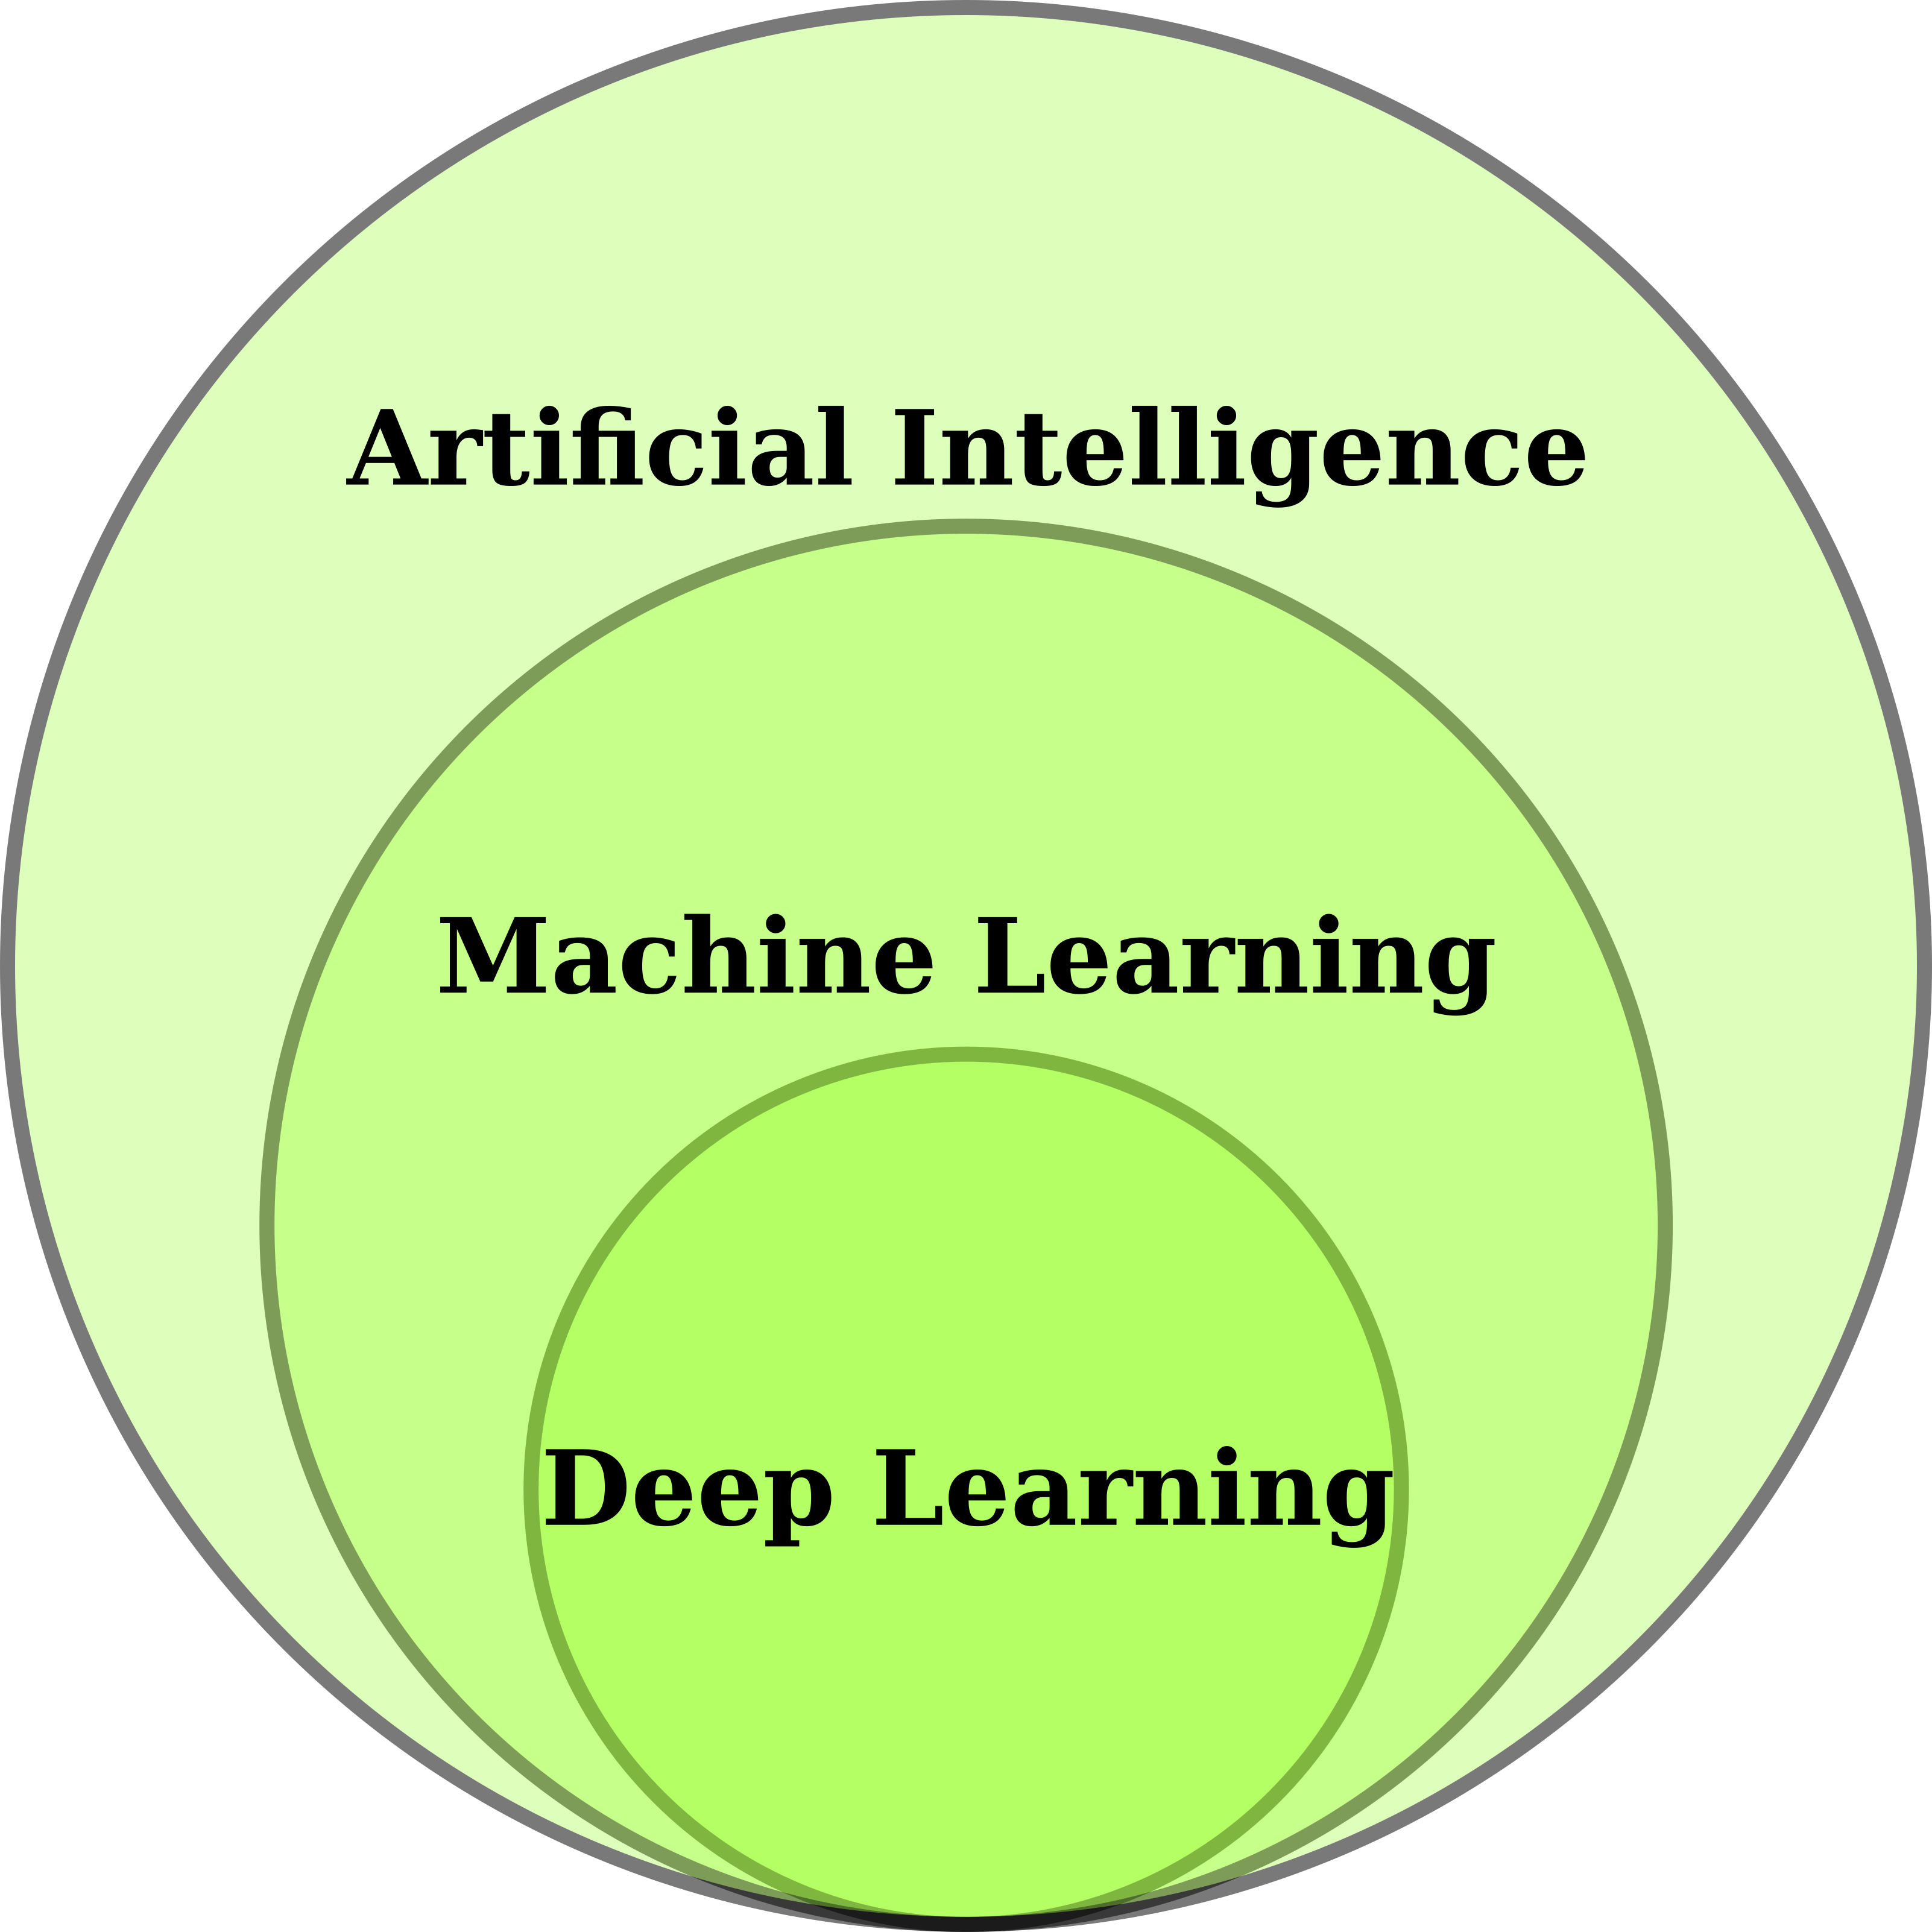
\includegraphics[width=0.6\textwidth]{figures/aimldl.png}
%	\caption{From artificial intelligence to machine learning to deep learning.}
%	\label{fig:aimldl}
%\end{figure}

%\textbf{Training}
%\textbf{Dataset}

% what is machine learning 

% Biological motivation
% Reinforcement, supervised, unsupervised, (semi-supervised)
% What are they capable of? (Some of the greatest works: Machine translation, Image classification, medizine)
% Leserorientierung: In detail which methods exactelly



\section{Artificial Neural networks}
Artificial neural networks are inspired by biological neural systems. Yet strongly simplified, the terminology is oriented on parts of the brain. A first approach for artificial neural networks was introduced by Warren McCulloch and Walter Pitts 1943 in their paper \glqq A logical calculus of the ideas immanent in nervous activity\grqq{} \cite{mcculloch_logical_1943}, where they explain their idea of a computational model which could represent mathematically how animal brains work on the scale of neurons to perform complex tasks. Their neural network is built from binary units with one or multiple binary inputs. It is able to perform simple binary classifications respectively logical computations. However, a more general description of a neuron is a based on continuous calculations, whose mathematical concepts I explain in the following.

\subsection{Mathematical computations in artificial neural networks}
The smallest functional unit of an artificial neural network is the neuron. As mathematical function $f$ it takes a number of weighted scalars and outputs the sum of them. It is a linear function which quantity is represented by a weight-vector $\textbf{w}$ and a bias $b$. The computations of a neuron are 

\begin{align}
    y=f_{\text{neuron}}(\textbf{x})\equiv\textbf{w}^T\textbf{x}+b,
\end{align}
where $\textbf{x}=(x_1,...x_n)^T\in\mathbb{R}^n$ and $b\in\mathbb{R}$.

However, a so-called layer in a feed forward neural network contains a bunch of neurons, the computation for all neurons within the linear part of it thus is written in the form

\begin{align}
    \textbf{y}=f(\textbf{x})\equiv\underline{\underline{\textbf{w}}}^T\textbf{x}+\textbf{b},
\end{align}

with the weight-matrix $\underline{\underline{\textbf{w}}}\in\mathbb{R}^{n\times m}$ and bias-vector $\textbf{b}\in\mathbb{R}^{m}$ with the number of neurons $m$. This computation builds with a so-called activation-function $A$ a single layer in a feed-forward network. Typically, activation-functions are the logistic function 

\begin{align}
    \sigma(y)=\frac{1}{1+\exp^{-y}},
\end{align}

or the rectified linear unit (ReLU-function)
\begin{align}
    \text{ReLU}(y)=\max(0,y),
\end{align}

to mention two of the most frequently used [CITE]. Finally, the computation within a single layer can be written as

\begin{align}
    \textbf{y}=A\circ f(\textbf{x}).
\end{align}

Note that the notation is point-wise, the activation-functions compute every scalar within an input-vector $\textbf{y}$ independently. In figure (\ref{fig:nn_shematic}) the analogy to a biological neural network is visualized, where the weight matrix are represented by connections between neurons and a neuron is represented by the nodes (blue circles). In this case a neural network is shown, where three layer are composed.

\begin{figure}[ht]
    \center
    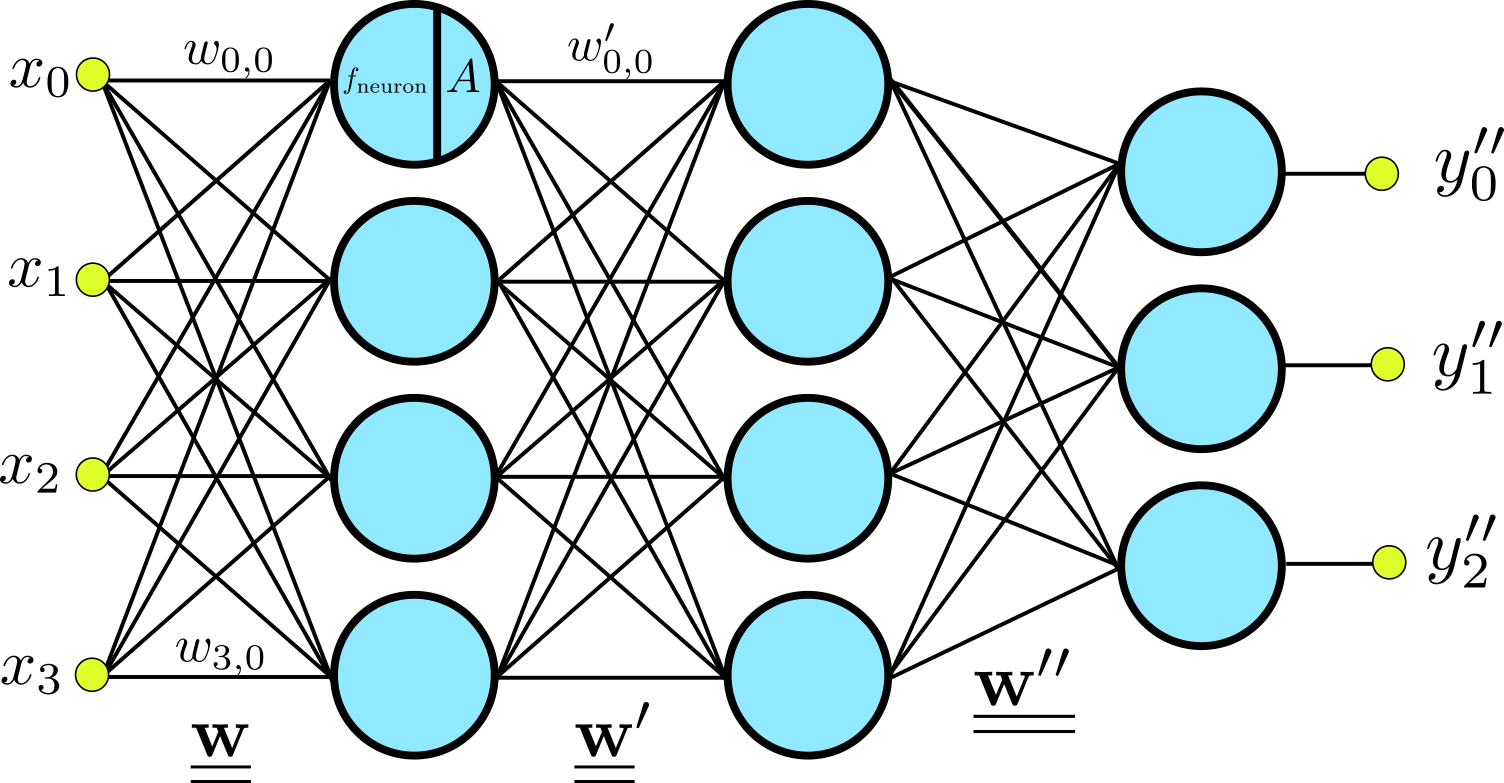
\includegraphics[width=0.8\textwidth]{figures/nn_shematic.png}
	\caption{Schematic view of the computation within a feed forward network, considerably the most simple neural network architecture.}
	\label{fig:nn_shematic}
\end{figure}

The key of a neural network is that the weight matrices and biases are adjusted in a way that the network gives a useful output $\textbf{y}$ regarding a given problem. These parameter will be adjusted in the training process whose fundamentals I introduce in the following section.

\subsection{Training of neural networks}
% What is training briefly
The search for the networks optimal parameter adjustment is called training process. The goal of training a neural network is that the network performs good on yet \textit{unseen} data when the performance is measured by a loss-function, which computes the discrepancy between predictions and the \textit{true values}. Predictions are the output of the neural network, previously noted as $\textbf{y}$ while the \textit{true values} are the aim for what the network should predict, based on a given input. Mostly, the training is a minimization process by applying a distance metric such as mean squared error to quantize the validity of the prediction.

The subject of machine learning can be roughly divided into three areas: Supervised learning, unsupervised learning and reinforcement learning.
Here an input is already assigned to a corresponding output, the relationship which the network is supposed to learn. This type of training process is called supervised learning. Since this work contains of two experiments which focus only on supervised learning, when explaining the training process, I only consider this case.
%(VORHER DEFINIEREN: Data, true values in supervised learning, prediction) 

%Usually, the data set is divided into subsets: The training-data which is used during the training process, and validation data to measure the networks performance, while this data set is not included in the training process.

\subsubsection{Optimization process}
% How does training work
Optimizer are iterative algorithms to find the optimal networks parameter which (mostly\footnote{Dependent on the loss-function, the goal could also be the maximization. Nonetheless every loss-function can be reformulated so that the training process is again a minimization task, without changing the properties of the loss function.}) minimize a loss function $L$. With each iteration, a sub set of the training data called batch is passed to the loss function, whose gradient with respect to the networks parameter $\theta$ is then used to update these parameter. The gradient calculation is performed by the backpropagation algorithm \cite{Rumelhart1986} in the parameter space. There exist a lot different optimizer respectively update-rules, from which I will explain one of the most basic one called \textit{gradient descent}, to have an idea about the general functionality. Every optimizer of this kind is as well based on an update rule including the gradient of a loss function. An update in the \textit{gradient descent} algorithm is computed according to

\begin{align}
    \theta_{\text{new}}=\theta+\eta\cdot\nabla_{\theta}L(f(X|\theta),y),
\end{align}

where $\eta$ is the learning rate, a quantity to adjust how big the network parameters $\theta$ can change within an updated. The right choice of this parameter is critical \cite{wu_demystifying_2019}. There are three types of gradient descent methods which differ in the amount of data to be passed through one iteration. If $X$ contains of one \textit{data-point}, the optimizer performs a parameter update with every single training example. In contrast there is the \textit{batch gradient descent} which calculates the gradient on the whole dataset to perform a parameter update
The third possibility is a compromise of both, where the optimizer only uses a part of the dataset which however contains more than one single example each, to perform one parameter update.

Probably the most famous optimization-algorithm in machine learning is the Adaptive Moment Estimation optimizer (Adam)\cite{adam} which is specifically designed to train neural networks. Firstly introduced in 2014 it showed big performance gains in training speed. In this work I use the same optimizer for every training process.\\

%\textbf{Loss-function}\\
%Previously denoted as $L$, the loss-function is a critical 
%During the training process, one has to face the following problems:\\

\textbf{Overfitting}\\
When training a model on a dataset, we want a loss-function to get smaller during the process according to that dataset, but as well that it can generalize what it learned from the training data on yet unseen data. A problem can appear if the model relies too much on the training data that it even considers secondary patterns like noise, which is a disadvantage for a model which should be able to generalize well. In the example in the left figure of (\ref{fig:underover}) the model predicts very well on the known data, but at the same time is not able to capture the most dominant trend which might be handled better by a regression with squared term. Overfitting can appear if the model is too complex or the model was trained for to many iterations. Staying in the example of figure (\ref{fig:underover}), the model is too complex, while a regression with squared term would perform better. \\

\textbf{Underfitting}\\
The problem of underfitting appears if the model is not capable of processing the complexity of the dataset. Reasons are if the model is not trained enough that did not learn \textit{enough} from the data, or if the model is \textit{too simple}.
An example is visualized in figure (\ref{fig:underover}, right), the model is not able to capture the main trend as well. This is due to the fact that here a linear regression was chosen as model, which is not able to handle a quadratic trend.


\begin{figure}[ht]
    \center
    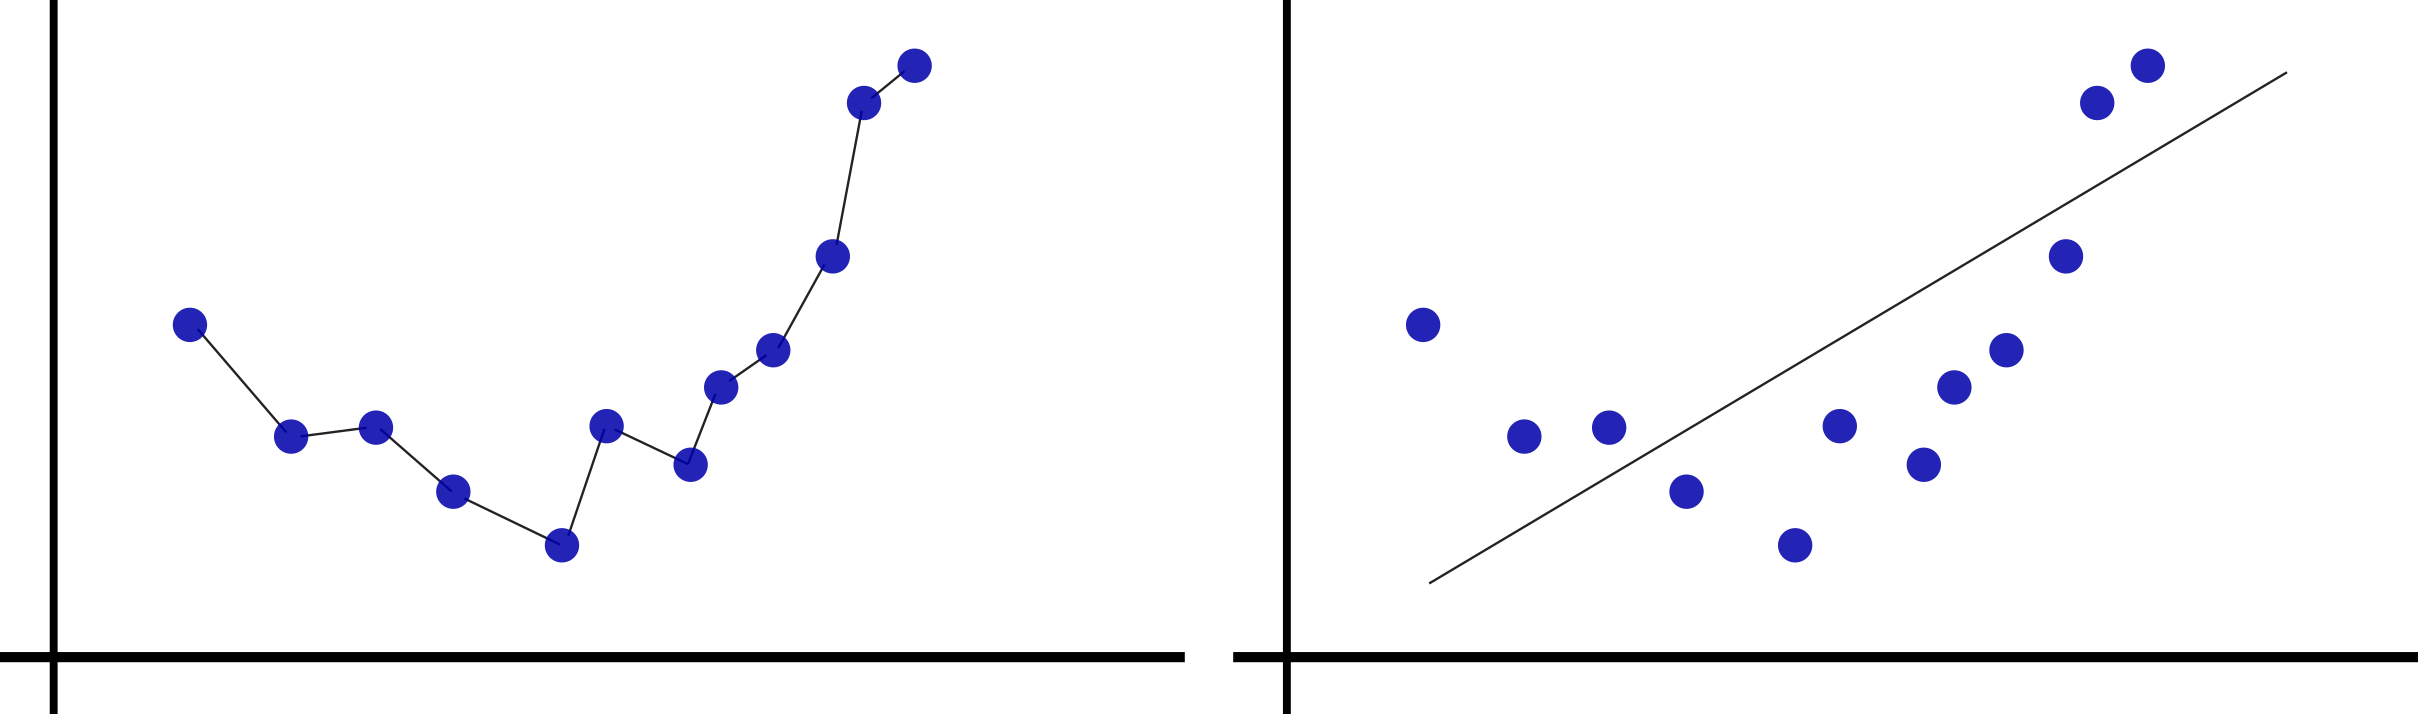
\includegraphics[width=0.99\textwidth]{figures/underoverfitting.png}
	\caption{Easy over and under}
	\label{fig:underover}
\end{figure}

To face these problem, there are a few regularization techniques which I also apply in the neural networks for in this work.

\subsection{Regularization against over- and underfitting}
The following methods to prevent overfitting and underfitting can be divided into two areas: On the one hand, I present methods that are implemented in the form of additional layers in the network (such as dropout and batch normalization), and on the other hand, there are also rules that only take effect during the training. The difference is that one method co-defines the computational graph and may have trainable parameters, while the other methods are applied during the training process.

\subsubsection{Dropout}
By ignoring a set of neurons a neural network can imitate \textit{sub networks} and is therefore able to have a dynamic architecture. The regularization technique called dropout randomly removes neurons during any execution of the network. Firstly introduced by N. Srivastava et al. \cite{srivastava_dropout_2014}, dropout helps to prevent overfitting by not allowing the network to have a rigid architecture which may be too oriented to the training data.

\subsubsection{Batch normalization}
Batch normalization can increase the stability of a neural network by normalizing the input of single layers in the neural network. It can increase the training speed with being able to handle bigger learning rates from the optimizer. Deep neural network are sensitive to the choice of initial weights and the training algorithm respectively the choice of the learning rate. Batch normalization increases the robustness with regard to the choice of these parameters \cite{ioffe_batch_2015}.

\subsubsection{Early stopping}
While the two previous regularization techniques require to be implemented with the neural network, early stopping  is a rule that takes effect during the training process. It interrupts the training process as soon as there is no improvement in the loss for the test set for a longer period, a so-called \textit{plateau}.\\


%The following regularization, which I apply does not face the over- or underfitting problem, but is regarded as 

%\subsubsection{Reduce learning rate on plateau}


\subsection{Convolutional neural networks}\label{cap:convolution}
%Intro, why good, good somewhere else, good in this work.
How neural networks possibly have been inspired by biological brains, convolutional neural networks (CNNs) might have its inspiration from the brain’s visual cortex. They are commonly designed for tasks in computer vision and have been able to achieve state-of-the-art results with models which includes convolutional operations. Examples \textit{EfficientNet} in image classification \cite{tan_efficientnet_2020} or \textit{EfficientPS} in semantic segmentation \cite{mohan_efficientps_2020}. Nonetheless, CNNs are not restricted to computer vision tasks, but also successfully used for example in \textit{ContextNet} for speed recognition \cite{han_contextnet_2020} or in natural language tasks like machine translation as in \textit{ConvS2S} \cite{edunov_classical_2018}. In this work CNNs are used to process electrocardiography signals (See chapter \ref{cap:}). However, I firstly focus on visual tasks to explain the computations behind CNNs since it is most common use case. Later in this work, instead of a 2D image as an input, a 1D ECG-signal is used as well, but the mathematical principles are the same, which can easily be transposed to a lower-dimensional case. 

\subsubsection{Kernel-convolution}
A convolutional neural network is based on the kernel-convolution. It is a discrete operation where a small matrix $W$, called kernel or filter, is passed over an image $I$ and transforms it in dependence of the kernel- and image-values. The operation is computed as 

\begin{align}
    g_{x,y}= W*I_{x,y}=\sum_{dx=-a}^a{\sum_{dy=-b}^b{W_{dx,dy}\cdot I_{x+dx,y+dy}}},
\end{align}

where $a$ and $b$ indicate the size of the kernel $W$. The function is calculated for all $x$ and $y$ on the image on which the filtered image $g$ is based on. 

\subsubsection{Multi-channel convolution} \label{cap:multichannel}
In most images, each pixel is represented by three values which define the color (red, green and blue). The convolutional operation should be able to take these three values (in the following called channels) into account. It is also important that multiple filters can be applied to the image, so that the input image and the output image have multiple channels. A more general description of the kernel-convolution with multi-channel input and output is given by

\begin{align}
    g_{i,x,y}^{\prime}= W_i^{\prime}*I_{x,y}=\sum_{j=1}^N\sum_{dx=-a}^a{\sum_{dy=-b}^b{W_{dx,dy}\cdot I_{j,x+dx,y+dy}^{\prime}}},
    \label{eq:multiinout}
\end{align}

with $N$ as number of channel within the input image (for example $N=3$ in an rgb-image).
Applying (\ref{eq:multiinout}) with every kernel $W_i^{\prime}$ in $\textbf{W}:=(W_1,...,W_M)$ gives a multi-channel output $\textbf{g}_{x,y}^{\prime}:=(g_{1,x,y},...,g_{M,x,y})$. 

\subsubsection{Valid- and same- convolution}
The equations above don't consider yet how the computation looks like at the edges when $x+dx$ or $y+dy$ exceeds the image boundaries. Two common rules are called \textit{valid} and \textit{same}. \textit{Valid}-convolution calculates only values for the respective point $(x,y)$ as far as it lies in the image, while with \textit{same}-convolution, zeros are added at the edge of the input image, so that the filtered image has the same width and height as the input. The parameter to implement these rules is called padding, it specifies the thickness of the additional margins added to the image with zeros.

\subsubsection{Strided convolution and max-pooling}
In previous equations, the kernel is only shifted with a step-size (stride) of one pixel. However, one can increase the step-size if $\textbf{g}$ should have smaller spatial dimensions. Furthermore, as consequence of a bigger stride, each pixel in $\textbf{g}$ is dependent of a bigger sub-field, the so-called \textit{receptive field} on the input image. The size of this field is important for processing spatial relationships within the image [CITE].

While \textit{stride} is a hyperparameter of the kernel-convolution operation, \textit{max-pooling} is a technique that functions as an independent layer in a neural network. It divides the input (here a 2D-image) into subsets like 2$\times$2-fields of spatial neighbouring pixels and outputs only the maximal image value of each. This technique reduces the spatial dimension of the input as well, and increases the receptive field. \\

In this work, convolution-layers are implemented within neural networks of both experiments. The first experiment applies a 1D-convolution to process through electrocardiography-signals, while in the second experiment, 2D-convolutions are used to encode spatial correlations and decode a low dimensional representation of images.

The chapter showed how convolutional neural networks process through spatial\footnote{The terminology \textit{spatial} does not necessarily refer to data points that are spatially related. It is to be understood more generally in the sense that data points, such as the pixels of an image, in the form in which they are stored (as a 2D array in this example) also contain information through their position and their neighbors.} correlations. In the next chapter I introduce recurrent neural networks, which are designed to process temporal dynamics in sequences.

\section{Recurrent neural networks}
%Intro (what problems for example)
The prominent domain for recurrent neural networks are sequence-to-sequence problems.
It is about training neural networks to convert a sequence to another sequence. A famous task in this domain is machine translation where a sequence of words in one language is transformed to another sequence of words of a different language. Other important tasks are for example speech-recognition where an encoded voice recording has to be converted into a sequence of words, or next-frame-prediction, a task to predict the future frames of a video. In each example, recurrent networks were considered as state-of-the-art, at least for a while. [CITE]

% public datasets
%A large number of famous problems are connected to public data sets, where models can be tested and compared with each other. Furthermore, several validation metrices

% Problems
A characteristic that is generally seen with sequence-to-sequence (seq2seq) problems is that the sequences are of variable length. For example, a translation-model has to be able to take a sequence with varying length of words to output a translation as a sequence with a varying length as well. Furthermore a strong translation model should be able to translate single words as well as a long sequences of hundreds of words. In this work, in the second numerical experiment (VERWEIS HIER) also faces the characteristic of variable input-output length, where a recurrent neural network is used as well.
Therefore, a key feature of machine learning models, designed for seq2seq problems, are their ability to handle sequences of different lengths. In the following, I introduce the smallest functional unit of a recurrent neural network, the \textit{recurrent unit}.

% Models
\subsection{The recurrent unit}
% Introduction
The recurrent unit is a form of neural network which is, in combination of an iterative approach, able to process through an input sequence with varying length. Recurrent neural networks (RNNs) which are built of one or multiple recurrent units (for example stacked into deep RNNs) can be regarded as a generalization of a neural network. With every iteration a \textit{hidden state}, which has a fixed dimensionality, is evolving to be dependent on every time step before. The \textit{hidden state} can be calculated, regardless of the length of the input sequence, and provides a representation of the sequence. \\

% Exact definition
The following equations are the computations within a very basic recurrent unit which builds the so called Elman network \cite{elman_finding_1990}. Given a sequence of inputs $(x_1,x_2,...,x_T)$, the hidden-state $h_t$ evolves as

\begin{align}
    h_{t}&=f_h(\textbf{W}_{x}\cdot x_t + \textbf{W}_h\cdot h_{t-1} + b_h),\notag\\
    y_t&=f_y(\textbf{W}_y\cdot h_t + b_y).\notag\\
    \label{eq:vanillarnn}
\end{align}

Furthermore it gives an output sequence $(y_0,y_1,...,.y_T)$ of the same length as the input sequence, which is taken into account in deep recurrent neural networks by stacking multiple RNNs. The functions $f_h$ and $f_y$ are activation functions like $\tanh$ or the sigmoid-function. \\

\subsubsection{Extensions}

\textbf{Bidirectional RNN}\\
Bidirectional RNNs combine the input sequence and the inversion through time of the same sequence. It can be regarded as an implementation of two independent RNNs which compute through the forward and backward direction of the input, whose output is stacked together. With this form of RNNs the output layer can combine information from the past and future and was firstly introduced by M. Schuster et al. in 1997 \cite{schuster_bidirectional_1997}.\\[1em]
\textbf{Stacked RNN}\\
RNNs can be stacked by taking the output sequence ($y_1$, ..., $y_T$) or the sequence of hidden states ($h_1$, ..., $h_T$) as input for a new RNN. Although it is not theoretically clear why stacked RNNs perform in certain tasks better than single-layer RNNs, in practise it provides a higher learning capacity \cite[p.51]{goldberg_primer_2015}.

\subsubsection{Training of recurrent neural networks}
The computation of the gradient of recurrent neural networks it is not possible by the normal backpropagation algorithm. However, there is a generalization of it called \textit{backpropagation through time} or \textit{BPTT}. The key behind this algorithm is to unfold the network through time into a feed forward network with multiple layers. Therefore the depth depends linear on the length of the input sequence. 

During training the gradient tends to vanish or explode, as firstly discovered by Hochreiter in 1991. He described it as follows:\\ \textit{With conventional \glqq Back-Propagation Through Time\grqq{} [...], error signals \glqq flowing backwards in time\grqq{} tend to either blow up (1) or vanish (2): the temporal evolution of the backpropagated error exponentially depends on the size of the weights. Case (1) may lead to oscillating weights, while in case(2) learning to bridge long time lags takes a prohibitive amount of time, or does not work at all.} \cite{kolen_gradient_2009}.\\
Within the learning algorithm gradient descent, which includes backpropagation, these difficulties are theoretically validated with any loss function \cite{bengio_learning_1994}. Various methods have been proposed to deal with the problem of vanishing and exploding gradient, whereby the most successful is the Long-short-term-memory (LSTM). Hochreiter and Schmidhuber introduced a special kind of RNN in 1997 which is able to prevent the problem of vanishing gradient.

\subsection{Long-short-term-memory}
%\textcolor{red}{LSTM networks were specially designed to learn long-term dependencies and avoid the vanishing gradient problem. The central idea is to have a recurrent edge within each cell that has a weight w = 1. This eliminates the problem of the vanishing gradient problem, as recurrent multiplication by 1 does neither diverge norconverge to zero. To still enable a LSTM to learn a process called constant error carousel controlsthe cell state from one sequential step to the next without any weights being multiplied directly. In-formation flows on two levels from one step to the next while the update of the weights is con-trolled by so-called gates. Gates use different activation functions to forward or stop the informationflow.}

LSTMs work on the same principle as RNNs by evolving a hidden state through an input sequence, but they use a different function to compute the hidden state which furthermore includes an additional state, the \textit{cell state}. With the computations in a LSTM unit it is provided that the gradient of the cell state can be unchanged through time. It is possible to process long term dependencies in a sequence more efficiently. Furthermore, a LSTM overcomes the problem of a vanishing gradient.

The calculations within a LSTM unit it given by

\begin{align}
    g_t&=\tanh\left(\textbf{W}_{cx}\cdot x_t + \textbf{W}_{ch}\cdot h_{t-1} + b_g\right), \notag\\
    i_t&=\sigma\left(\textbf{W}_{ix}\cdot x_t + \textbf{W}_{ih}\cdot h_{t-1} + b_i\right), \notag\\
    f_t&=\sigma\left(\textbf{W}_{fx}\cdot x_t + \textbf{W}_{fh}\cdot h_{t-1} + b_f\right), \notag\\
    o_t&=\sigma\left(\textbf{W}_{ox}\cdot x_t + \textbf{W}_{oh}\cdot h_{t-1} + b_o\right), \notag\\
    C_t&=f_t\circ C_{t-1}+i_t\circ g_t, \notag\\
    h_t&=o_t\circ\tanh(C_t),\notag\\
    \label{eq:lstm}
\end{align}

where $\circ$ denotes the Hadamard product, also known as pointwise-multiplication.

% introduction

% problems


% model to furthermore face these problems
\subsection{Variations and extensions}\label{cap:variationsextensions}

\subsubsection{Convolutional LSTM}\label{cap:CLSTM}
At least since the performance of convolutional neural networks (CNNs) in the ImageNet competition, it is empirically proven that CNNs are more effective and efficient in certain computer vision tasks like image classification than fully connected neural networks.
In the field of sequential learning, computer vision tasks are also formulated, such as video-classification or video-frame interpolation. However, the LSTM as implemented in (\ref{eq:lstm}) can be regarded as recurrent extension of a fully connected neural network, which is not as efficient in processing spatial correlations as a CNN. 

A LSTM with convolutional structure addresses this problem. It is better performing in certain tasks which include spatio-temporal data, as proven for example from Wu et al. for future video synthesis \cite{wu_future_2020}. Therefore, this concept is used in the second numerical experiment of this work, which also deals with the processing of spatio-temporal data.

The equations which build a convolutional LSTM are shown below:

\begin{align}
    g_t&=\tanh\left(\textbf{W}'_{cx}*x_t + \textbf{W}'_{ch}* h_{t-1} + b_g\right), \notag\\
    f_t&=\sigma\left(\textbf{W}'_{fx}* x_t + \textbf{W}'_{fh}* h_{t-1} + b_f\right), \notag\\
    i_t&=\sigma\left(\textbf{W}'_{ix}* x_t + \textbf{W}'_{ih}* h_{t-1} + b_i\right), \notag\\
    o_t&=\sigma\left(\textbf{W}'_{ox}*x_t + \textbf{W}'_{oh}* h_{t-1} + b_o\right), \notag\\
    C_t&=f_t\circ C_{t-1}+i_t\circ g_t, \notag\\
    h_t&=o_t\circ\tanh(C_t).\notag\\
\end{align}

As introduced in chapter \ref{cap:convolution}, the symbol * denotes a discrete convolution while the operator $\textbf{W}'$ are convolutional kernel. The linear operators are replaced by convolutions, that the input of a convolutional LSTM can handle a sequence of spatial data without flattening them to a vector.

\subsubsection{Spatiotemporal LSTM} \label{cap:STLSTM}
%The performance of a LSTM network depends on how good it is capable of memorizing relevant structures. 
As introduced before, a convolutional LSTM is taken into account advantages of convolutions to compute spatial correlation more efficiently. However, in a stacked convolutional LSTM, spatial correlations and temporal dynamics are not equally processed.
But these two aspects might be equally important and have to be considered equally significant in a machine learning model for spatio-temporal data. To address this problem, Y. Wang et al. introduce in their paper "PredRNN: Recurrent Neural Networks for Predictive
Learning using Spatiotemporal LSTMs" \cite{prednet} a variation of the LSTM-cell and its integration into a stacked network. They formulate the problem as follows:\\
\textit{[...] spatial representations are encoded layer-by-layer, with hidden states being delivered from bottom to top. However, the memory cells that belong to these [...] layers are mutually independent and updated merely in time domain. Under these circumstances, the bottom layer would totally ignore what had been memorized by the top layer at the previous time step.}\\

The equations for the spatio-temporal LSTM (ST-LSTM) are given by

\begin{align}\label{eq:stlstm}
    g_t&=\tanh\left(\textbf{W}'_{cx}*x_t + \textbf{W}'_{ch}* h_{t-1} + b_g\right),\notag\\
    i_t&=\sigma\left(\textbf{W}'_{ix}* x_t + \textbf{W}'_{ih}* h_{t-1} + b_i\right),\notag\\
    f_t&=\sigma\left(\textbf{W}'_{fx}* x_t + \textbf{W}'_{fh}* h_{t-1} + b_f\right),\notag \\
    C_t&=f_t\circ C_{t-1}+i_t\circ g_t,\notag\\
    g'_t&=\tanh\left(\textbf{W}''_{cx}*x_t + \textbf{W}'_{cm}* M^{l-1}_{t} + b'_g\right),\notag\\
    i'_t&=\sigma\left(\textbf{W}''_{ix}* x_t + \textbf{W}'_{im}* M^{l-1}_{t} + b'_i\right),\notag\\
    f'_t&=\sigma\left(\textbf{W}''_{fx}* x_t + \textbf{W}'_{fm}* M^{l-1}_{t} + b'_f\right),\notag\\
    M^{l}_t&=f'_t\circ M^{l-1}_t+i'_t\circ g'_t\notag\\
    o_t&=\sigma\left(\textbf{W}'_{ox}*x_t + \textbf{W}'_{oh}*h_{t-1} + \textbf{W}_{om}*M_t^l + b_o\right),\notag\\
    h_t&=o_t\circ\tanh(\textbf{W}_{1\times 1}*\left[C_t^l,M_t^l\right]).\notag\\
\end{align}

The idea behind this LSTM-adaptation is visualized in figure (\ref{fig:seq2seq}). With each layer, the spatial representation develops within an additional cell-state $M$ with each layer and is then passed to the bottom layer of the next time-step. 

\begin{figure}[ht]
    \center
    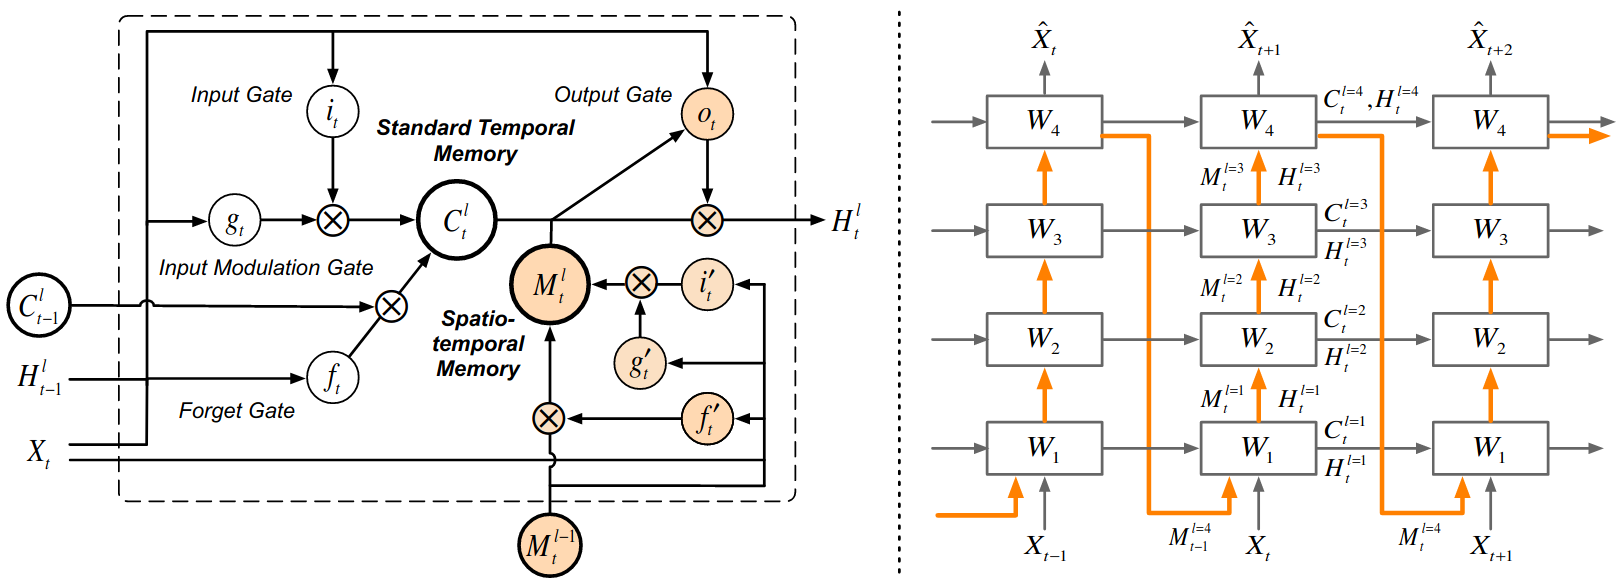
\includegraphics[width=0.99\textwidth]{figures/stlstm.png}
	\caption{Spatiotemporal LSTM, (left) the computations inside the ST-LSTM-cell, (right) the unfolded cell through time. The orange arrow marks the spatial flow through layer and time-step.}
	\label{fig:seq2seq}
\end{figure}

LSTMs are the favored implementation of recurrent networks, it is a standard to overcome general problems like vanishing gradient and learning long-term dependencies. Additionally, convolutional LSTMs or spatio-temporal LSTMs are designed to specifically face problems which occur in deep LSTMs where spatial correlation and temporal dynamics are not equally processed.

Although recurrent cells have been mentioned so far, it is not yet clear how exactly this iterative process can be used to process a sequence2sequence problem.
\section{Seq2Seq-models}\label{cap:seq2seq}
%introduction, and problems to face
A seq2seq LSTM-neural network is a type of encoder-decoder model, consisting of two LSTMs, one for encoding the sequence to a \textit{thought vector} of fixed dimension, and the other for generating an output sequence with varying length from the thought vector. Furthermore, each time-step of the input might be processed by an encoder independently, as well as the output sequence steps by a decoder as visualized in figure (\ref{fig:seq2seq}). %While there are several slight variations, which data is passed to the decoder-LSTM, in this work for the experiment in chapter 4, the same hidden-state $h_T$ (part of the thought-vector) is the input for every time-step.
% encoder-decoder models

\begin{figure}[ht]
    \center
    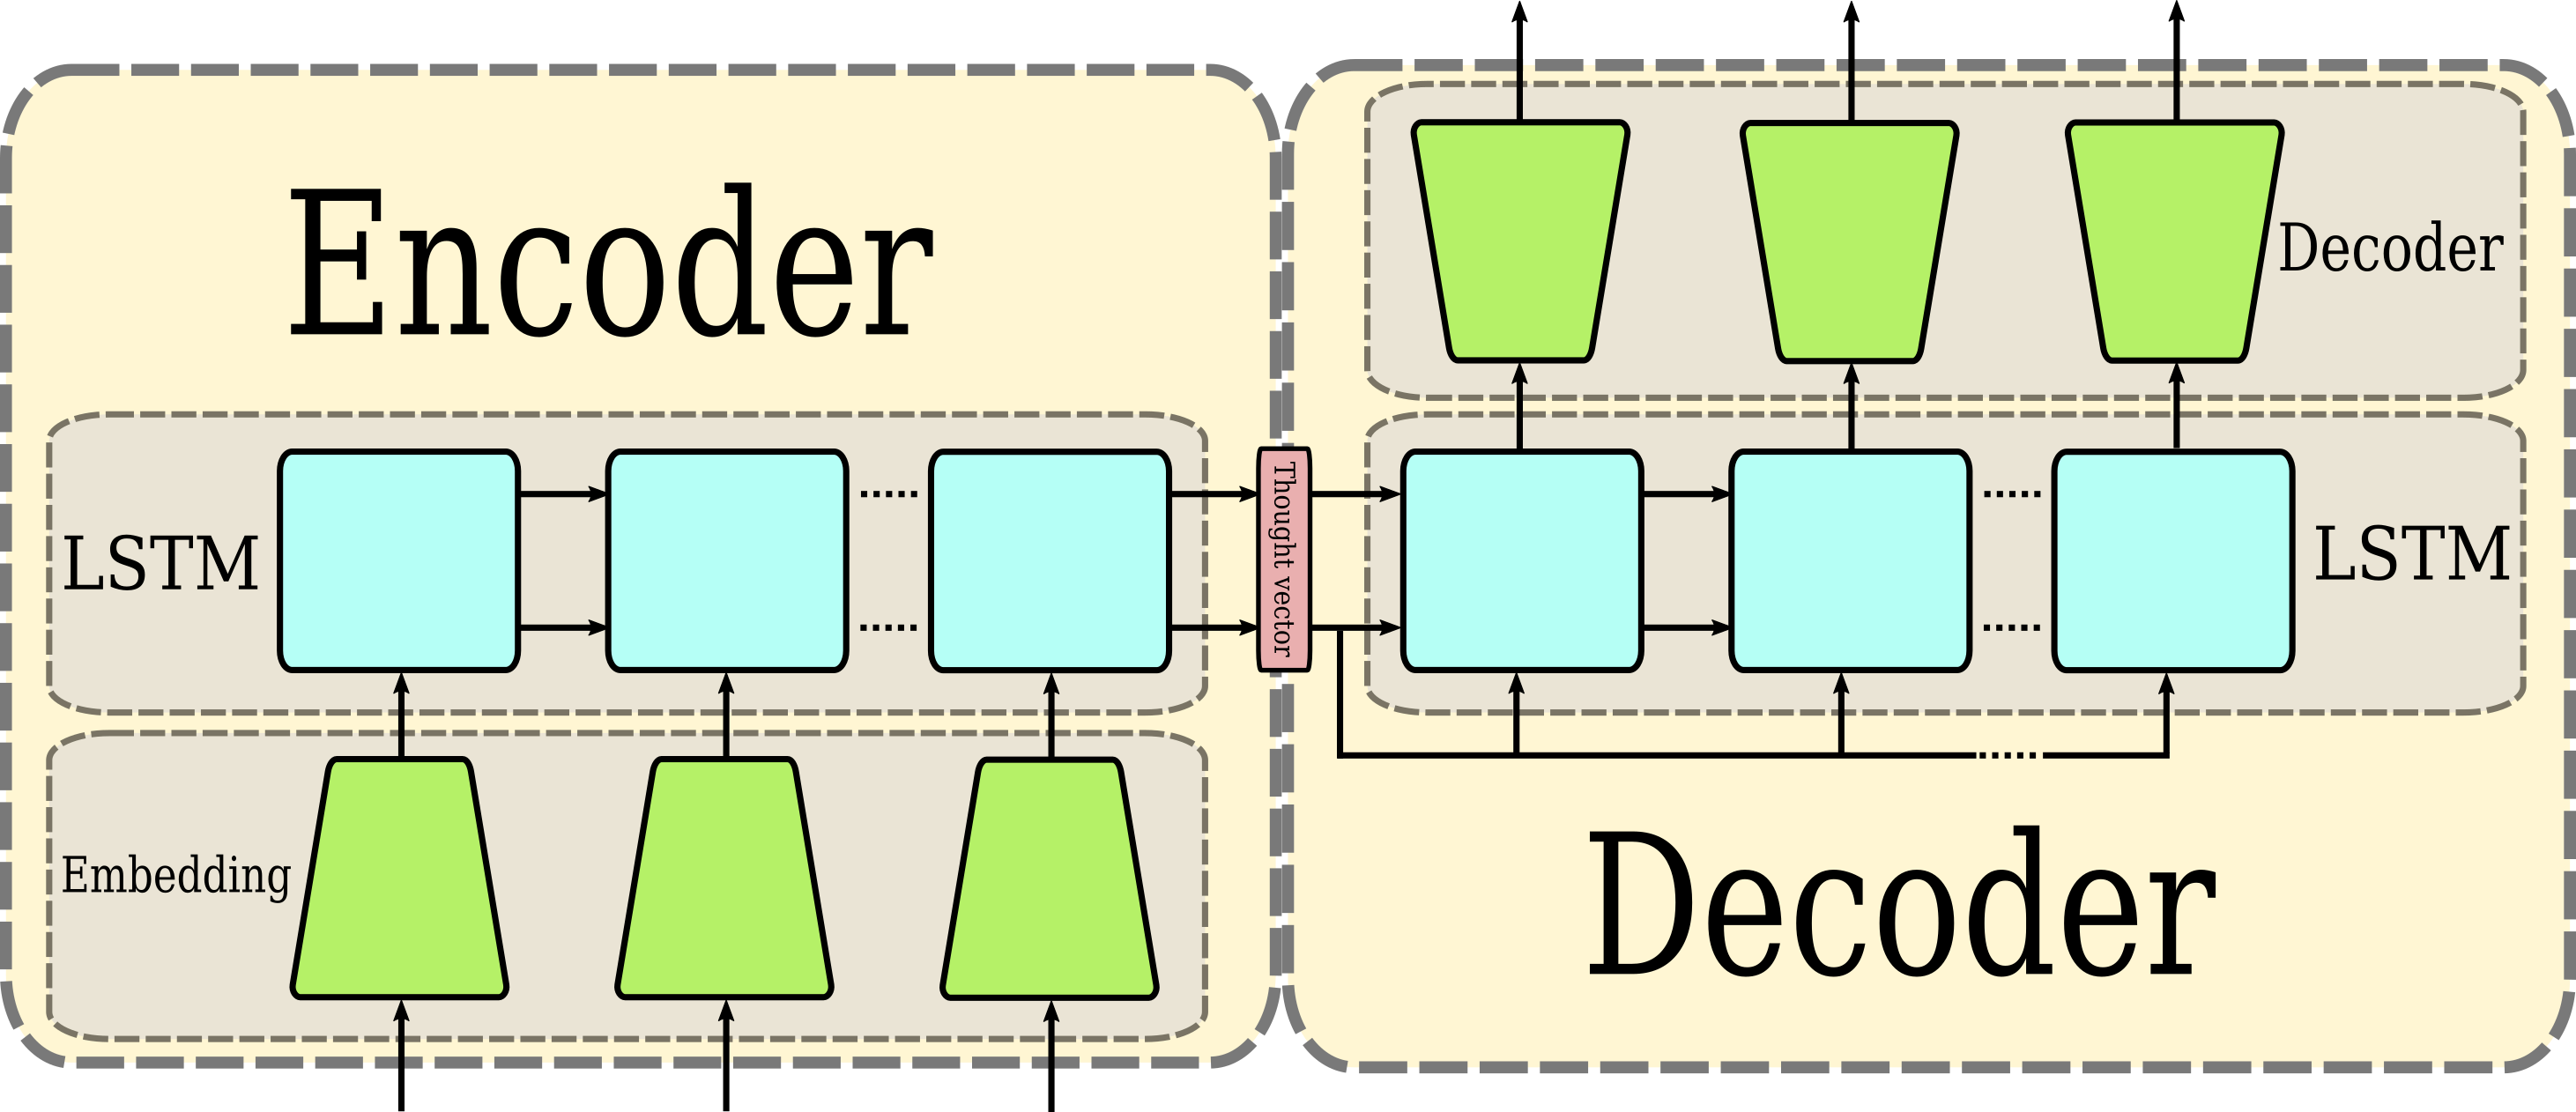
\includegraphics[width=0.99\textwidth]{figures/seq2seq.png}
	\caption{Schematic sequence to sequence model with an encoder-decoder structure.}
	\label{fig:seq2seq}
\end{figure}

%\subsection{Regularization techniques}

\section{Tools}
This chapter gives a short overview of the used software and libraries.

\subsection{Python}
\textcolor{red}{Python is a high level, general purpose programming language distributed by the Python Software Foundation (“Python – SF”). Python was first released in 1991. The current Python 3 version,which is used in this thesis, was released in 2008. It runs through an interpreter, thus python code can be run without the need to compile it. This allows for fast development and testing of code. Due to this and the huge amount of external libraries python is a widely used language in many scientific projects. It is also one of the most used language to develop NNs because it offers many powerful DL libraries, e.g. TensorFlow, Pytorch, Theano, Caffe etc. Furthermore, Python offers an almost limitless amount of other libraries useful for data preprocessing. The following three libraries wereused for this purpose:1.Numpy Numpy is a module that allows for scientific computing in Python. Its most used feature, in the context of this thesis, is the creation, editing and calculation of N-dimensional array objects (“NumPy”).}

\subsection{Keras}
\subsection{PyTorch} \label{cap:pytorch}
PyTorch \cite{pytorch}is an open-source machine learning framework, based on Torch \cite{torch}, which is the chosen API behind the majority of state-of-the-art models. By current status\footnote{According to the status in September 2020}, pytorch is the most popular framework of its kind. Together with keras (the second most used API) around 66\% of all papers based on machine learning research have used at least one of these APIs.
They support the most commonly used methods such as convolutions, LSTMs in a high abstraction.

\subsubsection{Automatic differentiation in PyTorch}


    \chapter{The inverse problem of electrocardiography}
%In this chapter I will firstly give a short introduction of the biological background, which makes it possible to measure a potential difference between two electrodes on the torso surface. As the heart with its electro-chemical activity dominates these measurements, I will give a short overview over the anatomy and give an insight into the hearts smallest functional unit, the heart muscle cells. Furthermore a short introduction into the electrocardiography is given, TODO

% Shortly what is inverse problem, and explanation of terminology.
In broad terms, the inverse problem of electrocardiography (iECG) is about gaining knowledge about the activity of the heart, based on measurements from electrodes on the torso surface \cite[p.300]{iECG} Based on this definition, the experiment described below can also be understood as the processing of the inverse problem of ECG. The aim of this study is to find out to what extent it is possible to differ between several pattern in the heart's activity through ECG measurements. 

One of the most important use case of ECG measurements is the classification of the corresponding activity of the heart. [...]
A much more difficult task is the complete reconstruction of the cardiac activity or the surface activity using the ECG signals. Mathematically, this can be described as ill-posed, which in our case means that a possible solution is not unique\footnote{According to the definition of Jacques Hadamard [CITE] a problem is well-posed if (1.) a solution exist, (2.) the solution is unique, and (3.) the solution depends continuously on the data. A problem is ill-posed if it fails to satisfy one or more of these conditions}.
[...]
Therefore, it can be said that the inverse problem of electrocardiography is an important topic in medicine which potential is not yet exhausted.
%In this experiment 
%The aim of this study is to find out to what extent it is possible to quantitatively characterize a structure, by locating the source of concentric waves originating on the heart surface, based on ECG measurements. The data are based on the simulation of the electrical activity of a porcine heart and corresponding ecg signals.

%The terminology inverse indicates that there is a 'forward' problem of ECG. 

%While within the inverse problem, the potential differences at the torso are tried to trace back (inverse) to its source, the forward direction is regarded as the computation of the electric potential 

%as the tracing back of the activity to gain information of the heart's behavior, without directly measuring on its surface.

%The term “forward problem of electrocardiography” is used to denote the computation of the electric potential field generated by cardiac excitation within and on the torso surface.

%The terminology inverse indicates that there is a 'forward' problem of ECG.

%The mathematical description of the propagation of the electrical signals which are coming from the heart and are propagating through the body onto the body surface, is described as 'forward'. The forward propagation is measurable through potential differences between two electrodes on the torso.

%The terminology inverse indicates that there is a 'forward' problem of ECG. The formulation is based on the fact that the electro-chemical activity of the heart is measurably 

%Since the electro-chemical activity of the heart is measurable 

%The terminology inverse indicates that the measurements have 
%The terminology inverse indicates that there is a forward direction. 
\section{Problem formulation}
% Was in etwa
As already briefly explained, this experiment is about the differentiation of activities of the heart, which are characterized by different spatio-temporal excitation patterns. A representation of this activity is provided by the measurements of electrodes at a certain distance from the heart.

% Wie wird es verwirklicht
In this experiment, the data of the electrical activity of the heart as well as the corresponding ECG signals through the electrodes are simulated (see section \ref{cap:simulation} for more details about the simulation). It is a simulation of a pig's heart whose geometric shape comes from a CT-scan. The electrodes are set up at a certain distance within two grids as visualized in figure (\ref{fig:heart_overview}). Four electrodes are marked in the graphic from which a virtual reference electrode is calculated whose geometric center lies approximately in the middle of the heart. All electrodes of the two grids have the same reference electrode.

% Wie wird das Problem verwirklicht
Different excitation patterns are generated by stimulating a previously defined point on the heart surface at a constant frequency, where the position varies in every simulation. This pacing induces a concentric waves which spreads over the entire heart. The aim of this experiment is to predict the position where the pacing events are happening, based on the ECG-signals.

% Daten und was damit angestellt wird.
A simulation generates ECG data in the form $X_{\text{ECG}}\in\mathrm{R}^{T\times N}$ where $T$ is the number of discrete time steps and $N=70$ the number of leads (respectively electrodes, each lead is built with the same virtual electrode). The exact spatio-temporal activity of the heart is not recorded as it is not relevant for the prediction. Only the position of the pacing is stored as a 3-dimensional vector. The selection of the relevant parameters $T$, $N$ and the conversion of the discrete quantities (time and space) into characteristic quantities are described in chapter \ref{cap:simulation} (simulation) respectively \ref{cap:processing} (data processing). 

% Was macht man mit den Daten
%To pose the problem to an algorithm, the 


\begin{figure}[ht]
    \center
    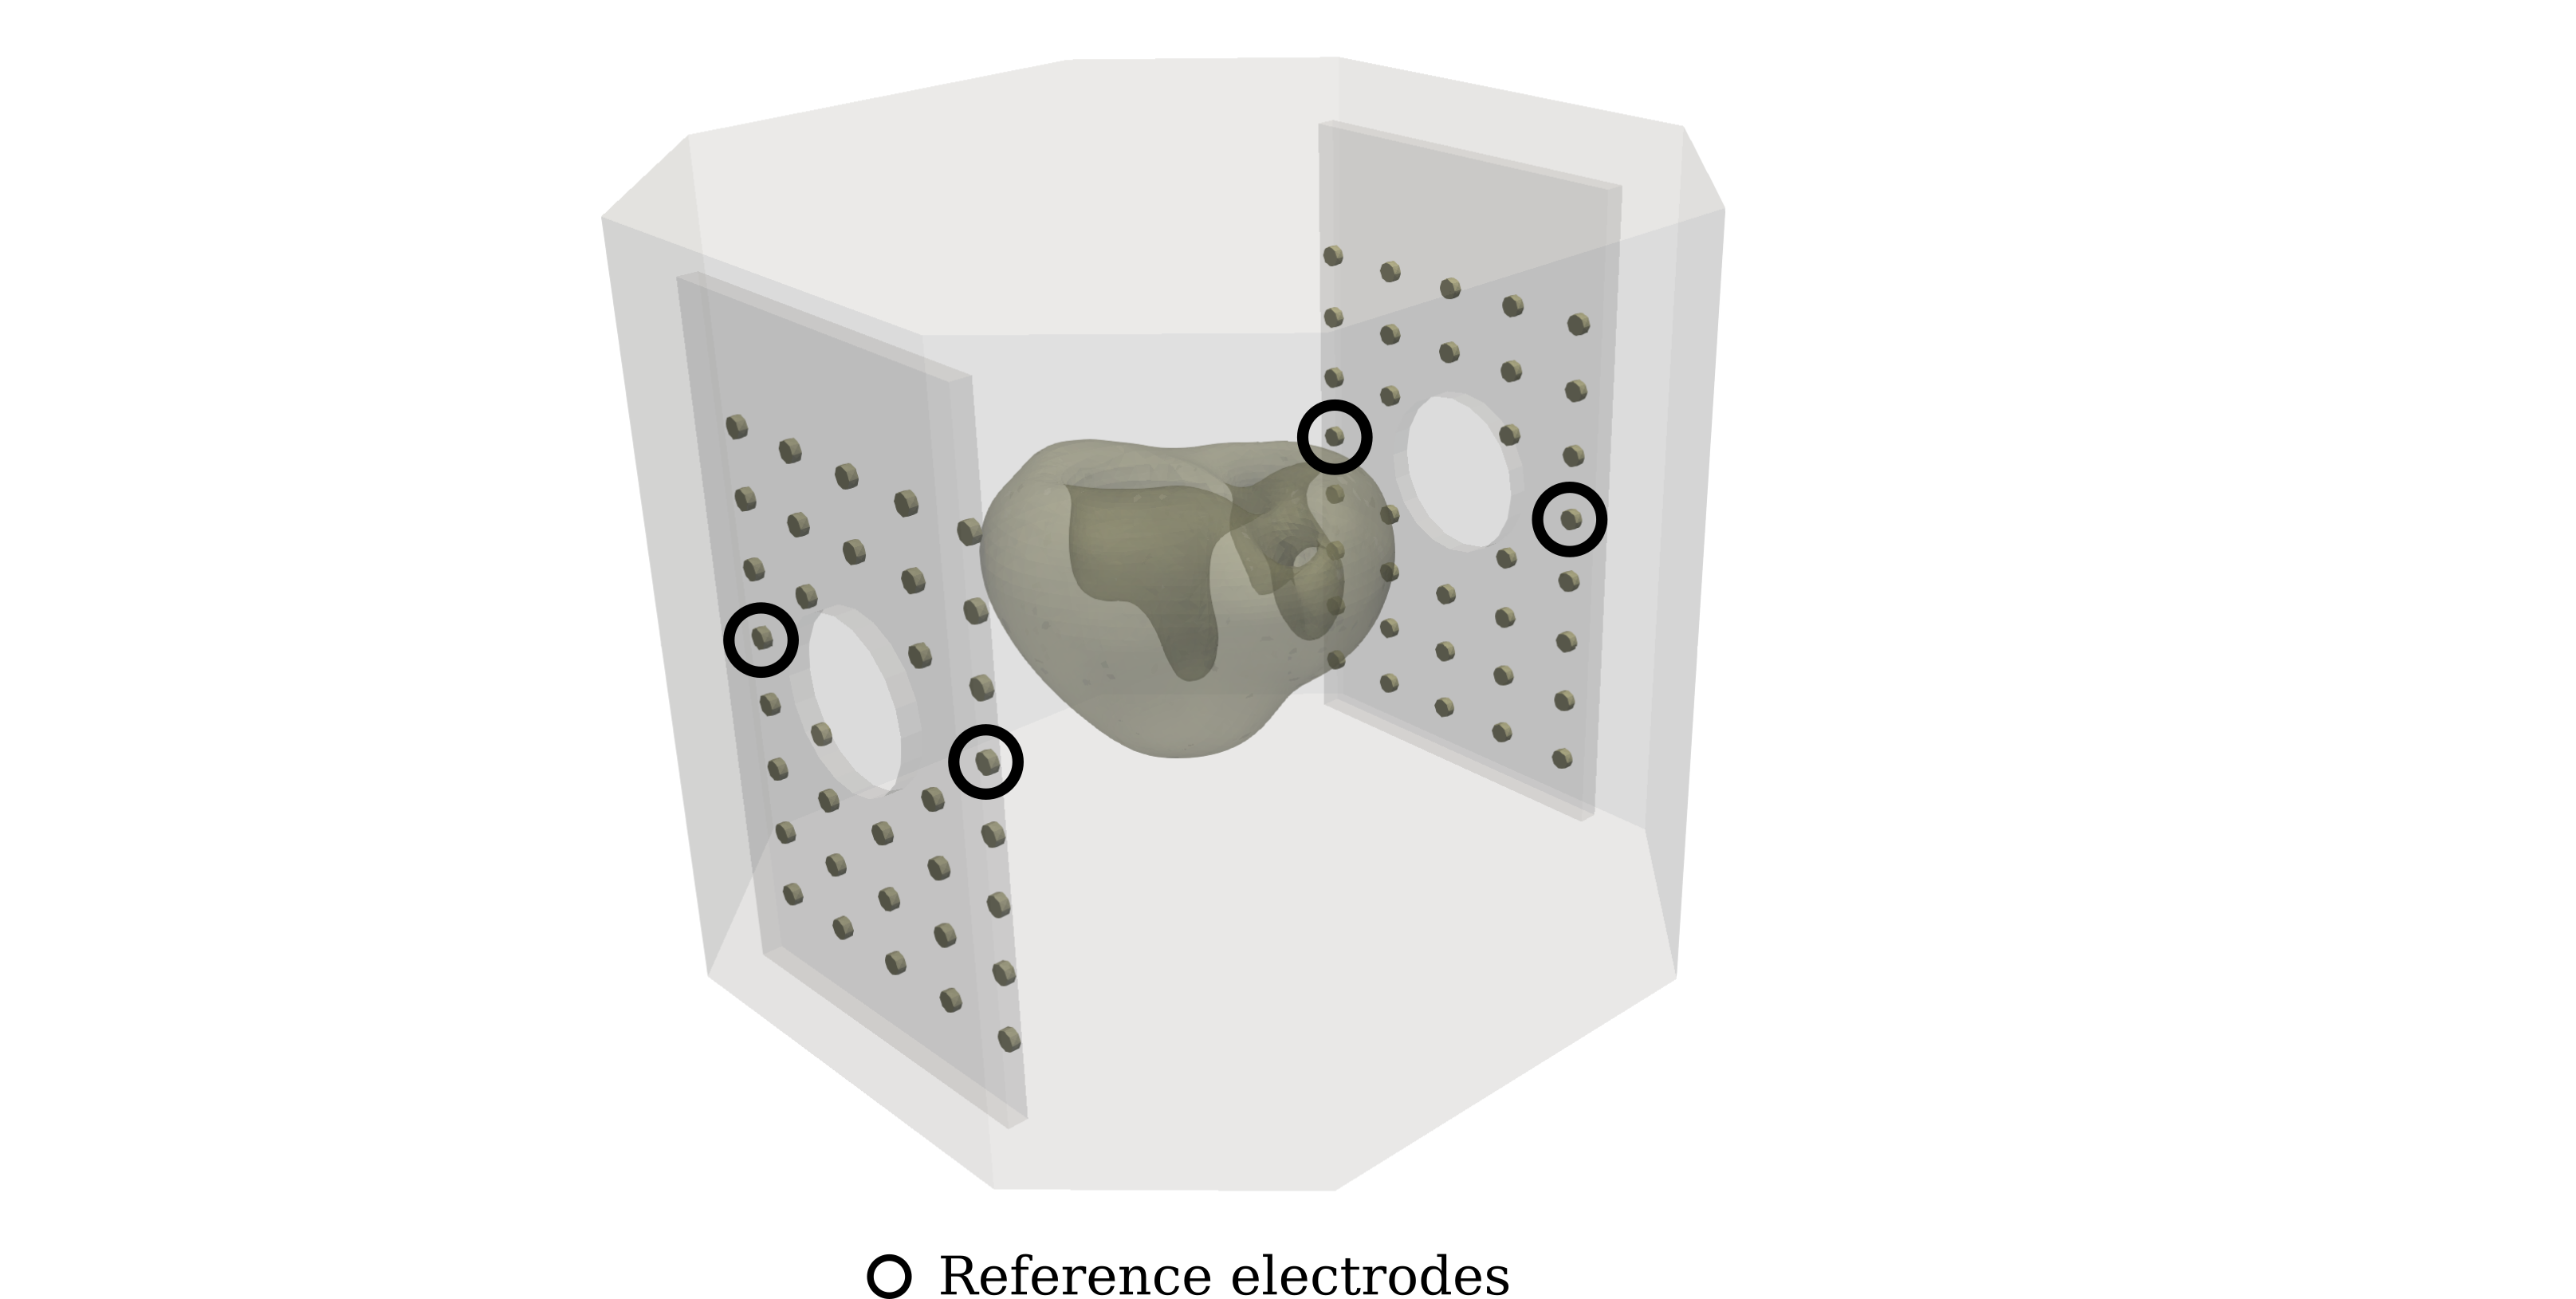
\includegraphics[width=1.3\textwidth]{figures/heart_overview_inkscape.png}
	\caption{Easy}
	\label{fig:heart_overview}
\end{figure}


%As already briefly explained, this experiment is about the differentiation of dynamics in the form of the electrical activity of the heart. The starting point for generating different types of dynamics is an unexcited heart. During the simulation, a point on the heart surface is stimulated with a constant frequency, from which a concentric wave spreads over the entire heart. What an excitation means in this context is described in chapter xx, as well as the biological mechanisms of electrical stimuli transmission so that a concentric wave can arise is described in chapter yy. 
%The location of the stimulation is varied in a number of simulations. the corresponding ECG signals are the input of a neural network, which is supposed to predict the exact location of the stimulation.


%It provides a multi channel-ECG 
%The problem 
%he aim of this study is to find out to what extent it is possible locating the source of concentric waves originating on the heart surface. 
%The data are based on the simulation of the electrical activity of a porcine heart and corresponding ecg signals.
% What is the problem in this work

% why is it important?

\subsection{Related work}
% A few paper
% Problems
\textcolor{red}{A few paper, problems}

% Leserorientierung 
Since the experiment involves the simulation of electrical propagation in cardial tissue, the biological background is first explained in the following chapter. 
%In the following chapter I will give a brief overview of the biological background behind the simulations. This includes the functionality of the heart and the technique of measuring its activity indirectly, the electrocardiography (ECG).


%\textcolor{red}{This numerical experiment tries to find the source of a induced concentric wave, based on multiple ECG signals. The input is multi-channel time-series with dimension $R^{N\times T}$ The output is a 3d-coordinate $\in R^{3}$, therefore the problem is a regression.}

\section{Biological background}
This chapter gives an overview of the anatomy of the heart and its smallest functional units, the cardiac muscle cells. The coordinated contraction of these cells leads to a pumping action of the heart. Within a repetitive pumping process, blood is enriched with oxygen within a heart chamber and passed on to the body. In the following I briefly explain how the anatomy of the heart makes this process possible, as well as discuss the electro-chemical properties of cardiac muscle cells, to understand its coordinated contraction through signal propagation which lead to the pumping effect.

%The mathematical description of the propagation of the electrical signals which are coming from the heart and are propagating through the body onto the body surface, is described as 'forward'. The forward propagation is measurable through potential differences between two electrodes on the torso. In following, I will explain the electro-chemical characteristics of the heart and its spatio-temporal behavior. In the terminology in which the mapping from the activity of the heart to a distant medium (like the torso) is described as forward problem, the inverse problem is defined as the tracing back of the activity to gain information of the heart's behavior, without directly measuring on its surface.

%What is the basis of the heart
% (Leserorientierung: Physiology, heart muscle cells)
\subsubsection{Anatomy of the heart}
This section is based on chapter 1 of the book \textit{Herz-Kreislauf} by J. Steffel and  T. Lüscher \cite{kreislauf}.
The heart consists of four chambers, the left and the right atrium and the left and the right ventricle, as visualized in figure (\ref{fig:heart_anatomy}). The right atrium with the right ventricle builds the right half of the heart, which pumps the blood to the lungs for a gas exchange. From there the blood flows towards the left half of the heart (which consists of the left atrium and the left ventricle). The left half of the heart pumps the oxygen-rich blood towards the individual organs. The heart beats between 50 and 80 times a minute in normal condition. The pumping is caused by an electrical impulse, initiated by the sinus node. The pulse (action potential) is a rapid potential change of the membrane potential induced by moving ions through the cell membrane. The pulse propagates from the atria to the ventricles via the atrioventricular node. The electrical signal causes the cells to contract. In addition, these cells are able to transmit the signal to neighboring cells. In the following I explain the details about the signal transmission.
%Each ventricle represents a separate pump system, nevertheless it forms a unit whose pumping action is based on coordinated muscle contraction initiated by the sinus node. The sinus node in the right atrium initiates pacing signals with action potential. It does not only initiate the contraction, it also sets the pulse speed. The atrioventricular node (AV node) acts as an electrical gateway to the ventricles with controlling the signal propagation of electrical impulses. It ensures that the ventricles are completely filled before the signal from the sinus node initiates a contraction. An effective pumping action comes from the coordinated contraction of single cardiomyocytes. Their electro-chemical neighbor-wise communication leads to a signal which propagates through the heart muscle.

\begin{figure}[ht]
    \center
    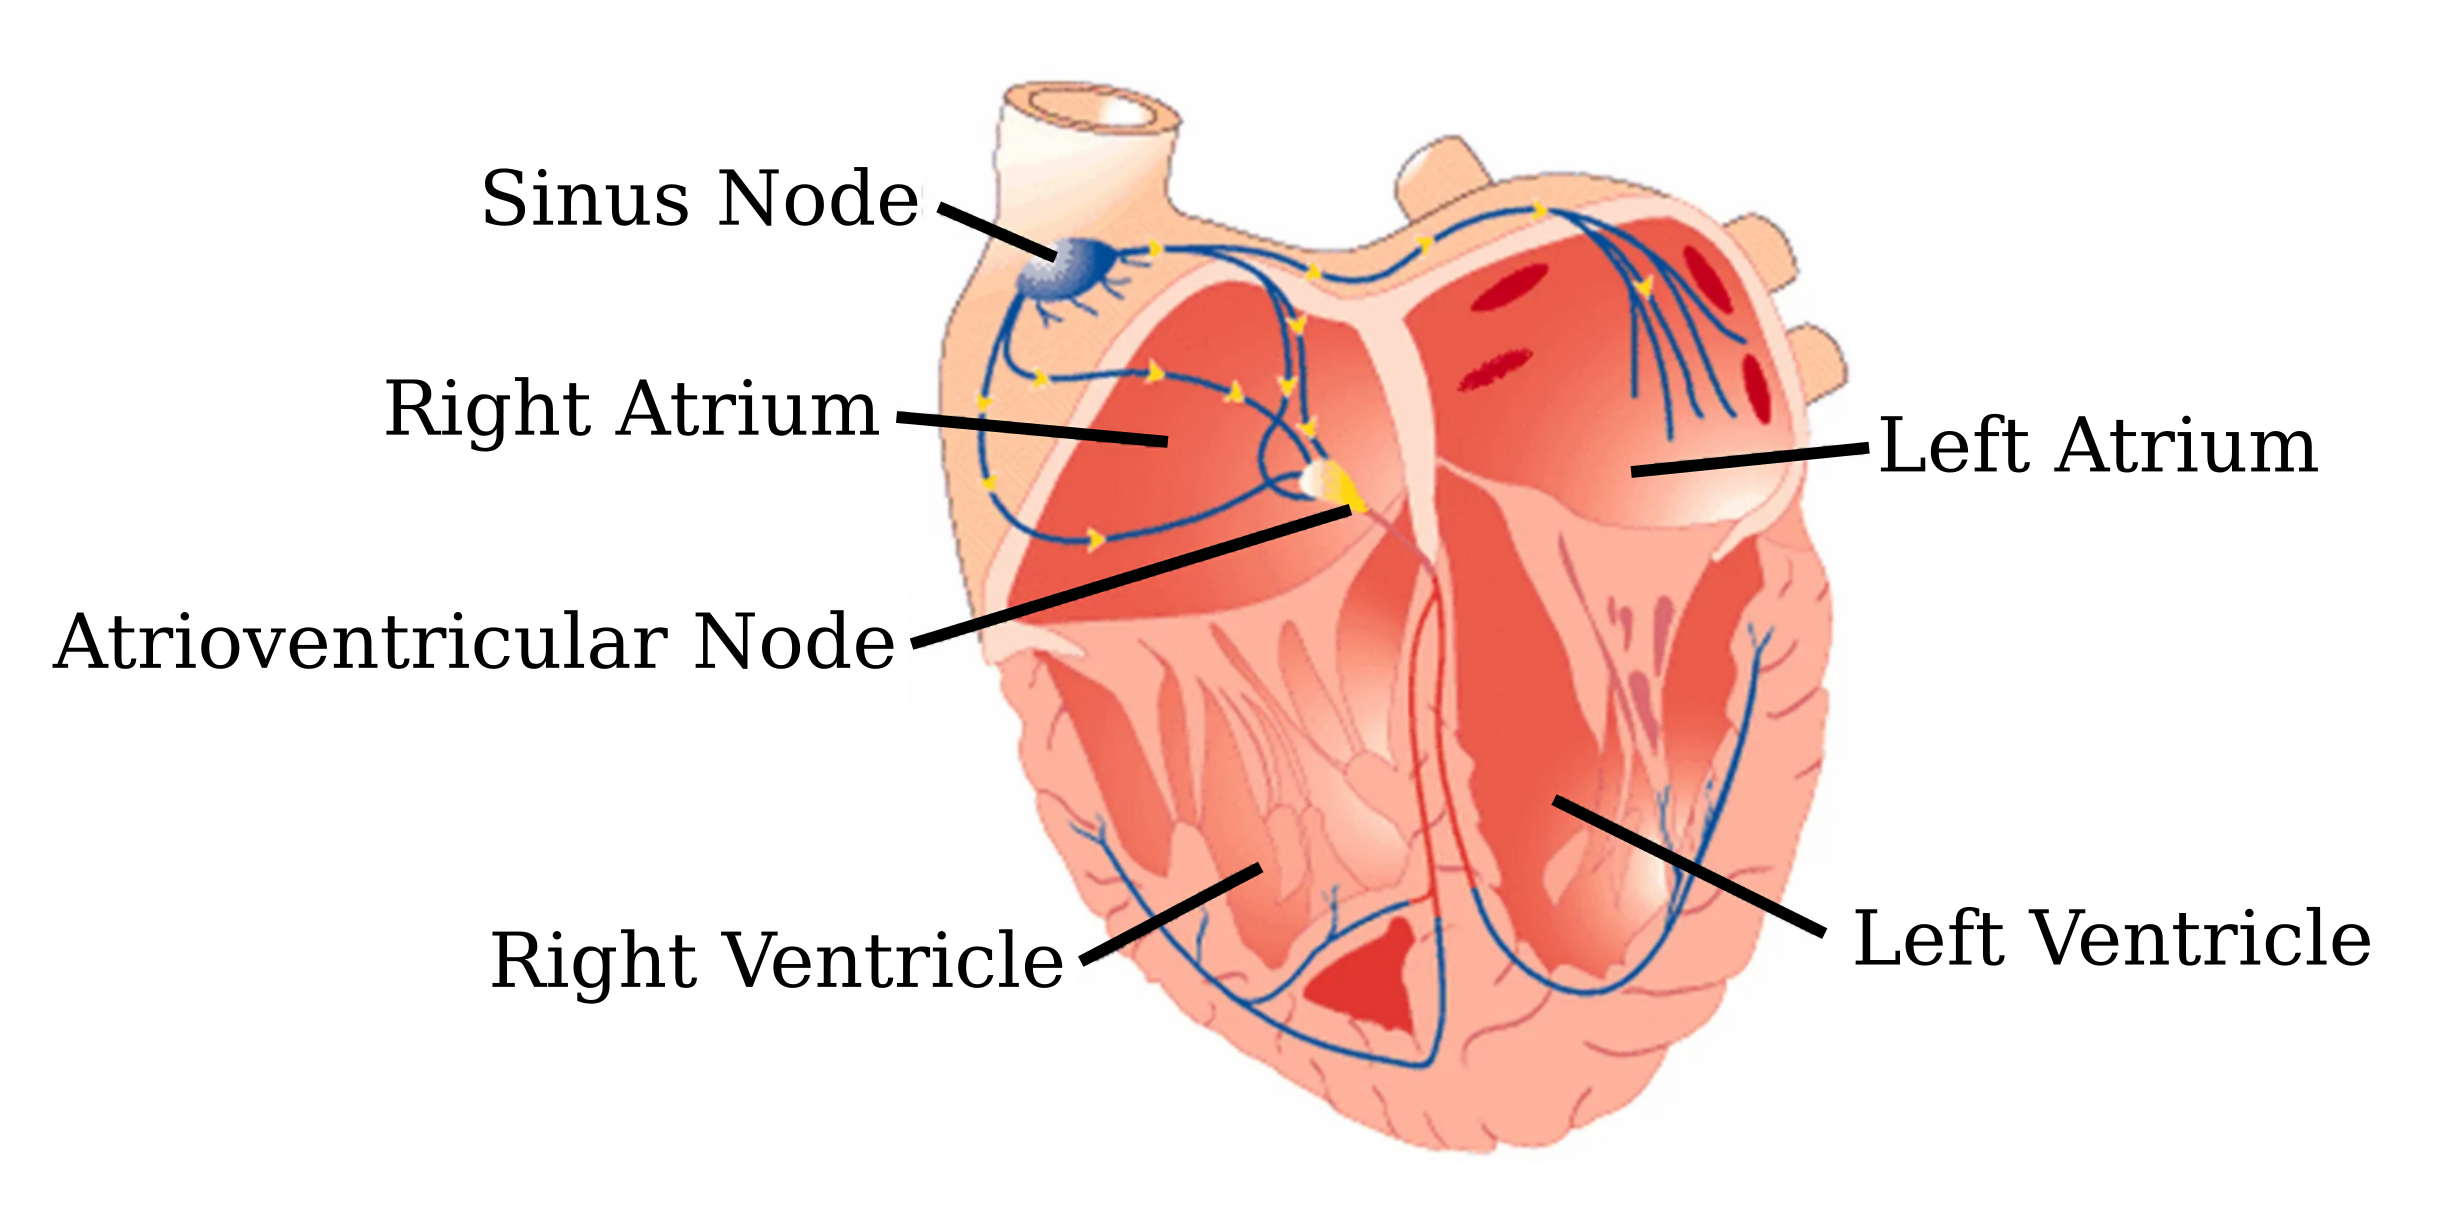
\includegraphics[width=1.0\textwidth]{figures/heart_physiology.png}
	\caption{Anatomy of the heart with the four chambers (two atriums and ventricles) including the sinus and atrioventricular node. Copyright 2019 by a-fib.com}
	\label{fig:heart_anatomy}
\end{figure}

\subsubsection{Electrophysiology of cardiac cells}
% Signalweiterleitung
% 
The action potential causes the heart muscle cells to contract and transmit the signal to other neighboring heart cells. This transmission of stimuli results in a coordinated extraction of the heart in the normal state, which results in a pumping action, the heartbeat.

% Signalverarbeitung 
% 1. Transmembranecurrent


%Cardiac cells (cardiomyocytes) are the smallest functional unit of the heart. An electro-chemical signal propagates through gap junctions between cardiomyocytes and let them contract individually but coordinated, that the heart shows a pump effect.
%In figure (\ref{fig:cardiac_excitation}) the temporal progression of three interdependent processes are sketchily shown. The blue curve shows the action potential, a temporary characteristic deviation of the membrane potential of a cell, from the rest potential. The potential is dependent on the ion-concentration within the cell. The red line shows the Calcium transient which is indirectly responsible that the cell contracts, by activating myofilaments (proteins). The Calcium-ion channel is only one kind of multiple channels to control the potential in terms of polarization, hyperpolarization or depolarization \cite{mycardium_lecture}.
%The dotted green line shows the intensity of contraction, which is a delayed reaction of the action potential course. Their temporal dependent behavior is called excitation-contraction coupling (ECC).  On the other hand it is signaling receptors\footnote{DHPR-receptor (Dihydropyridine receptor), it is a Calcium-dependent channel and functions as a voltage sensors, for further information see \cite{woodcock_cardiomyocytes_2005}.} to prevent the cell from further Calcium-ions (Ca$^{2+}$) to get into the cell. With exchanging Calcium-ions, the cardiomyocytes 'communicate' with each other, and allow the actions potential to be transferred that they act as an electrical neighbors-wise coupled system and are able to contract coordinated.
%The action potential has a refractory period where it does not show any response to a stimulus from another cell, which lasts around 250 milliseconds, to protect the heart. This period is relatively long in comparison a nerve cell, which has a refractory period of around 2 milliseconds. 


% Cells as smallest units, explaining a bit

% 


\begin{figure}[ht]
    \center
    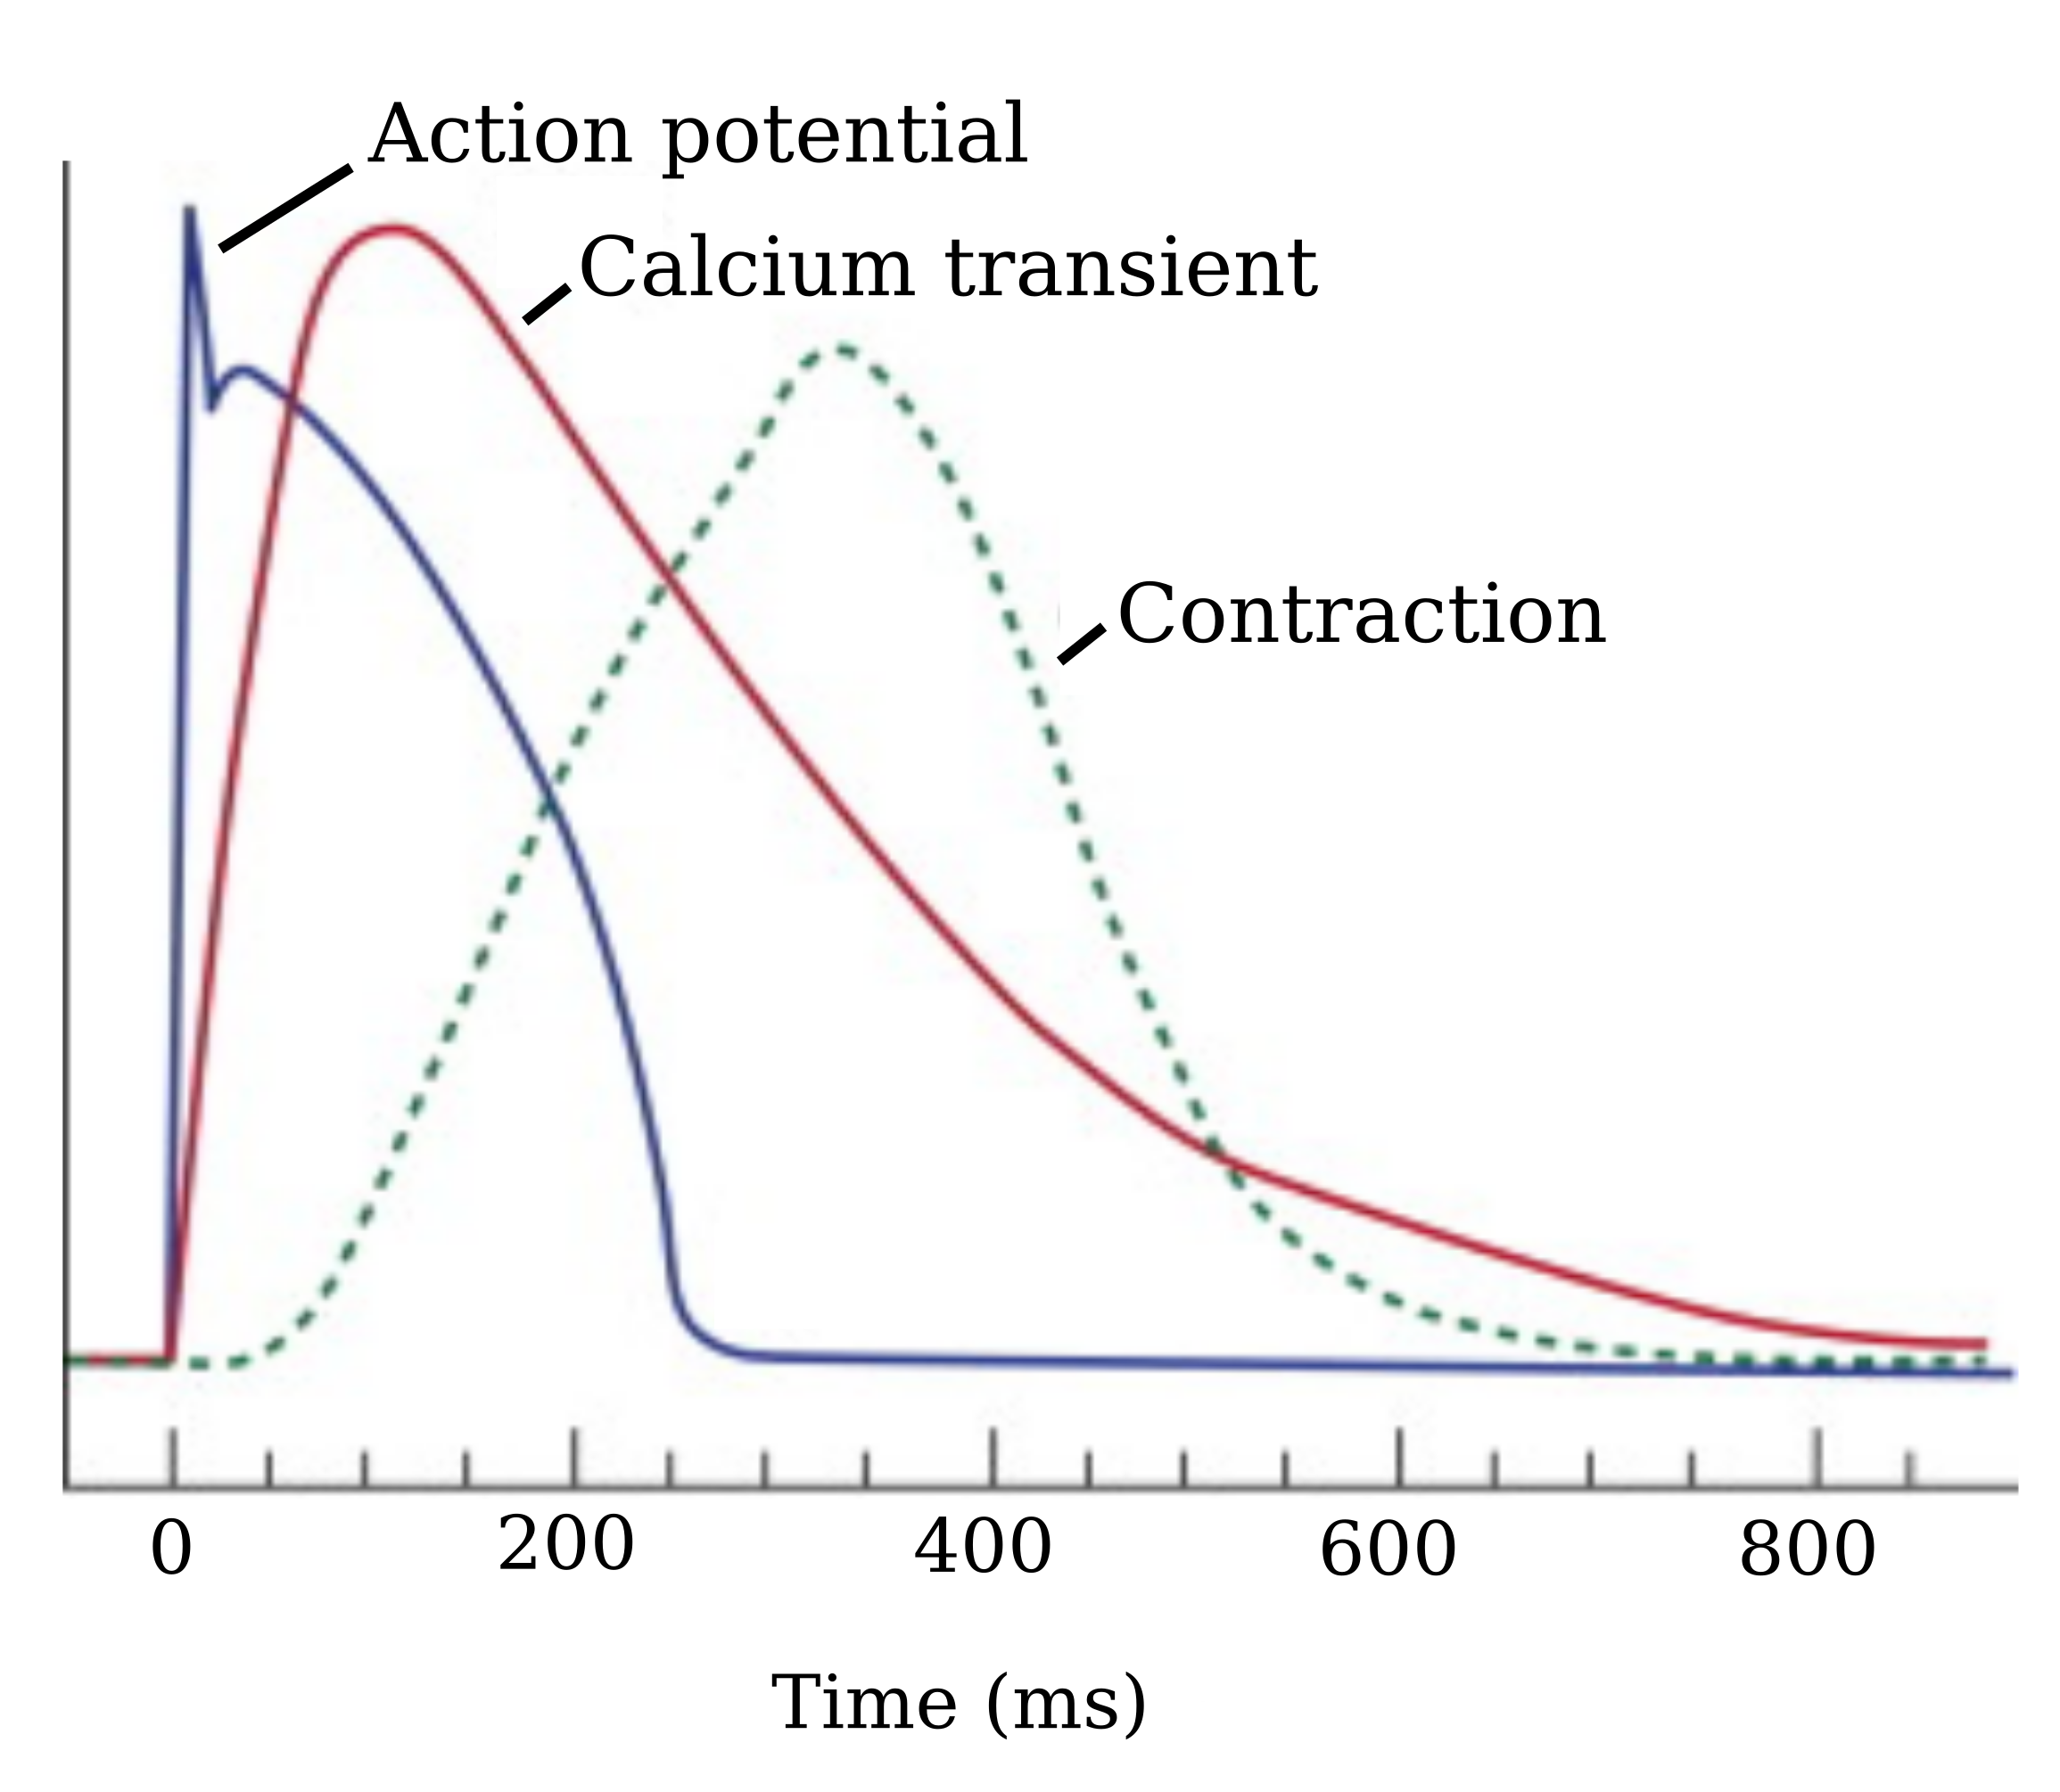
\includegraphics[width=0.7\textwidth]{figures/caradio_excitation.png}
	\caption{Physiology of the heart. Copyright 2020 by sciencedirect.com}
	\label{fig:cardiac_excitation}
\end{figure}

\section{Electrocardiography}
% In broad terms: what?
The electrocardiography is a representation of the heart's electrical activity, measured at a certain distance from the heart. The representation is in the form of potential differences, whereas the potentials are measured with the help of electrodes on the body surface. By subtracting the measurement of one electrode (or virtual electrode) with another as reference, one can gain information about the spatial potential gradient along the vector between both.
A pair of electrodes form a so called lead, by subtracting one signal from the other as a reference. A lead can be partially or fully made up of virtual electrodes, where the term virtual is used, as far as if a measurement is build from the average potential from multiple electrodes. A virtual electrode represents the potential at the spatial average of other electrodes of which it is built.
A widely known setting is the 12-lead-ECG, where 10 electrodes are used to form 12 leads. The positioning of these is visualized in figure (\ref{fig:12-lead-ecg}). The leads form vectors of which 6 lie on a vertical plane (frontal leads) and 6 on a horizontal plane (transverse leads).

\begin{itemize}
    \item Frontal leads have in common that one electrode is ideally placed (virtually) inside the heart. With the second electrode, which is marked on the image (\ref{fig:12-lead-ecg}) as V1, ...V6 (depending on the lead). The structure makes it possible to measure the potential difference between the inside of the heart and the surface of the body.
    \item Transverse leads
\end{itemize}
Here, a virtual electrode is built from \textbf{R}, \textbf{L} and \textbf{F}. It defines pairwise with V1 to V6 the first 6 leads.

\begin{figure}[ht]
    \center
    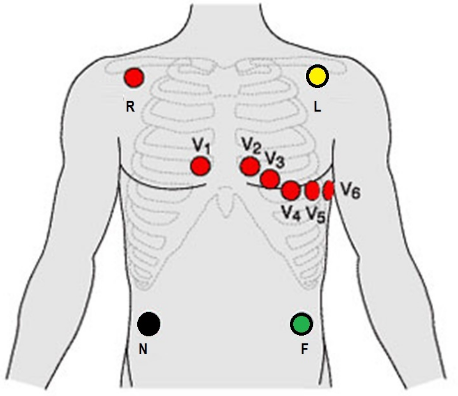
\includegraphics[width=0.7\textwidth]{figures/ecg_12_lead.png}
	\caption{\textcolor{red}{12-lead ECG, positioning. Copyright 2020 by firstaidforfree.com}}
	\label{fig:12-lead-ecg}
\end{figure}

The propagation of the electrical signals from the heart to the surface can be modeled as a diffusion process (also simulated in this work as such). This process is topic of the next chapter.
%The 12-lead ecg is designed to cover a variety of


%In conclusion, the ECG allows to measure a set of potential differences between two points at the body. By defining leads through two electrodes, a potential difference can be measured along a spatial vector. In the 12-lead ECG setting, the leads are placed such that 6 of these span vectors from the heart toward the torso. 

%The experiment as well considers though the choice of the reference electrode a 

\subsection{Forward propagation from the heart}
The terminology forward and inverse suggest that there is a direction in which the signals propagates. The suggestion here is that the potential differences lead to  
\section{The inverse problem}


\subsection{Related work and limitations}


\section{Simulation of ECG signals}\label{cap:simulation}
The following is a description of the simulation of a heart-model and its corresponding ECG signals.
The electrical activity of the heart is simulated with the FitzHughNaguro model on a pig's heart where the 3D structure is based on a computed tomography scan (CT-scan). Two grids of electrodes are placed at a certain distance from two opposing sides as visualized in figure (\ref{fig:pig_heart_in_bath}). 
The following data are considered in the numerical experiment: 
\begin{itemize}
    \item The activity of the heart model at each discrete point in the form of a system parameter (see chapter 1000).
    \item The potential differences of the respective electrodes of the grid, to a virtual electrode at the approximate center of the heart.
\end{itemize}
 

The simulation-framework is provided by Baltasar Rüchardt where the generation of the data can be divided into 4 parts, which I will describe below.\\

\textbf{1. Simulation of excitable media (electrical activity of the heart)}\\
Hey\\

\textbf{2. Reconstruction of the extracellular potential in the heart}\\
hey\\

\textbf{3. Diffusion process in the bath}\\
hey\\

\textbf{4. Calculation of the ECG}\\


%To generate ECG signals, the model for the activity in terms of extracellular potential of the heart is based on a pseudo-bidomain model. Especially when simulating an ECG the bidomain formulation is considered to be the most detailed biophysical approach \cite{bishop_bidomain_2011} but computational cost intense. To reduce the cost, the model includes the assumption, the intra- and extracellular domains to be anisotropic, but to the same degree. The bidomain model is then simplified to the mentioned pseudo-bidomain model, so that for the extracellular potential the equation 
\begin{align}
    C_m\frac{\partial V_m}{\partial t}+I_{\text{ion}}=\nabla(\sigma_m\nabla V_m)
\end{align}
applies, where $C_m$ is the membrane capacitance per unit area, and $I_\text{ion}$ is the ionic current density through the membrane. The parameter $\sigma_m$ can be regarded as bulk conductivity\footnote{For further derivation and explanation see \cite{bishop_bidomain_2011}.}.

The local ion flux is simulated with the FitzHugh-Nagumo model \cite{fitzhugh_1955}.

The 3D model of the pig-heart consists of around 32000 connective points to define a finite element mesh. The differential equations are solved with help from the open-source framework DOLFIN \cite{LoggWells2010a} in Python, the FitzHugh-Nagumo equations are solved by the implementation of the Runge-Kutta solver from scipy \cite{2020SciPy_NMeth}.

The main simulation framework is provided by Baltasar Rüchardt \cite{baltasar} and contains four steps:\\
\begin{itemize}
    \item augmented monodomain simulation,
    \item reconstruction of the extracellular potential in the heart,
    \item diffusion process in the bath,
    \item calculation of the ECG.
\end{itemize}

The potential propagates as a diffusion process through the bath, it can be regarded as a process which blurs the propagating potential. In the last step, because each electrode contains multiple points, the signal is integrated over each of these subsets. Figure (\ref{fig:pig_heart_in_bath}) shows the simulation setup with the heart inside the bath with the included ECG-electrodes, attached on the two panels from two sides.

\begin{figure}[ht]
    \center
    \hspace*{-2.45cm} 
    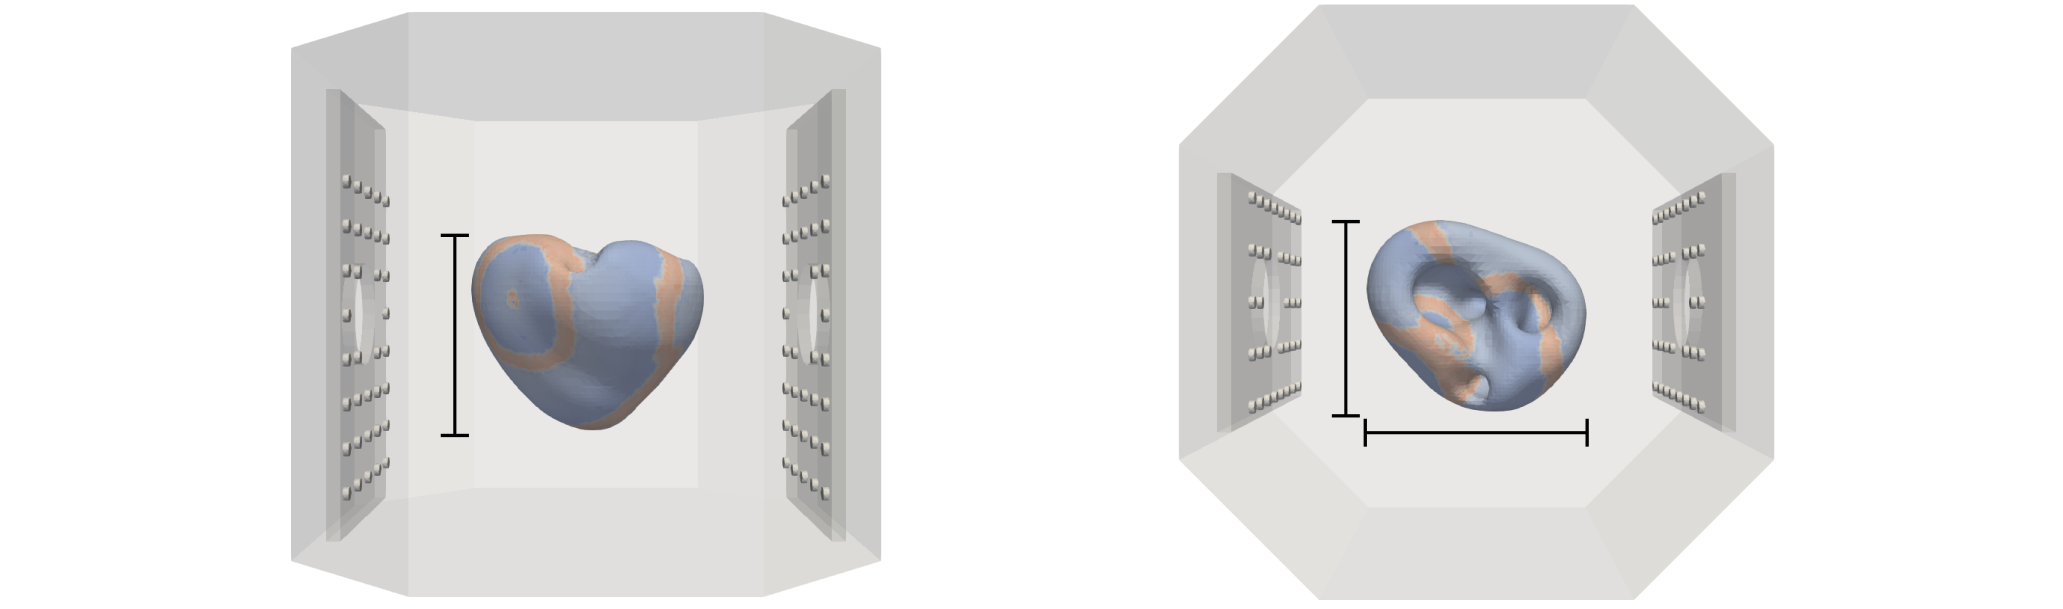
\includegraphics[width=1.4\textwidth]{figures/simulation_setup.png}
	\caption{Simulation of a pig heart, visualized with paraview \cite{paraview}, the panel on the left and right side on each image contain 64 electrodes for the simulated electrocardiography, as they are placed in the experiment in \ref{cap:concentricwave}.}
	\label{fig:pig_heart_in_bath}
\end{figure}

\section{Machine learning for iECG problem}

\begin{figure}[ht]
    \center
    \hspace*{-2.45cm} 
    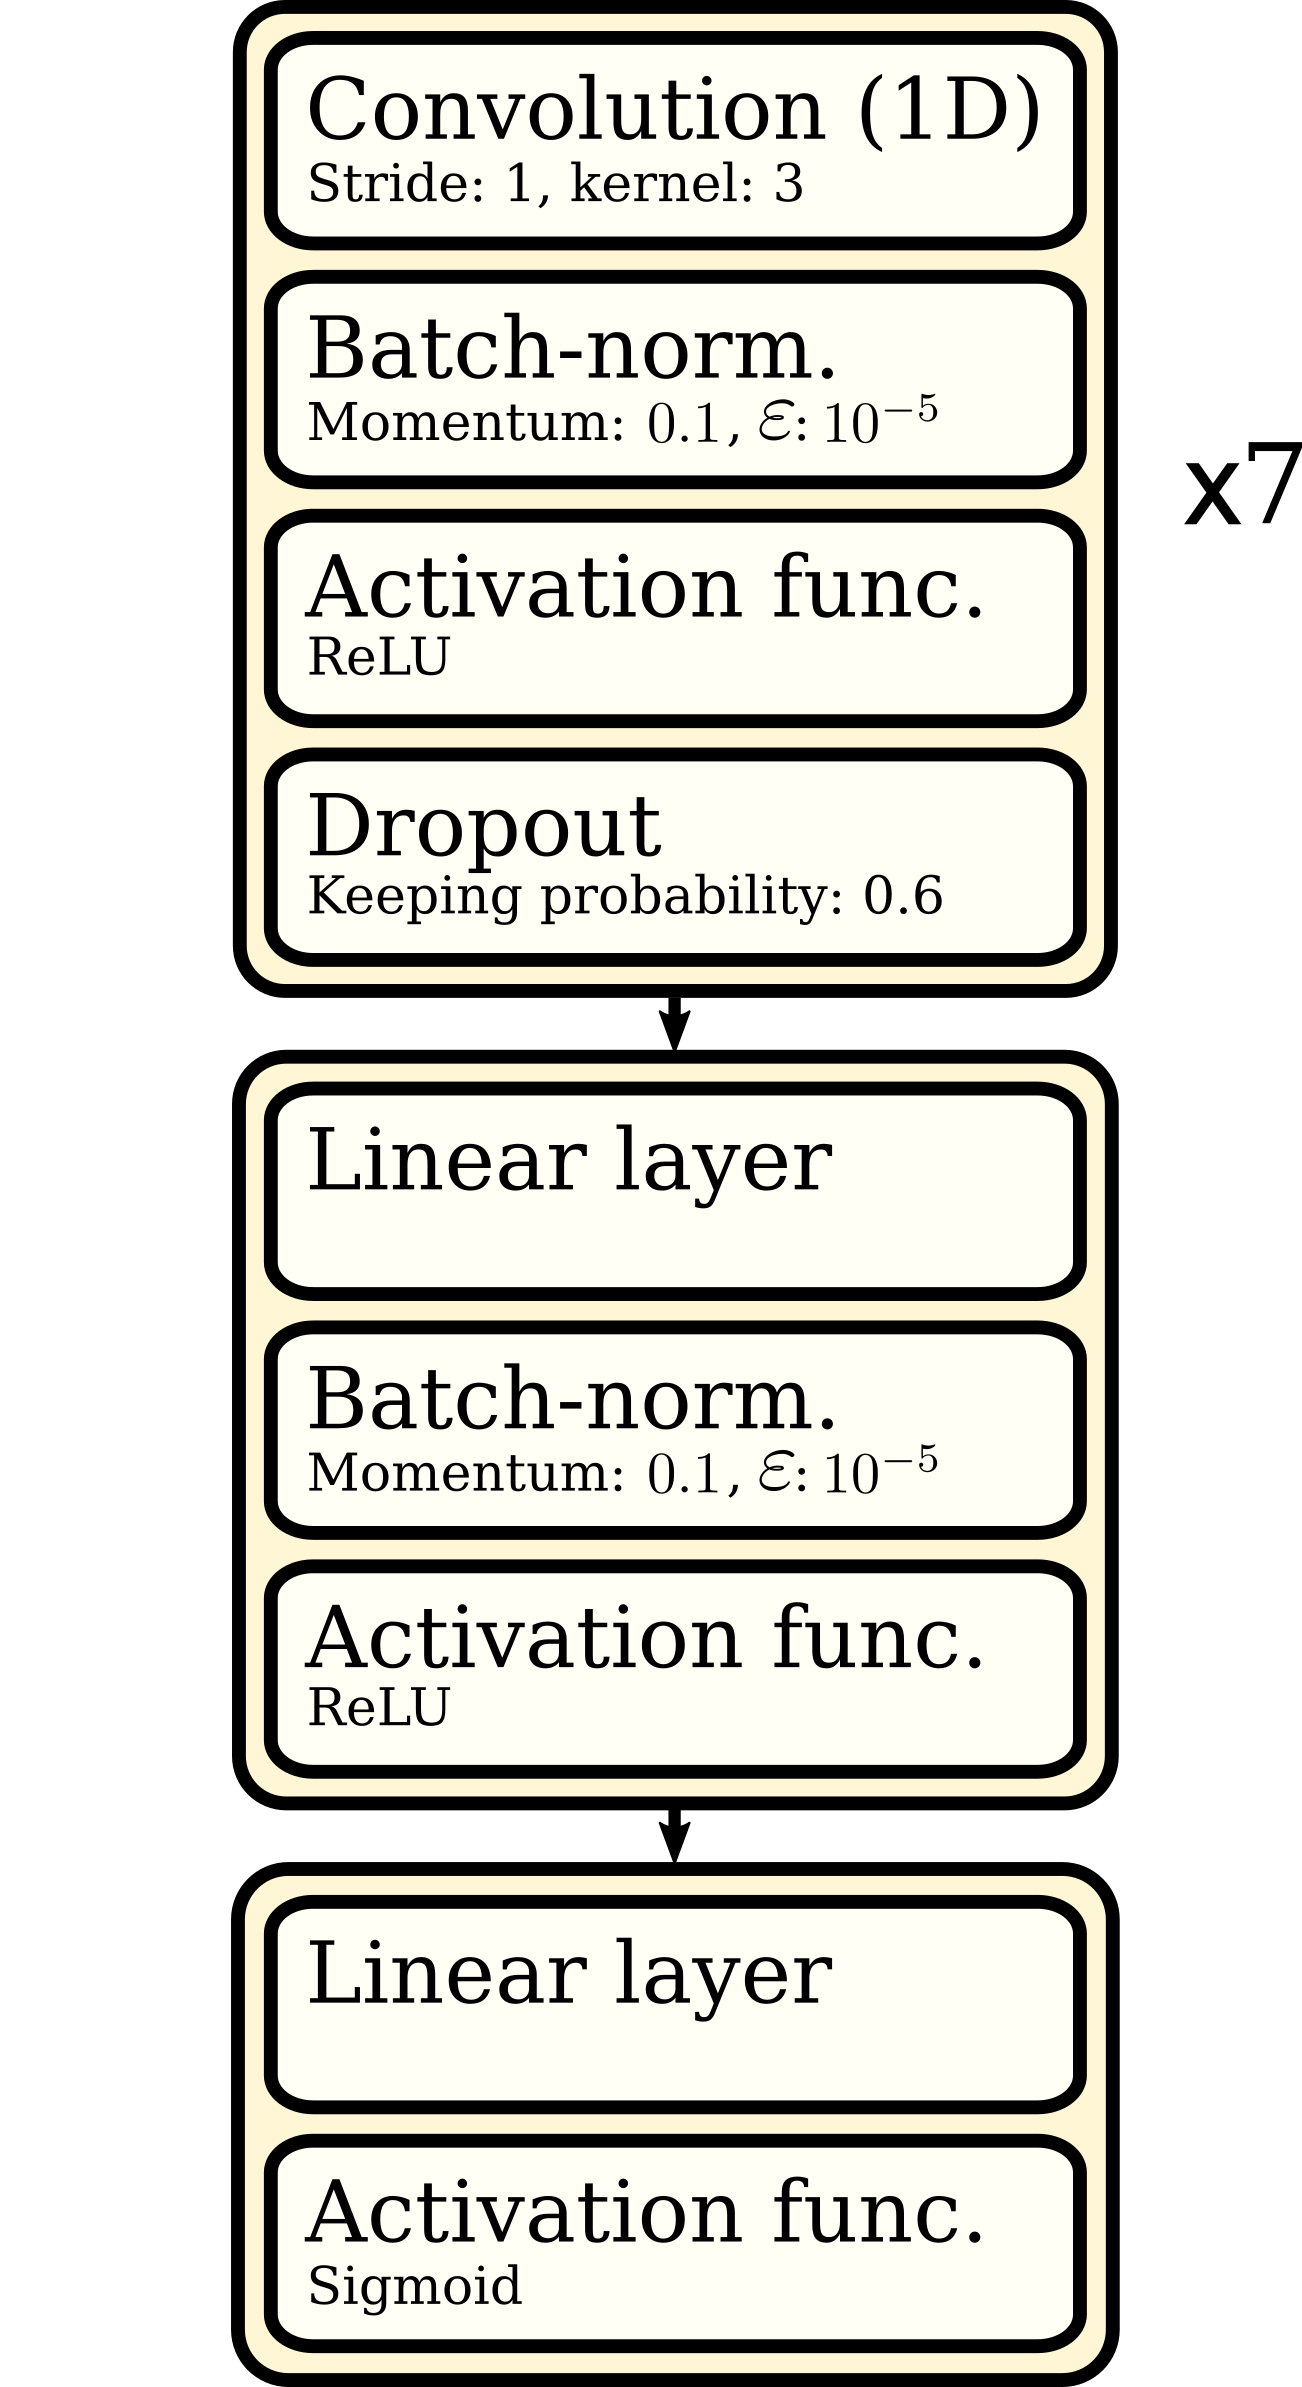
\includegraphics[width=5cm]{figures/ecg_cnn1d.png}
	\caption{}
	\label{fig:pig_heart_in_bath}
\end{figure}




\subsection{Data processing}\label{cap:processing}


\subsection{Neural network approach}

\section{Results and validation}
In the following I present the performance of the convolutional neural network (c.f. section \ref{convnet}) which is trained to predict the source of a concentric.
\subsection{Concentric Wave Localization} 
With the regularization methods during the training process (c.f. section \ref{cap:concentricwave}), the training lasted for 2310 epochs. This took around 58 minutes on a Nvidia K100 GPU. While the heart has an expansion of between around 60 and 80 length units, the model is able to predict the source of the concentric wave from the validation set on average with a displacement of 3.11 length units. Imagine a pig's heart which was simulated, and estimating the size of the heart of between 10cm and 20cm in each direction (x, y, z), the average displacement would be approximately between 0.75cm and 1cm. The comparability faces limitations due to the fact that the simulation produces a system without noise (geometrical noise in time and space, uncertainties on the measurements or positioning of the electrodes etc.) Nevertheless, it shows a first attempt that the CNN is able to localize the source of concentric waves (under the prerequisite of perfect conditions) from unknown data, whose displacement is not orders of magnitude worse when comparing with the results from the training-dataset.\\

\begin{table}[h]
    \centering
    \begin{tabular}{|c|c|}
    \hline
    training set & test set\\
    \hline
    1.74 & 3.11 \\
    \hline
    \end{tabular}
    \caption{Average displacement of the prediction from the CNN on the training- and test-dataset.}
    \label{tab:convarchitec}
\end{table}

\begin{figure}[ht]
    \center
    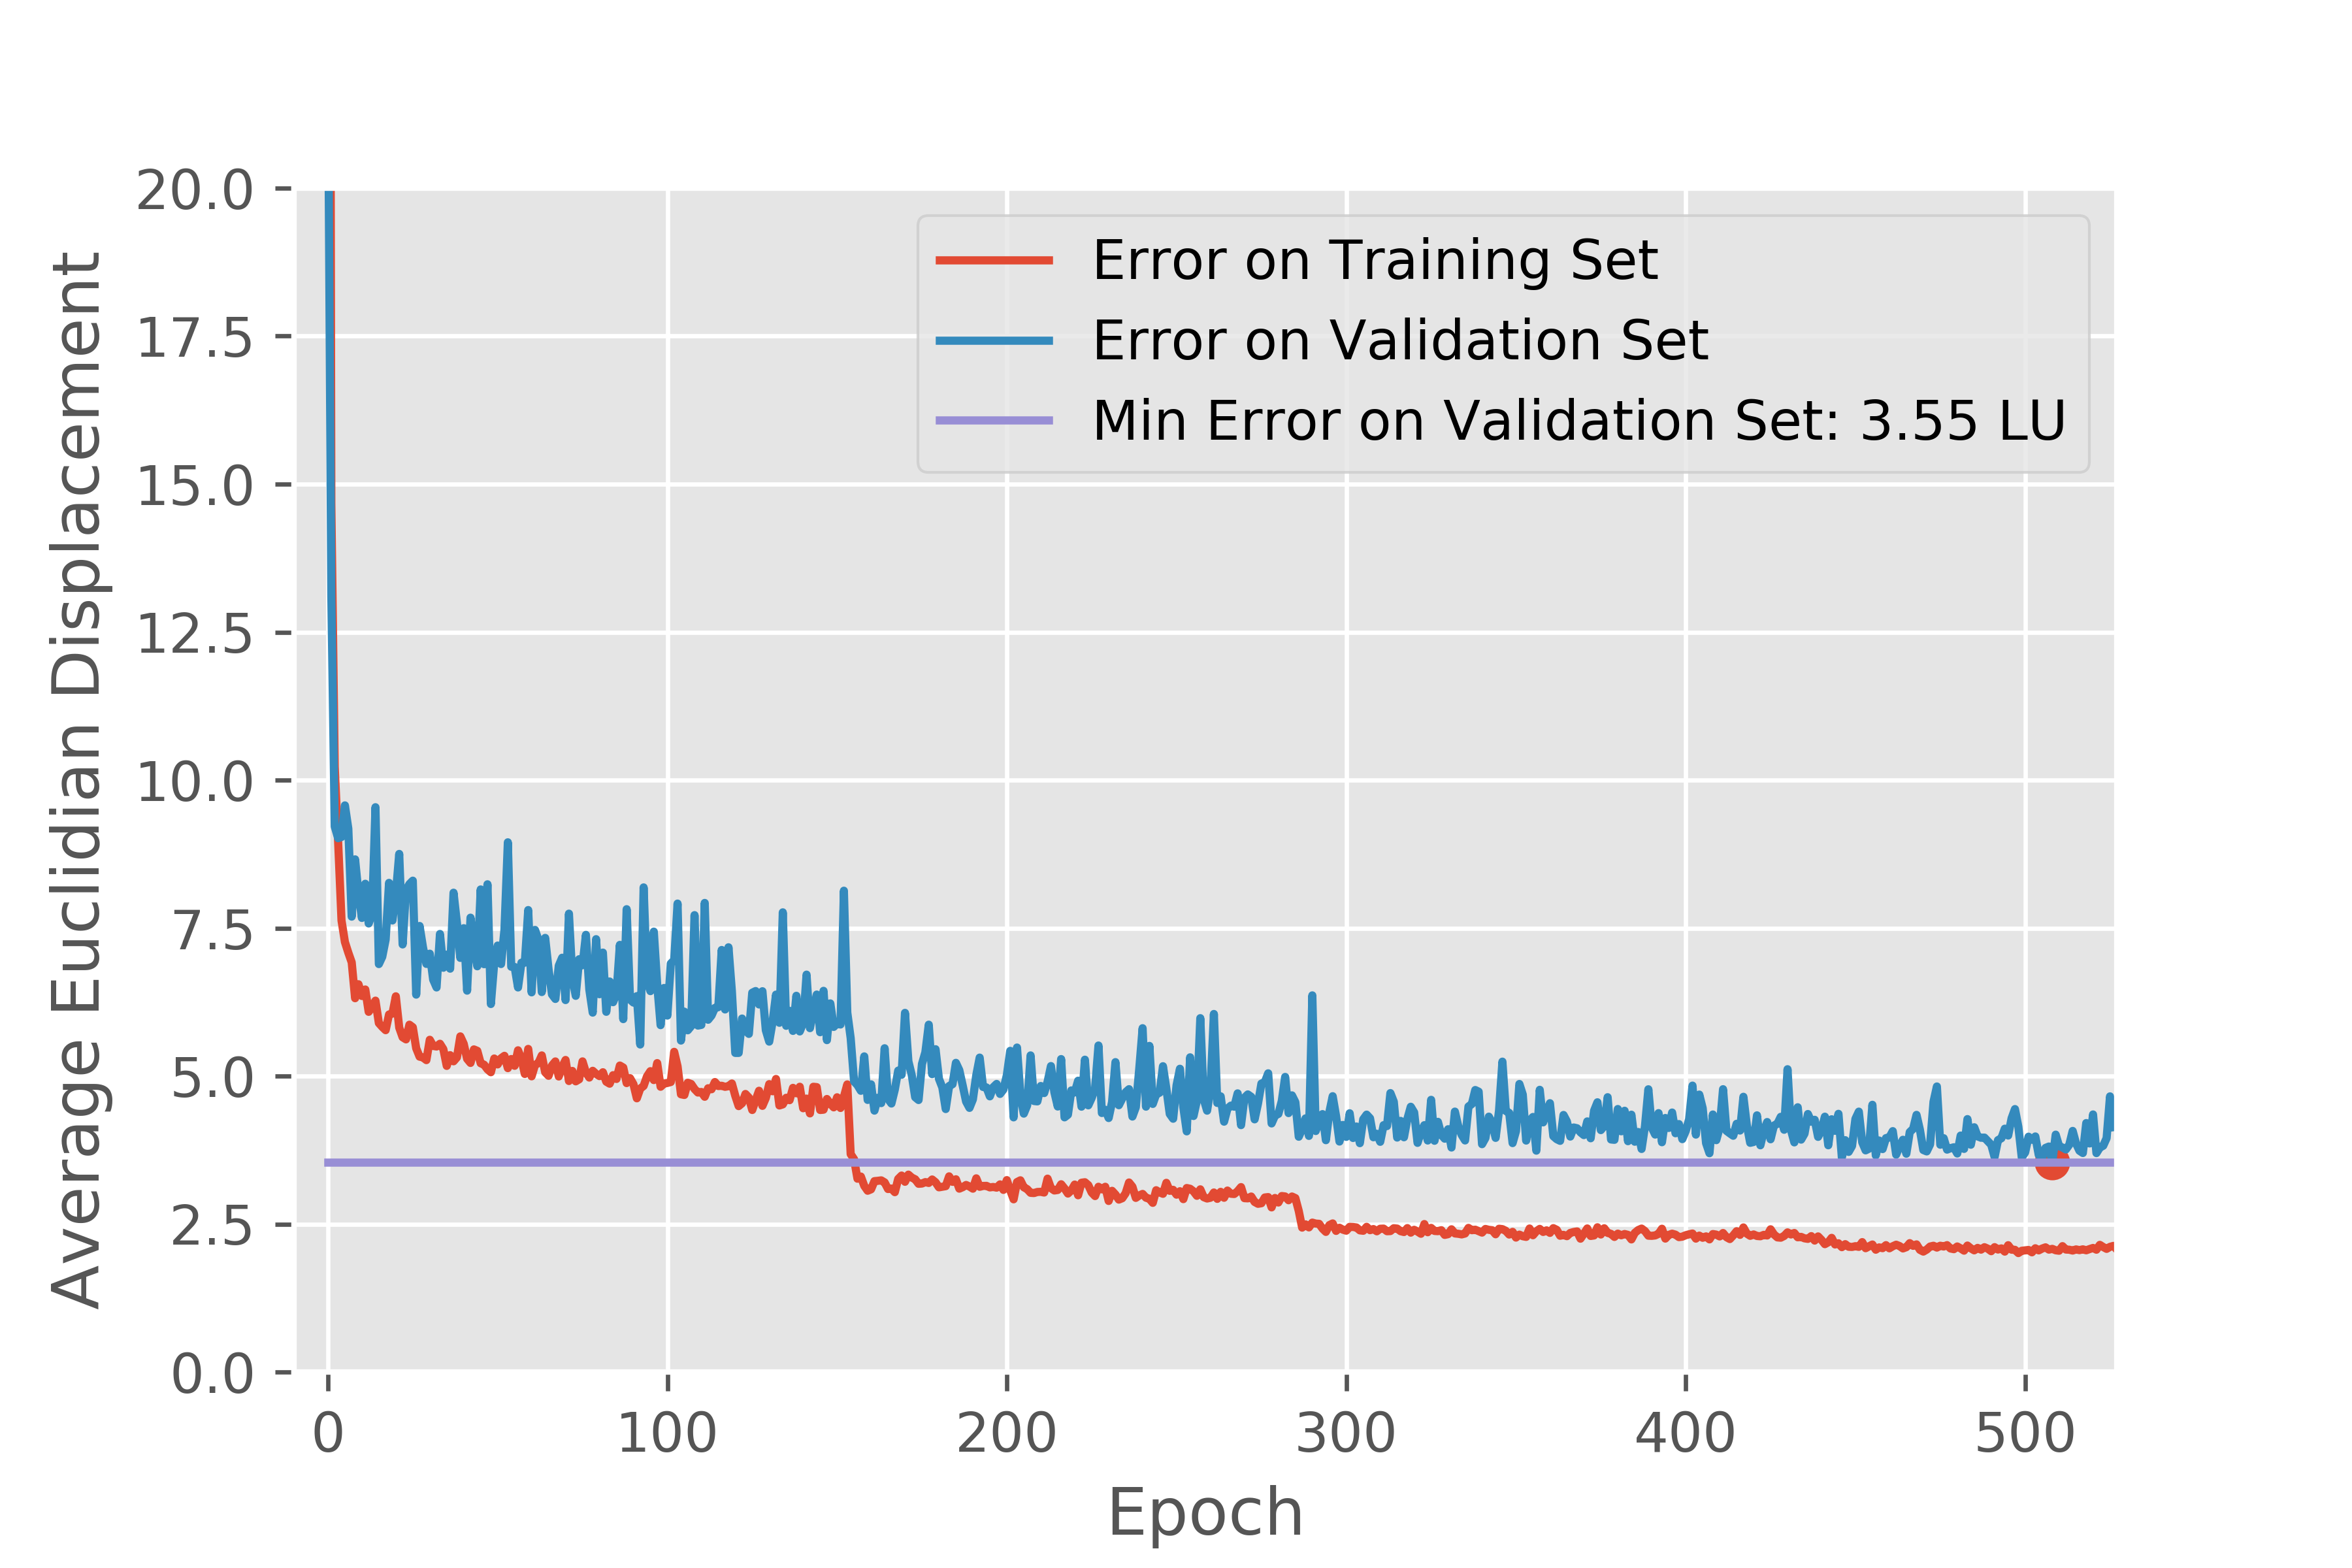
\includegraphics[width=0.99\textwidth]{figures/reg_plot1.png}
	\caption{Development of the average euclidean displacement by epoch on the training- and validation set.}
	\fontsize{3}{2}
	\label{fig:autoencoder_architecture}
\end{figure}

\subsubsection{Limitations of the Model}
This experiment is an attempt to show the principle ability to use convolutional neural network to solve a task with a time-series as input. This special posed task of the inverse problem of ECG gave comparably good results. This shows that the neural network is able to process through a temporally random selected section of fixed length, which makes it clear that it recognizes a pattern in the signals regardless of the phase of the concentric wave. The simulated heart contains of around 10000 elements on the surface, which can represent an approximate source of the concentric wave. While having 1024 simulation, having unique starting conditions, around 10\% of the available sources are already covered.  The properties of a simulation differ only in the location of the pacing events that cause the concentric wave. It is possible that some training and test simulations differ very little from each other, if the locations of the pacing events are very close to each other. In this case it may not be possible to speak of a truly unknown data set. The average minimal distance from a test-simulation to the next training-simulation is around 2.47 LU. It shows that the neural network is trained with pacing positions, which are not far distant from the test-simulations. Furthermore, the neural networks average displacement of the predictions on the test-dataset is bigger than the average distance to the next training simulation. Nevertheless, the same CNN is able to handle a dataset with additional Gaussian noise. The training on the same dataset with this noise with $\sigma=0.05$ got displacements as shown in table \ref{tab:noise}:

\begin{table}[h]
    \centering
    \begin{tabular}{|c|c|}
    \hline
    training set & test set\\
    \hline
    1.69 & 3.15 \\
    \hline
    \end{tabular}
    \caption{Average displacement of the prediction from the CNN on the training- and test-dataset, additional Gaussian noise with $\sigma=0.05$ is added to the normalized data (this means that a 5\% error is included).}
    \label{tab:noise}
\end{table}

The average displacement on the test-dataset did not increase much (a difference of 0.04LU).

    %\chapter{The inverse Problem of ECG}
In this chapter I will firstly give a short introduction of the biological background, which makes it possible to measure a potential difference between two electrodes on the torso surface. As the heart with its electro-chemical activity dominates these measurements, I will give a short overview over the anatomy and give an insight into the hearts smallest functional unit, the heart muscle cells. Furthermore a short introduction into the electrocardiography is given, TODO
%keys: Langendorff perfusion,
% neural networks,
% heart simulation

% Physiology:
    % Content:
        % Anatomy (Basics: heart shape, muscle, two chambers, Electrophysiology)
        % Sinus Node (Reason for heart beat, why is it beating, outer influcence affecting?)
        % Cardiomyocytes (as smallest unit and worker, basic for heart activity and following heart models
        % Activity of the heart 
            % Models: FNM, Barkley (advantages, disadvantages, better models?)
% key words:
    %sinus node, 

%\input{content/theory/physiology}

% ECG:
    % Content:
        % What is it in general?
        % History
        % The forward problem mathematically
        % The inverse problem mathematically
        % solving inverse problem via thikonov regularization and SVD
        % furthermorde: Neirest neighbor
            % including time via delay coordinates, disadvantages?

\section{Biological background}
To understand the measurements of an electrocardiography, we want to take a closer look at the dominant influence in the measurements, which comes from the electro-chemical activity of the heart. The mathematical description of the propagation of the electrical signals which are coming from the heart and are propagating through the body onto the body surface, is described as 'forward'. The forward propagation is measurable through potential differences between two electrodes on the torso. In following, I will explain the electro-chemical characteristics of the heart and its spatio-temporal behavior. In the terminology in which the mapping from the activity of the heart to a distant medium (like the torso) is described as forward problem, the inverse problem is defined as the tracing back of the activity to gain information of the heart's behavior, without directly measuring on its surface.

%\subsection{Physiology of the heart and Activity}
\subsection{Physiology of the heart}
QUELLE ANGEBEN
The heart consists of four chambers, the left and the right
atrium and the left and the right ventricle, as visualized in figure (\ref{fig:heart_anatomy}). Each ventricle represents a separate pump system, nevertheless it forms a unit whose pumping action is based on coordinated muscle contraction initiated by the sinus node. The sinus node in the right atrium initiates pacing signals with action potential. It does not only initiate the contraction, it also sets the pulse speed. The atrioventricular node (AV node) acts as an electrical gateway to the ventricles with controlling the signal propagation of electrical impulses. It ensures that the ventricles are completely filled before the signal from the sinus node initiates a contraction. An effective pumping action comes from the coordinated contraction of single cardiomyocytes. Their electro-chemical neighbor-wise communication leads to a signal which propagates through the heart muscle.

\begin{figure}[ht]
    \center
    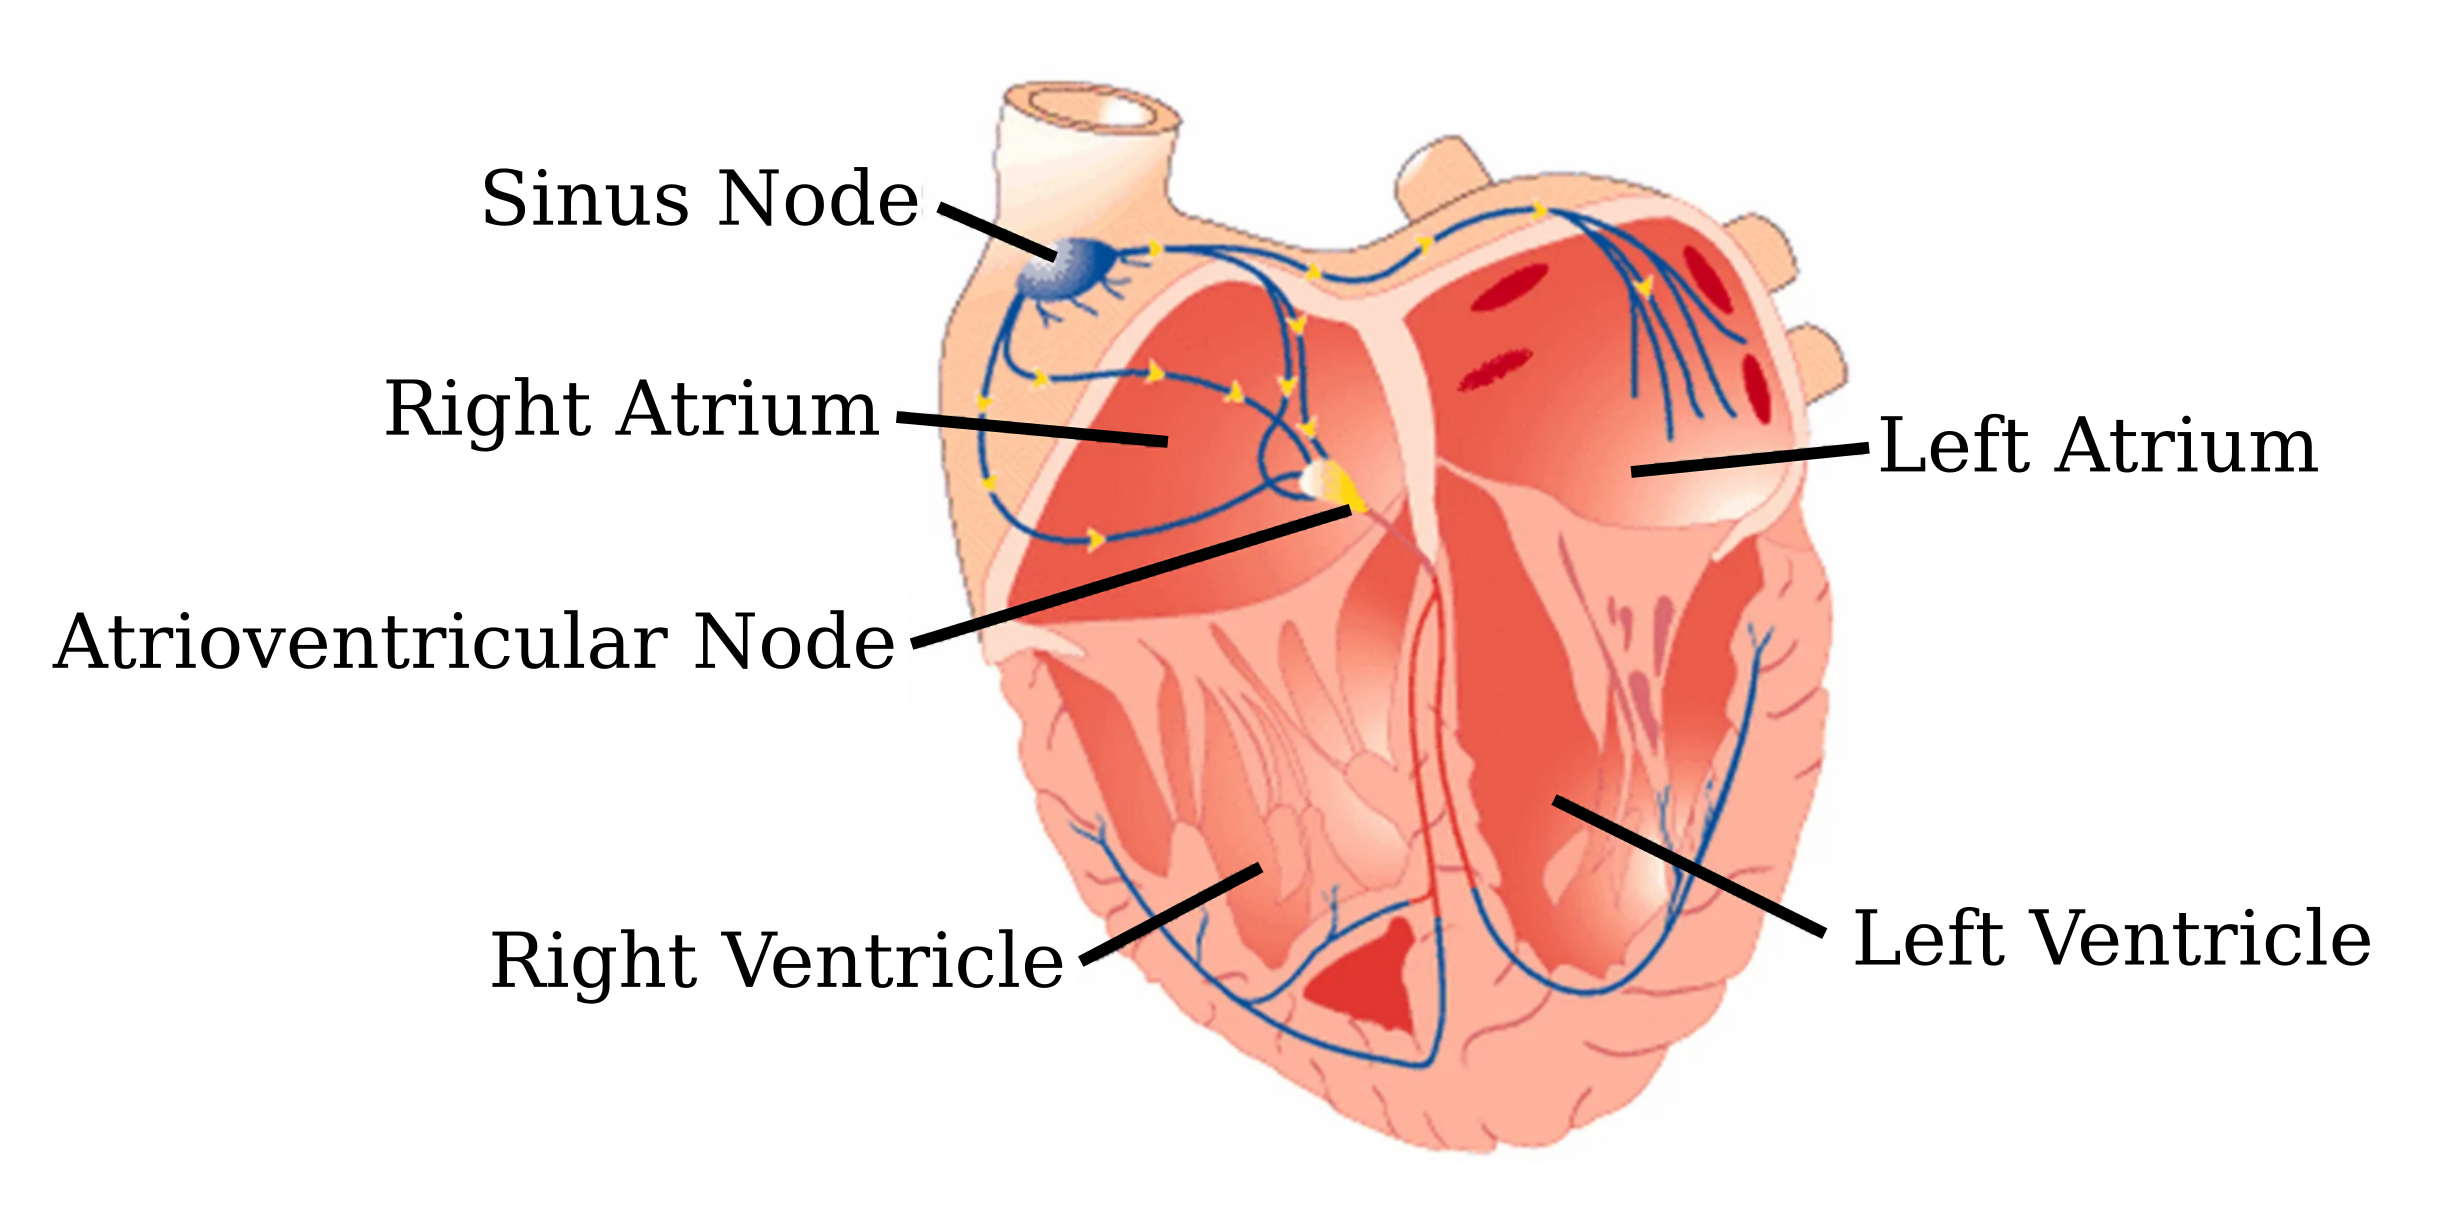
\includegraphics[width=1.0\textwidth]{figures/heart_physiology.png}
	\caption{Physiology of the heart. Copyright 2019 by a-fib.com}
	\label{fig:heart_anatomy}
\end{figure}

\subsection{Cardiomyocytes}
Understanding cardiomyocytes as smallest functional unit of the heart muscle is the key to understand the heart global behavior. An electro-chemical signal propagates through gap junctions between cardiomyocytes and let them contract individually but coordinated, that the heart shows a pump effect.
In figure (\ref{fig:cardiac_excitation}) the temporal progression of three interdependent processes are sketchily shown. The blue curve shows the action potential, a temporary characteristic deviation of the membrane potential of a cell, from the rest potential. The potential is dependent on the ion-concentration within the cell. The red line shows the Calcium transient which is indirectly responsible that the cell contracts, by activating myofilaments (proteins). The Calcium-ion channel is only one kind of multiple channels to control the potential in terms of polarization, hyperpolarization or depolarization \cite{mycardium_lecture}.
The dotted green line shows the intensity of contraction, which is a delayed reaction of the action potential course. Their temporal dependent behavior is called excitation-contraction coupling (ECC).  On the other hand it is signaling receptors\footnote{DHPR-receptor (Dihydropyridine receptor), it is a Calcium-dependent channel and functions as a voltage sensors, for further information see \cite{woodcock_cardiomyocytes_2005}.} to prevent the cell from further Calcium-ions (Ca$^{2+}$) to get into the cell. With exchanging Calcium-ions, the cardiomyocytes 'communicate' with each other, and allow the actions potential to be transferred that they act as an electrical neighbors-wise coupled system and are able to contract coordinated.
The action potential has a refractory period where it does not show any response to a stimulus from another cell, which lasts around 250 milliseconds, to protect the heart. This period is relatively long in comparison a nerve cell, which has a refractory period of around 2 milliseconds. 

\begin{figure}[ht]
    \center
    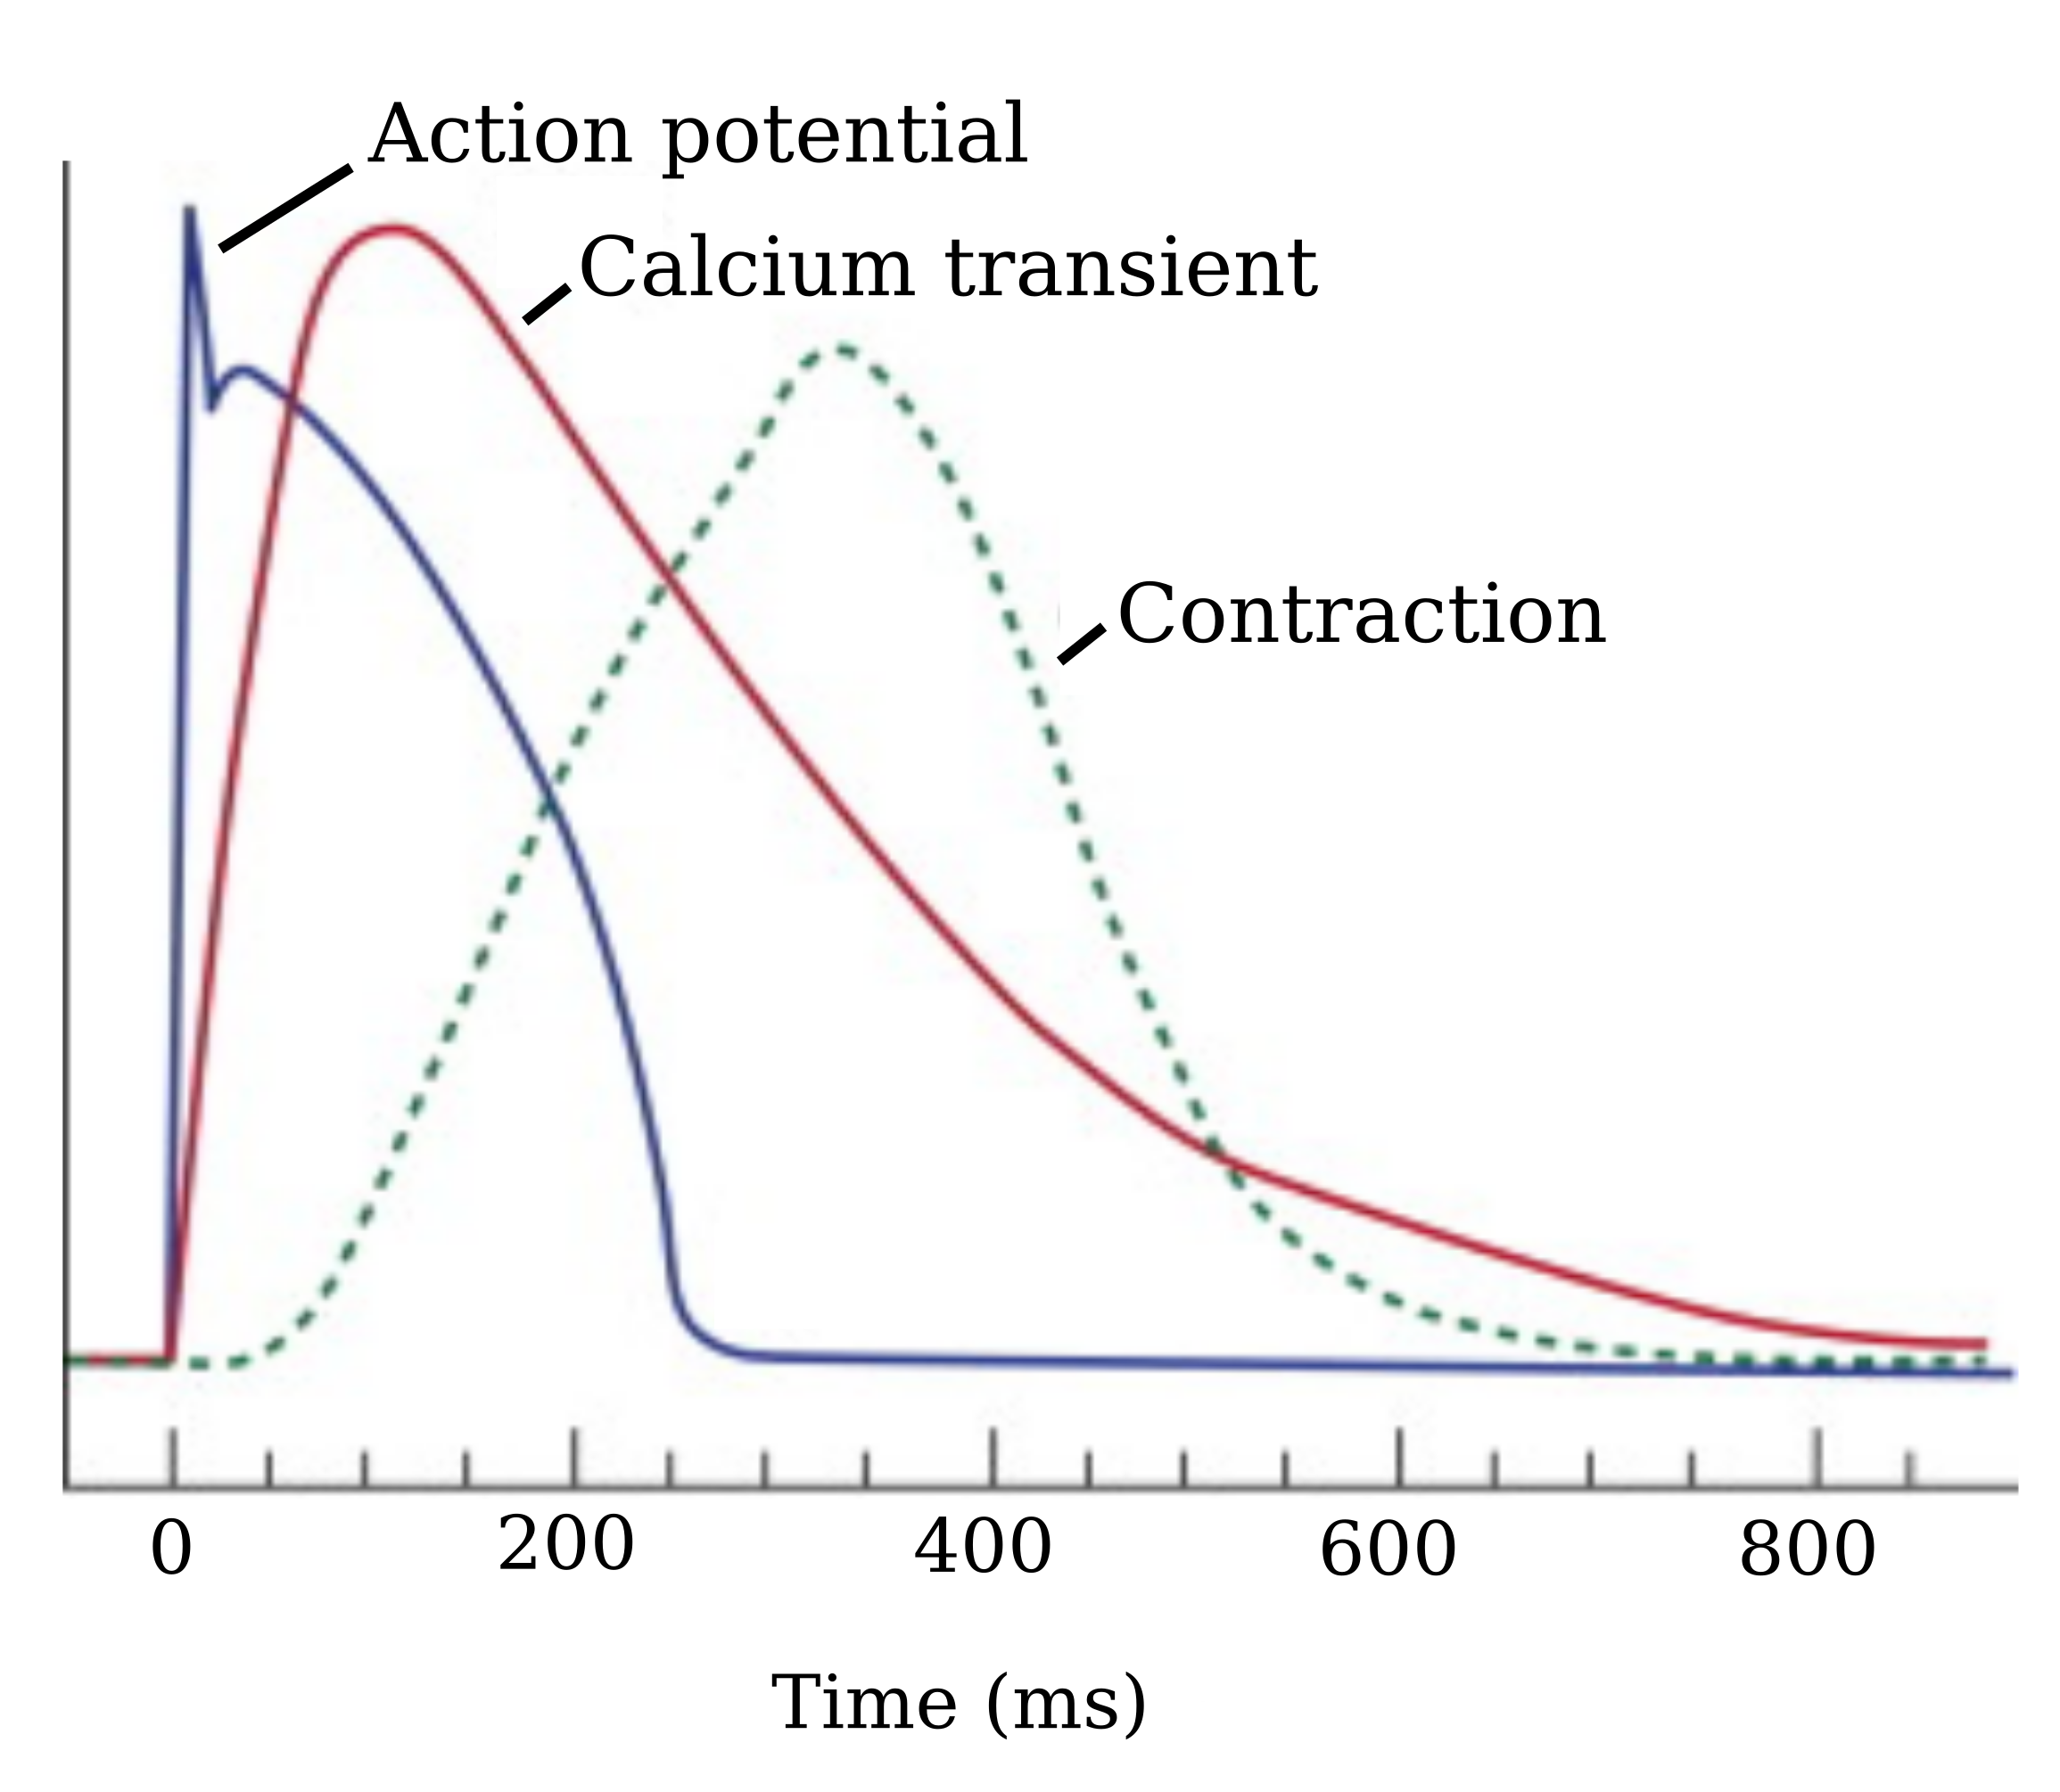
\includegraphics[width=0.7\textwidth]{figures/caradio_excitation.png}
	\caption{Physiology of the heart. Copyright 2020 by sciencedirect.com}
	\label{fig:cardiac_excitation}
\end{figure}

%\subsubsection{Activity of the heart, Arrhythmias}

%Normal sinus rhythm, spiral waves, or just chaos?

%\subsection{Models of the heart-activity}
%\textbf{The FitzHugh–Nagumo model}\\

%\begin{align}
%    \dot{v}=v-\frac{v^3}{3}-w+I_{\text{ext}}\\
%    \tau\dot{w}=v+a-bw.
%\end{align}

%The parameter $I_{\text{ext}}$ is the expression for an external stimulus. The FHN Model is a relaxation oscillator\\

%\textbf{The Barkley model}\\
%\begin{align}
%    \dot{v}=v-\frac{v^3}{3}-w+I_{\text{ext}}\\
%    \tau\dot{w}=v+a-bw.
%\end{align}
%\input{content/theory/ecg}

\section{Electrocardiography}
In broad terms, the electrocardiography can be understood as a spatial summation of the potential (blue line in figure (\ref{fig:cardiac_excitation})) of all individual cardiomyocytes after a diffusion process. Therefore, it can be regarded as the determination of the electro-chemical behavior of the heart\footnote{We will ignore possible noise from other organs like the brains which is electro-chemical active as well, nevertheless the heart dominates the ECG-signal}. The potential is measured by electrodes (non-invasive on the torso or minimal-invasive).
A widely known setting is the 12-lead-ECG, where 9 electrodes are used to form 12 leads whose potential is determined individual subtraction from other electrodes or virtual electrodes\footnote{See chapter (\ref{cap:potential_reconstruction}).}. In the following I will explain how the potential can be reconstructed in detail.
%While the forward problem, the propagation of potentials through the body, can be simulated unambiguously as a diffusion process, the inverse direction is mathematically ill-posed. 
\subsection{Potential Reconstruction}\label{cap:potential_reconstruction}
For an ECG it is necessary to have at least two electrodes which form a lead, by subtracting one signal from the other as a reference. The resulting 'normalized' signal is the spatial potential difference between them. It is also possible to form 'virtual' electrodes by taking the average of multiple electrodes. A standard lead-system is the already mentioned 12-lead ECG, its signal is based on a defined electrode positioning as shown in figure (\ref{fig:12-lead-ecg}).

\begin{figure}[ht]
    \center
    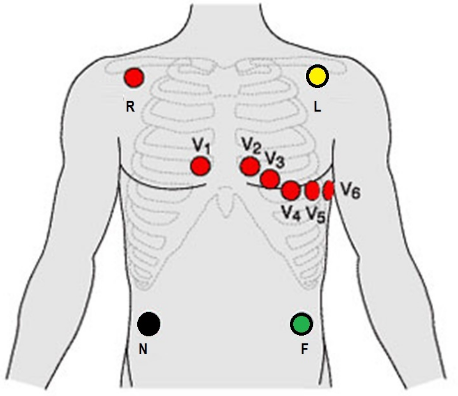
\includegraphics[width=0.7\textwidth]{figures/ecg_12_lead.png}
	\caption{12-lead ECG, positioning. Copyright 2020 by firstaidforfree.com}
	\label{fig:12-lead-ecg}
\end{figure}
By subtracting the measurement of an electrode with another reference- or virtual electrode, one can gain information about the spatial potential gradient along the vector between these electrodes. The signal of each electrode of $V$ calculates its potential by subtracting with the virtual electrode, defined by the average of $R$, $L$ and $F$ \cite{12lead_ecg}.

\subsection{History}
While the 12-lead ECG is a widely used technique on modern medicine, in the history of ECG, Einthoven was able to identify various cardiac arrhythmias with a setup, based on three electrodes, which is known as Einthoven's triangle\cite{conover_understanding_2003} (see figure (\ref{fig:einthoven_triangle}).
This setting improved the first ECG for human in 1887 by Augustus D. Waller \cite{waller_1887} in terms of robustness and sensitivity. Electrodes are attached on the left and right arm, and on the left leg, which are forming three leads (staying in the terminology of 12-lead ECG, one might call it 3-lead ECG). However, this approach is no longer relevant for modern medical information gathering.

\begin{figure}[ht]
    \center
    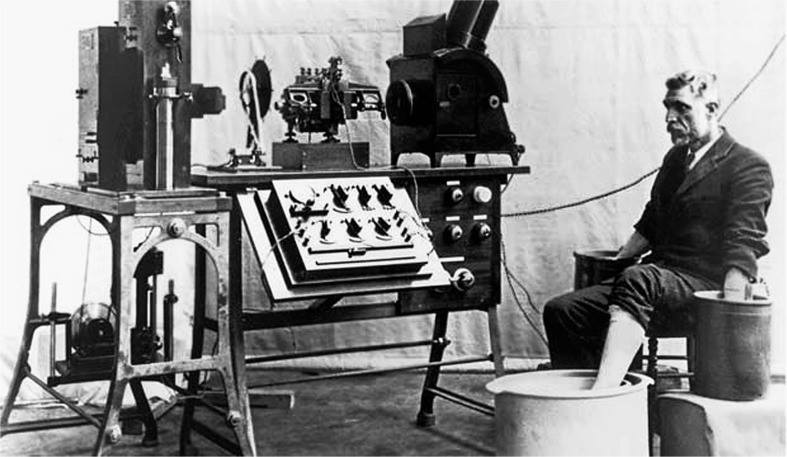
\includegraphics[width=0.7\textwidth]{figures/einthovens_triangle.png}
	\caption{Einthovens Triangle, three electrodes (left- right hand and feet) form a triangle and three leads.}
	\label{fig:einthoven_triangle}
\end{figure}


\section{Signal Propagation from the Heart}
\textbf{The forward problem}\\
The phrase forward in a dynamic system is based on the idea, that one have a known structure which emits a propagating signal 'forward' through a system. The inverse problem is therefore the tracing back of an emitted signal to obtain information about the mentioned structure and its properties.
To define a forward formulation and its relation to the inverse case, firstly we assume that the problem is linear. Existing approaches which don't consider movements of the heart through beating or breathing of a patient, are able to assume a forward propagation in a mathematical linear manner\cite[p. 241f]{sundnes_computing_2006}. The propagation can thus be written as 

\begin{align}
    \label{eq:linearity}
    \varPhi_{\text{ecg}} =\textbf{A}\cdot\varPhi_{\text{heart}}.
\end{align}

In this notation, $\varPhi_{\text{heart}}$ is the epicardial potential and $\varPhi_{\text{ecg}}$ the potential measurements of the ECG-electrodes. Both are expressed in form of a vector. Because of the linearity the forward operator $\textbf{A}$ is a matrix.\\

\textbf{Limitations of the linear formulation}\\
For simplicity we assume that there is no additional or non-linear noise, it would increase the complexity of the model and the search for $\textbf{A}$ would become even very impractical. It is not possible to include geometric noise which lead from the contraction of the heart muscles only with additional terms in a static formulation of the problem, because the contraction correlates with the excitation of cardiomyocytes with a temporal delay.
By considering the fact that there is a temporal delay between measurable excitation through the ECG-electrodes and the contraction of the muscle, one might argue that the noise from this source is not significant when the problem is not including time embedded coordinates (the temporal behavior). However, the problem arises that when time is integrated into the coordinates\footnote{Time-embedding in a linear manner is possible with delay coordinates} and the geometric noise might becomes significant noticeable.
Furthermore, in clinical measurements the movement of the torso coming from breathing, which is subject to a certain amount of random behavior, could lead to a significant noise. 
On the one hand it is possible to include the time in the linear formulation through delay coordinates, on the other hand the time-dependent geometric noise becomes increasingly relevant. Therefore, the entries of the forward-matrix with included delay-coordinates $\textbf{A}$ are not exact, also because of difficulties to define the geometry satisfying\footnote{The individual geometry of a patient's torso and its heart can be provided by for example Magnetic Resonance Imaging (MRI) or Computed Tomography (CT).}. These limitations have be considered by the assumption of a linear signal propagation for the forward problem, and the difficulty to find a good assumption for the operator might lead to practical problems. Every inverse-ECG formulation based on ($\ref{eq:linearity}$) has to face these problems, and in general the inverse mapping requires regularization methods to improve the robustness of the solution against the mentioned noise.
Regarding a biological reasonable solution as best solution of the model is also an important aspect of regularization. At the same time, with excluding possible solution it is possible that there is a loss in generalization. The solution of the problem ($\ref{eq:linearity}$) can be formulated in the question: What is the best prediction for $\varPhi_{\text{heart}}$ that the resulting ECG-signal after applying the operator $\textbf{A}$ on $\varPhi_{\text{heart}}$ is the as close as possible to the true ECG-distribution. 

%The formulation implies that the operator has to be known for the solution. In the following chapter I will introduce a $\mathcal{L}_2$-regularization method also known as Tikhonov regularization or in general Ridge-regression.
%and why the operator has to be known for this technique.

%Otherwise it might not be ignorable isn't the case if the time is embedded in the describtion of the data.

%(in clinical measurements) the movement of the torso coming from breathing. On the one hand it is possible to include the time in the formulation an therefore the temporal behavior of the dynamic and signal propagation with keeping the linearity, but on the other hand the geometric noise

%is the dominating source for the potential measurements $\varPhi_{\text{ecg}}$ of electrodes.

%$\textbf{b}$ is regarded as noise and being a vector, as well as $\varPhi_{\text{ECG}}$, holded to be the measurement (in this context ECG-signals).

\section{The inverse Problem}
In classical approaches to solve the inverse problem of ECG\footnote{Like Tikhonov regularization or Truncated SVD (TSVD)\cite{macfarlane_comprehensive_2010_page_309}.}, the forward formulation is determined first, which regularized inversion leads to a possible inverse solution. This means that the problems of the forward operator/mapping as already described, are also relevant for the inverse solution. In addition, by assuming a linear propagation, the inverse solution of (\ref{eq:linearity}) is not unique, which lead to ill-posedness.
Before giving an mathematical definition for the inverse formulation, the phrases \textit{well-posed} and \textit{ill-posed} will be introduced.  \textit{Ill-posedness} is regarded as a property from which follows that a solution cannot be given exactly. 
In the following I will show why this inverse problem is ill-posed and several state-of-the-art methods how to handle this property with regularization.

Following the definition of Jacques Hadamard \cite{hadamard_1902} a problem is well-posed if

\begin{enumerate} 
    \item A solution exists.
    \item The solution is unique.
    \item The solution depends continuously on the data.
\end{enumerate}

A problem is \textit{ill-posed} if it fails to satisfy one or multiple of these conditions, in other words if it is not \textit{well-posed}.\\
Even if the linearity is given, the inverse problem of ECG is still ill-posed, which means that there is no closed function of the form $\varPhi_{\text{heart}}\equiv f(\textbf{A},\textbf{b},\varPhi_{\text{ecg}})$ which maps the ECG-signal on the exact epicardial potential distribution (different potential distributions can lead to the same ECG-signal). It is not necessarily given that the matrix is squared and regular, which is the reason why there is not reliably a solution given by the assumption that the matrix is invertible. While the problem is not solvable in an exact way, the task leads to the search of the most probable source of the ECG-potential. To give a biologically realistic prediction of the inverse problem despite this property, there are various regularization methods which will be introduced in the following chapter.\\


\section{Common Regularization Techniques, State of the Art and Limitations}
The ultimate goal for the inverse problem of ECG would be to map the whole epicardical potential distribution based on the electrocardiogram, it is clear that this goal is utopian, but biological models can already produce relative accurate results. 
In the following, I will discuss two models that represent a regularization of the linear model. Nevertheless, these methods do not offer solutions based on biological knowledge, but only rely on empirical measurements.

The approaches for non-invasive inverse potential mapping through electrocardiography can be defined after Matthijs Cluitmans et al. \cite{cluitmans_noninvasive_2015} from 4 assumptions they make or models they use:

\begin{enumerate}
    \item The cardiac source.
    \item The signal propagation through the body.
    \item The model output, being the body-surface potential via ECG.
    \item Regularization methods to overcome the mentioned problems in the inverse mapping
\end{enumerate}
This classification of approaches includes the assumption that a forward-model is necessary to solve the problem.
However, once the patient-specific forward-matrix is estimated (firstly we focus on the linear assumption of point 2.), which maps the potential distribution from the cardiac source to the body-surface potential, the formulation of the inversion of the matrix $\textbf{A}$ can be performed. In the following I will only consider a potential-based formulation\footnote{with the wave-front-formulation they are the most often used cardiac source representations\cite{cluitmans_noninvasive_2015}.} of the cardiac source, as it is the formulation-model for the following approaches in this work. Solutions, consisting of the pseudoinverse\footnote{The inverse (not pseudo) $\textbf{A}^{-1}$ is not necessarily defined.}
$(\textbf{A}^{\text{T}}\textbf{A})^{-1}\textbf{A}^{\text{T}}$ are extremely sensitive to noise and may not be able to make biologically realistic predictions for the epicardial potential distribution. In general the problem can be redefined as the minimum of the euclidean distance between the prediction of a model $\mathcal{F}$ and the true potential distribution 

\begin{align}
    \label{eq:linear_regression}
    \min&\parallel\textbf{A}\mathcal{F}\varPhi_{\text{ecg}}-\varPhi_{\text{ecg}}\parallel_2^2
\end{align}

where $\mathcal{F}\varPhi_{\text{ecg}}$ can be regarded as a fit to the data with $\mathcal{F}\equiv(\textbf{A}^{\text{T}}\textbf{A})^{-1}\textbf{A}^{\text{T}}$ as closed form for the best solution. In other words, $\mathcal{F}\varPhi_{\text{ecg}}$ is the best solution, that the forward operator would map $\mathcal{F}\varPhi_{ecg}$ as close as possible to the corresponding true $\varPhi_{ecg}$. This formulation is well-posed with the given solution model for $\mathcal{F}$, nevertheless this does not mean that the solution is biologically realistic.
A common response to this problem is regularization, giving additional information about the biological nature are a technique to adapt the inverse problem to give a more realistic solutions. It furthermore might lead to a more robust solution against noise. 
In the following I will go through a few regularisation methods.

%While the assumptions of the forward propagation are not always linear, I will use it and its regularization methods as comparison for the machine learning approach, because it is the most known assumption.
%On the other hand I will introduce a few machine learning approaches which are used to solve special posed problems of the inverse ECG like the classification of diseases. Broadly the state-of-the-art machine learning approaches doesn't consider cell-level inverse-mapping and concentrate more on the classification problem. 
%[Zittieren: Arrythmia classification, ECG-classification in general, myocardial infarction...]: Mostly detection and classification but no potential mapping.
%While the most model consider a linear forward propagation (1) as model, \\

%\textbf{Tikhonov Regularization}\\
As a standard regularization method the \textbf{Tikhonov Regularization}\cite[p. 126]{willoughby_solutions_1979} solves the problem (\ref{eq:linear_regression}), with a modified linear regression model by constraining the magnitude of $\varPhi_{\text{heart}}$ with adding a penalty term. The problem is differently formulated as 
\begin{align}
    \label{eq:linear_regression_tikhonov}
    \min&\parallel\textbf{A}\mathcal{F}\varPhi_{\text{ecg}}-\varPhi_{\text{ecg}}\parallel_2^2+\lambda\parallel\mathcal{F}\varPhi_{\text{ecg}}\parallel_2
    %\label{eq:linear_regression_tikhonov2}
    %\min&\parallel\mathcal{F}\varPhi_{\text{ecg}}-\varPhi_{\text{heart}}\parallel_2^2+
    %{\underbrace{\lambda\parallel\mathcal{F}\varPhi_{\text{ecg}}\parallel_2}_{\substack{\text{Tikhonov}}}}
\end{align}

\cite{ito_inverse_2015}. 
The term (\ref{eq:linear_regression_tikhonov}) gives a closed form for the best prediction as
\begin{align}
    \label{eq:closed_tikhonov}
    \mathcal{F}=(\textbf{A}^T\textbf{A}+\lambda\textbf{B})^{-1}\textbf{A}^T,
\end{align}
where $\textbf{B}$ becomes the identity-matrix in case of the zero-order Tikhonov regularization. Fluctuation in a high frequency, with other words on a small scale are possibly not visible on the ECG-signal due the property of a diffusion process of showing the behavior of a low-pass-filter. In other words the term for (\ref{eq:closed_tikhonov}) with $\lambda=0$ (no regularization) could lead to a solution with biological unreasonable fluctuations. Therefore, $\lambda$ has to be adjusted to ensure a better result.
More advanced methods are taking into account the temporal behavior, that the constrained solutions which are temporally close to each other, should be reasonable close in their epicardial potential distribution as well \cite{oster_use_1992}\cite{time_space_1995}. Another approach from Brooks et al. \cite{brooks_augmented_1993} augments the Tikhonov regularization and considers multiple constraints with an additional term to ensure the temporal smoothness of the solution. 

No matter how good the regularizations are, the quality of a solution is estimated by the difference between the true ECG signals and the 'practically perfect' forward calculation of this solution. Of course, the forward operator is not perfect as already discussed. Furthermore, the solution are rather of mathematical nature, and less physiologically directly justifiable and the regularizations rely on a static geometry of the unique heart and torso.

For practice for clinical applications, one could ask does it worth it the torso and heart-mapping with CT or MRI to generate a patient-unique inverse ECG. 

Finding an extended inversion model which is reliable on different types of bodies, heart shapes and slightly varying ECG-positions, may be advantageous due to possible economic or practical difficulties. We note that regularization, based on the assumption in (\ref{eq:linearity}), need the patient-specific geometric model of the whole heart and torso as well as the forward operator to find a solution for the inverse problem. 
To hide this requirement of a model, aim of this work is to find an approach which is able to 'learn' the inverse solution without any knowledge about the forward operator, just by giving the epicardial potentials and ECG-signals. 
Can we on the other hand ask a more specific question about what is going on at the heart. This could be the localization of the source of a spiral wave, which could initiate a more targeted ablation. Limits of a model with usage of methods of machine learning, which are increasingly used to find pattern in unknown data, is aim of this work.

%\input{content/methods/neural_architecture}

\section{Methods}
\subsection{Simulation of ECG-Signals}\label{cap:simulation}
The analysis of ECG signals is based on the simulation of a pig heart, the 3D structure is from a computed tomography scan (CT-scan).
To generate ECG signals, the model for the activity in terms of extracellular potential of the heart is based on a pseudo-bidomain model. Especially when simulating an ECG the bidomain formulation is considered to be the most detailed biophysical approach \cite{bishop_bidomain_2011} but computational cost intense. To reduce the cost, the model includes the assumption, the intra- and extracellular domains to be anisotropic, but to the same degree. The bidomain model is then simplified to the mentioned pseudo-bidomain model, so that for the extracellular potential the equation 
\begin{align}
    C_m\frac{\partial V_m}{\partial t}+I_{\text{ion}}=\nabla(\sigma_m\nabla V_m)
\end{align}
applies, where $C_m$ is the membrane capacitance per unit area, and $I_\text{ion}$ is the ionic current density through the membrane. The parameter $\sigma_m$ can be regarded as bulk conductivity\footnote{For further derivation and explanation see \cite{bishop_bidomain_2011}.}.

The local ion flux is simulated with the FitzHugh-Nagumo model \cite{fitzhugh_1955}.

The 3D model of the pig-heart consists of around 32000 connective points to define a finite element mesh. The differential equations are solved with help from the open-source framework DOLFIN \cite{LoggWells2010a} in Python, the FitzHugh-Nagumo equations are solved the implementation of the Runde-Kutta solver from scipy \cite{2020SciPy_NMeth}.

The main simulation framework is provided by Baltasar Rüchardt \cite{baltasar} and contains four steps:\\
\begin{itemize}
    \item augmented monodomain simulation,
    \item reconstruction of the extracellular potential in the heart,
    \item diffusion process in the bath,
    \item reconstruction of the ECG.
\end{itemize}

The potential propagates as a diffusion process through the bath, it can be regarded as a process which blurs the propagating potential. In the last step, because each electrode contains multiple points, the signal is integrated over each of these subsets. Figure (\ref{fig:pig_heart_in_bath}) shows the simulation setup with the heart inside the bath with the included ECG-electrodes, attached on the two panels from two sides.

\begin{figure}[ht]
    \center
    \hspace*{-2.45cm} 
    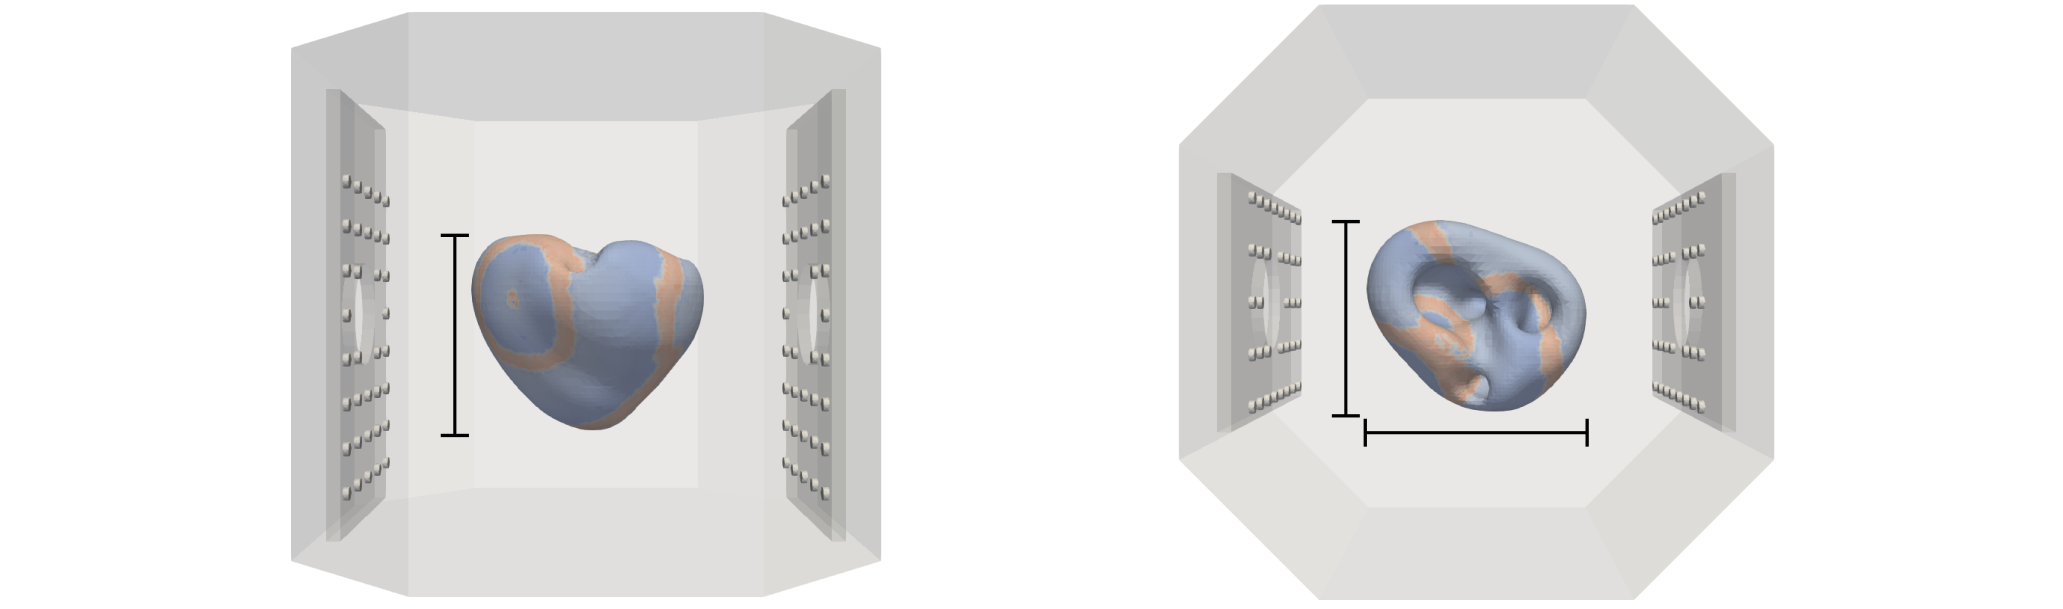
\includegraphics[width=1.4\textwidth]{figures/simulation_setup.png}
	\caption{Simulation of a pig heart, visualized with paraview \cite{paraview}, the panel on the left and right side on each image contain 64 electrodes for the simulated electrocardiography, as they are placed in the experiment in \ref{cap:concentricwave}.}
	\label{fig:pig_heart_in_bath}
\end{figure}



\subsection{Convolutional Neural Network for Concentric Wave Localization}
\label{convnet}
ECG-signals are a time series with including multiple channels. While the analysis of a time series, includes a variety on different fields like stock-market prediction, weather prediction, traffic-prediction, denoising of signals or speech analysis, a broadly used technique through these problems involves convolutional neural networks (CNN), which is also the base for the model in this work to analyse the ECG-signals. 
As visualized in (\ref{fig:cnn_architecture}) the CNN consists of seven convolutional blocks consisting of a

\begin{itemize}
    \item Convolutional layer,
    \item Batch-Normalization layer,
    \item Activation-function,
    \item Dropout layer.
\end{itemize}
Having an input of 256 time steps at 64 channels, each convolutional block is shrinking the dimension through a stride of two, by the factor of $\frac{1}{2}$, that the time-series from the input is represented after the seven convolutional block by a row of four neurons with 256 channel\footnote{The number of channel is a hyperparameter of a convolutional layer, for the exact setting, see \ref{cap:neuralnetworkarchitecture}.}. A fully connected layer follows, on which attached is a batch-normalization layer and ReLU-function, and an additional linear layer with a linear-activation function.\\

\begin{figure}[ht]
    \center
    \includegraphics[width=0.7\textwidth]{figures/neural_architecture.png}
	\caption{Basic Neural Network Architecture}
	\label{fig:cnn_architecture}
\end{figure}


\section{Experiments}
%\section{Localization of Excitation Sites from Simulated ECG}
With potential measurements from a multichannel-ECG it is impossible to estimate the exact activity of a single myocyte due to its ill-posedness. 
Nevertheless, the global activity of a heart can be influenced by single cells due to the low-resistance coupling of neighbouring cells and the resulting signal propagation. Because of this significant influence of local activity we want to explore the limits of a model, which predicts spatial information where a single heart muscle cell or a collective of cells show certain dynamic properties that significantly determine the global activity of the heart. This can be done for example by stimulating a certain small area in a periodic pattern, with the adjustment that the periodicity and strength of the pulse dominates the global activity.

In previous chapters, an attempt was introduced, which includes delay coordinates to the input of a model to solve the inverse problem. This strategy does make it possible to have an encoded information about the temporal behavior, nevertheless the spatial information, with other words the geometry of the heart is not taken into account\footnote{One have to mention that the geometry is expressed with the linear operator $\textbf{A}$, therefore the spatio-temporal behavior is indirect considered in the data set and its prediction for $\varPhi_{ECG}$}. A strategy to include this into the model, is to run a variety of ECG measurements based on the signal of the same heart respectively hearts-geometry with as different dynamics as possible. As consequence the ECG-signal contains in an encoded way the behavior of different dynamics on the same heart. 

We start with a very simple experiment to have an idea about the limits of this strategy. In the following I will introduce an experiment which realizes the mentioned steps.

\subsection{Concentric Wave Localization}\label{cap:concentricwave}
In 1024 simulations\footnote{The simulation setup and technique is explained in \ref{cap:simulation}.}, concentric waves are generated in a periodic pattern from a random point on the hearts surface, which then spread over the entire heart. The activity in each simulation is therefore significantly influenced by only one source. No sinus rhythm or a spiral wave have yet been simulated, as is the case in later experiments\footnote{These experiments are planned, see in the chapter outlook.}, that interactions between 'disturbances' and another activity can be excluded. The ECG signals thus 'see' the behavior of a continuous wave over the heart's geometry, which has a different origin in each simulation.

The goal in the first approach is to predict the source of a concentric wave, which is produced by an external stimulus $I_{\text{ext}}$ at a random chosen subset of the heart $\Omega$. The spread of this area is so small that it contains only a few elements. The signal propagates as a concentric wave through the whole heart. The external stimulus in the simulation is a function $I_{\text{ext}}(t, \textbf{s})$ which is periodic at certain area $\Omega$. It is defined as 

\begin{align}
    I_{\text{ext}}(t, \textbf{s})=
    \begin{cases}
        I_0\cdot\text{Rect}(t) & \mbox{if } \textbf{s}\in\Omega \\
        0 & \mbox{else}\\
    \end{cases},
\end{align}
with
\begin{align}
    \text{Rect}(t):=
    \begin{cases}
        1 & \mbox{if } t\text{ mod }P < d \\
        0 & \mbox{else}\\
    \end{cases},
\end{align}
where $P$ is the duration of a period and $d$ the length of the stimulus. The strength of the stimulus is given by $I_0$.\\

Therefore, the simulation setup is the same in every simulation, only the source of the concentric wave is varied. Figuratively spoken the adjustable weights $\textbf{W}$ of the neural network $\mathcal{F}_{\textbf{W}}$ which learns to identify the source of the concentric wave, learns to give an encoded expression of the globally constant settings like the geometry of the heart and the position of the electrodes or the differential equations for the spatio-temporal activity through its weights.

\subsubsection{Data Preprocessing}
Each simulation gives an output with 70 time series of length 1600 time-steps from the channels in the configuration (I) from (\ref{cap:simulation}). The first 600 time-steps are regarded as initialization-period and therefore not considered in the training process, which ensured that the concentric wave generation already shows globally influence. The potential is reconstructed by subtracting each time-series with the signal from a virtual electrodes which can be regarded as being in the center of the heart. This ensures that the spatial potential gradient is calculated in as many directions as possible. The virtual electrodes is built by the average of the four reference electrodes, visualized in figure (\ref{fig:simulation_concentric_wave_overview}).
In the next step, 80\% of the data will be used for training, the remaining 20\% for validation to ensure the generalizability of the model on unknown concentric waves sources.

\begin{figure}[ht]
    \centering
    \hspace*{-1.7cm}
    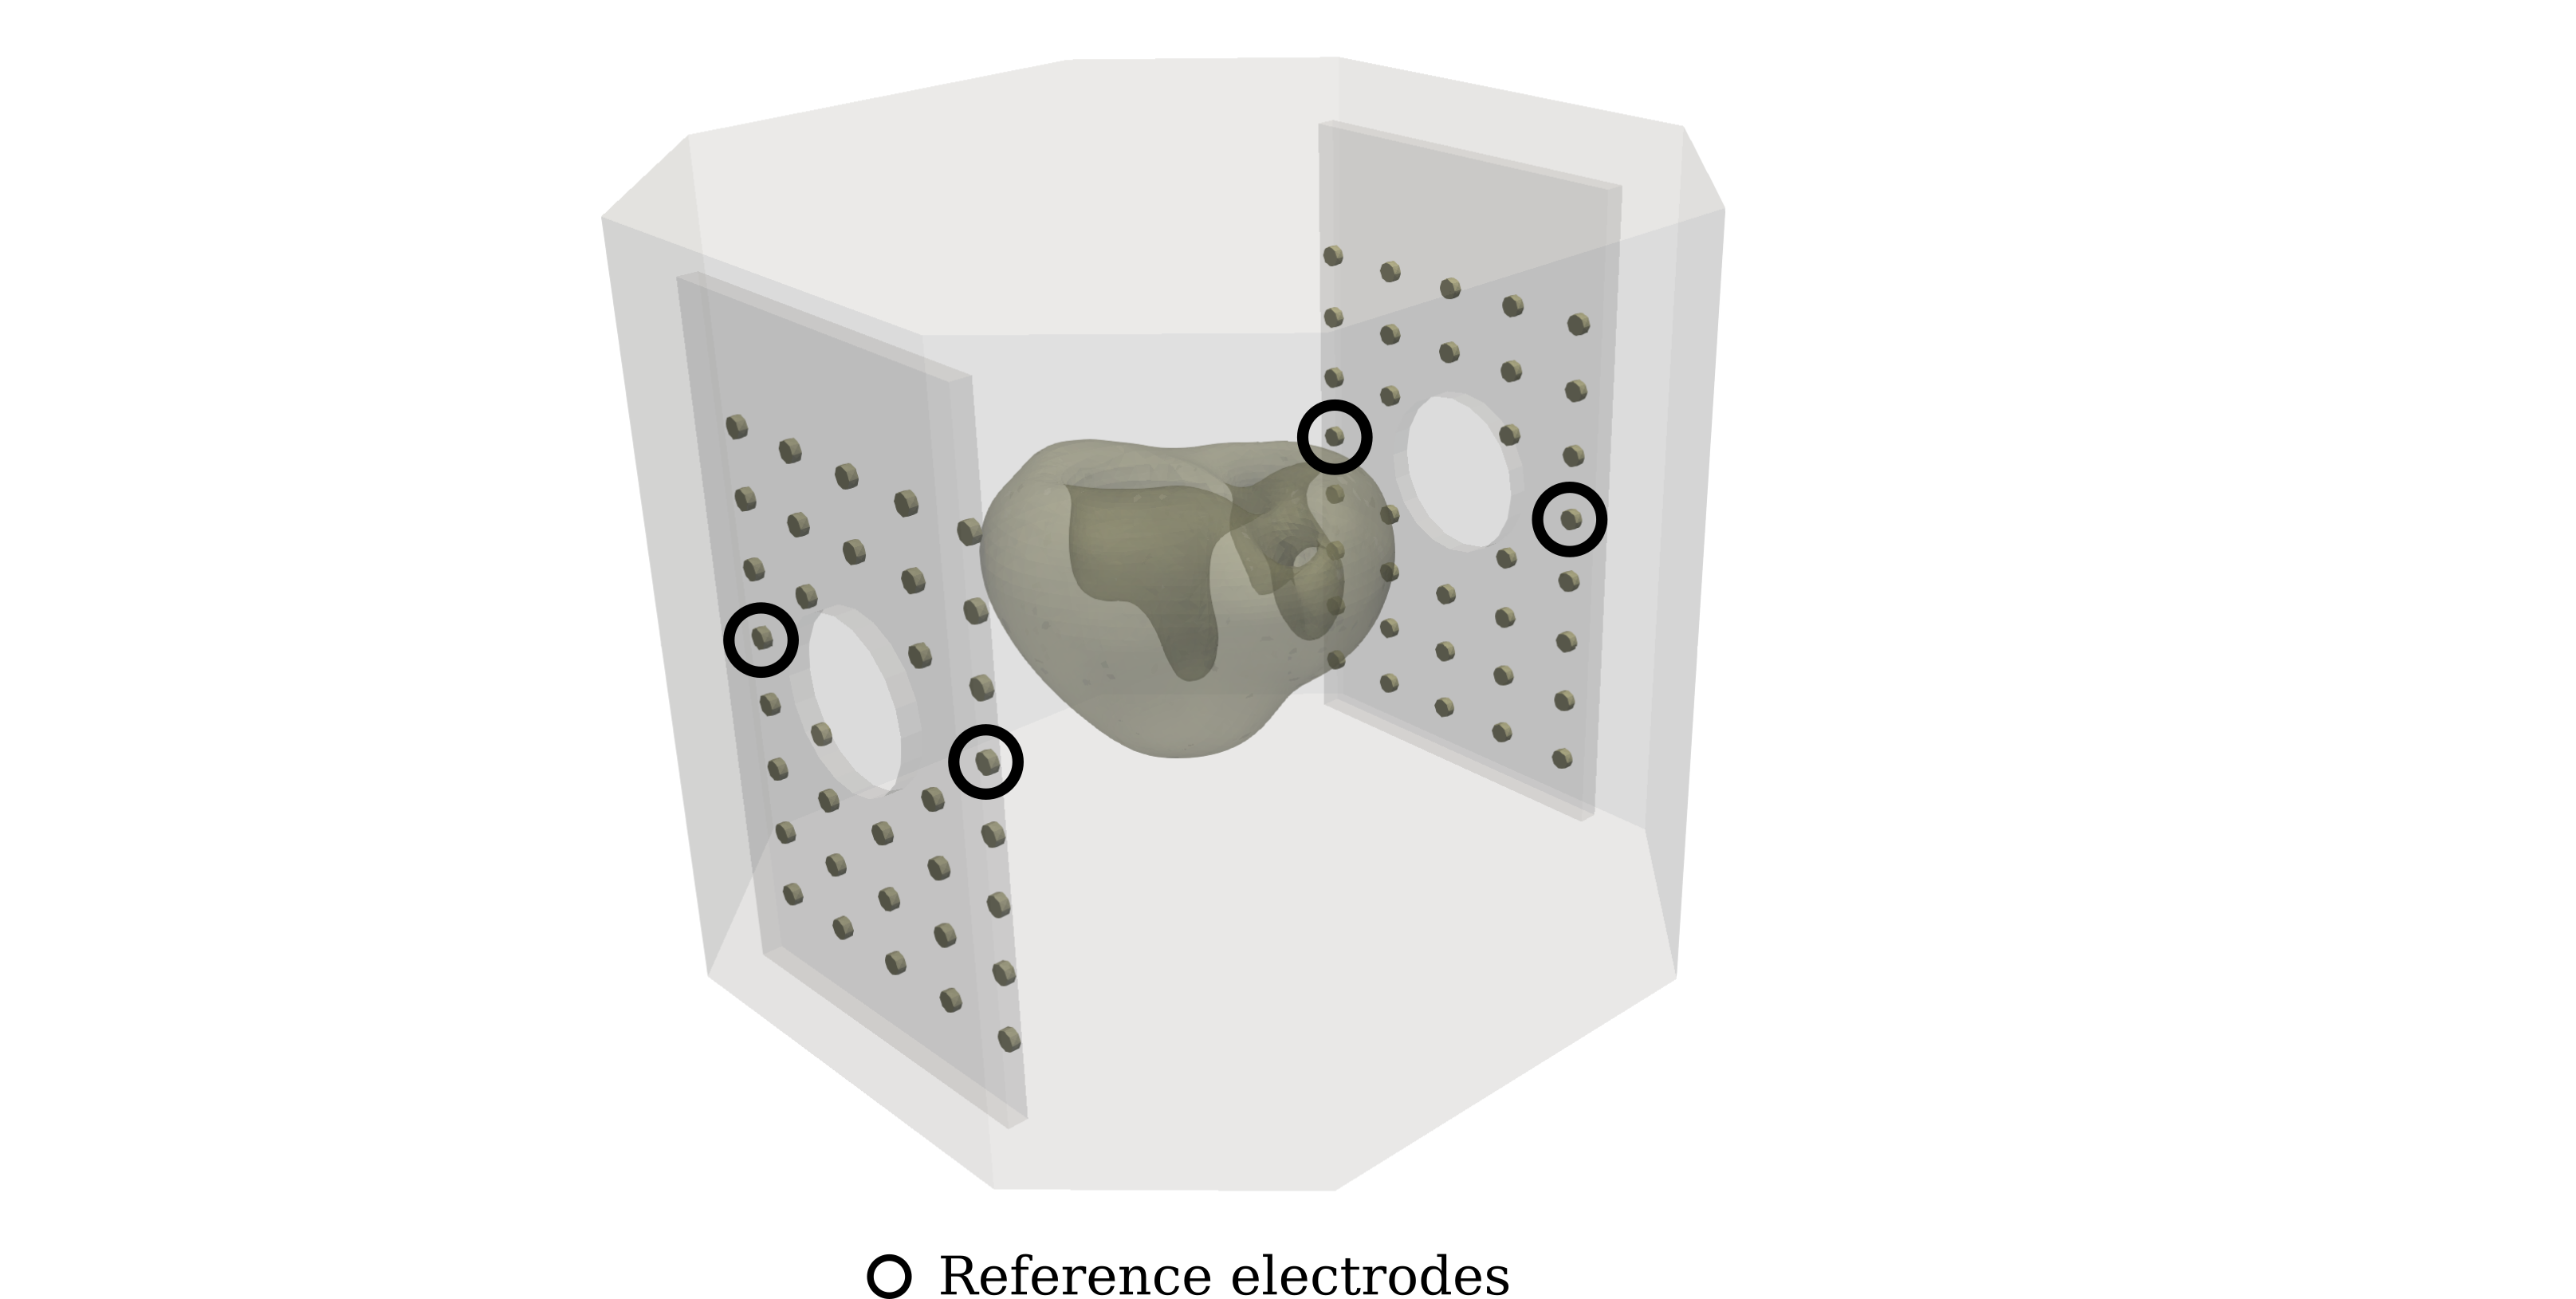
\includegraphics[width=1.4\textwidth]{figures/heart_overview_inkscape.png}
	\caption{Simulation setup with the reference electrodes (marked with black circles).}
	\label{fig:simulation_concentric_wave_overview}
\end{figure}

From the remaining 1000 time-steps on each simulation in the training- and test-set, 8 sub-sequences of length 256 are picked at random times. The simulations have an average period length of 223 time-steps, therefore the length of a single sub-sequence includes around 1.15 period-length. 

For 1024 simulation the amount of sub-sequences result into $1024\cdot8=8192$ where 6536 of them are used for training, and 1640 for testing\footnote{Because of technical problems, two simulation have been excluded, therefore 16 sub-sequences are missing.}. The choice of random starting-points comes from the idea, that the model should be invariant through time-shift in its prediction. With this property the model is able to give nearly the same prediction on different phases, without being dependent on a certain selection.\\


\subsubsection{Training-Process}
The training/optimization process is based on the adjustment of the model immanent weights. For this purpose the stochastic gradient descent method Adam (c.f. section \ref{cap:optimizer}) is used. The method does an update-step with including a batch of size 256, including random chosen samples. The hyperparameters of the optimizer are as in the tensorflow-API \texttt{keras} by default as $\alpha=0.001$ (learning-rate), $\beta_1=0.9$ $\beta_2=0.999$ and $\varepsilon=1\cdot 10^{-7}$.
During the training, after the loss did not decrease for 32 epochs (plateau-phase), the learning-rate will be decreased by a factor of 0.8. If this phase lasts longer than 256 epochs, the training will be stopped.

\section{Results}
In the following I present the performance of the convolutional neural network (c.f. section \ref{convnet}) which is trained to predict the source of a concentric.
\subsection{Concentric Wave Localization} 
With the regularization methods during the training process (c.f. section \ref{cap:concentricwave}), the training lasted for 2310 epochs. This took around 58 minutes on a Nvidia K100 GPU. While the heart has an expansion of between around 60 and 80 length units, the model is able to predict the source of the concentric wave from the validation set on average with a displacement of 3.11 length units. Imagine a pig's heart which was simulated, and estimating the size of the heart of between 10cm and 20cm in each direction (x, y, z), the average displacement would be approximately between 0.75cm and 1cm. The comparability faces limitations due to the fact that the simulation produces a system without noise (geometrical noise in time and space, uncertainties on the measurements or positioning of the electrodes etc.) Nevertheless, it shows a first attempt that the CNN is able to localize the source of concentric waves (under the prerequisite of perfect conditions) from unknown data, whose displacement is not orders of magnitude worse when comparing with the results from the training-dataset.\\

\begin{table}[h]
    \centering
    \begin{tabular}{|c|c|}
    \hline
    training set & test set\\
    \hline
    1.74 & 3.11 \\
    \hline
    \end{tabular}
    \caption{Average displacement of the prediction from the CNN on the training- and test-dataset.}
    \label{tab:convarchitec}
\end{table}

\begin{figure}[ht]
    \center
    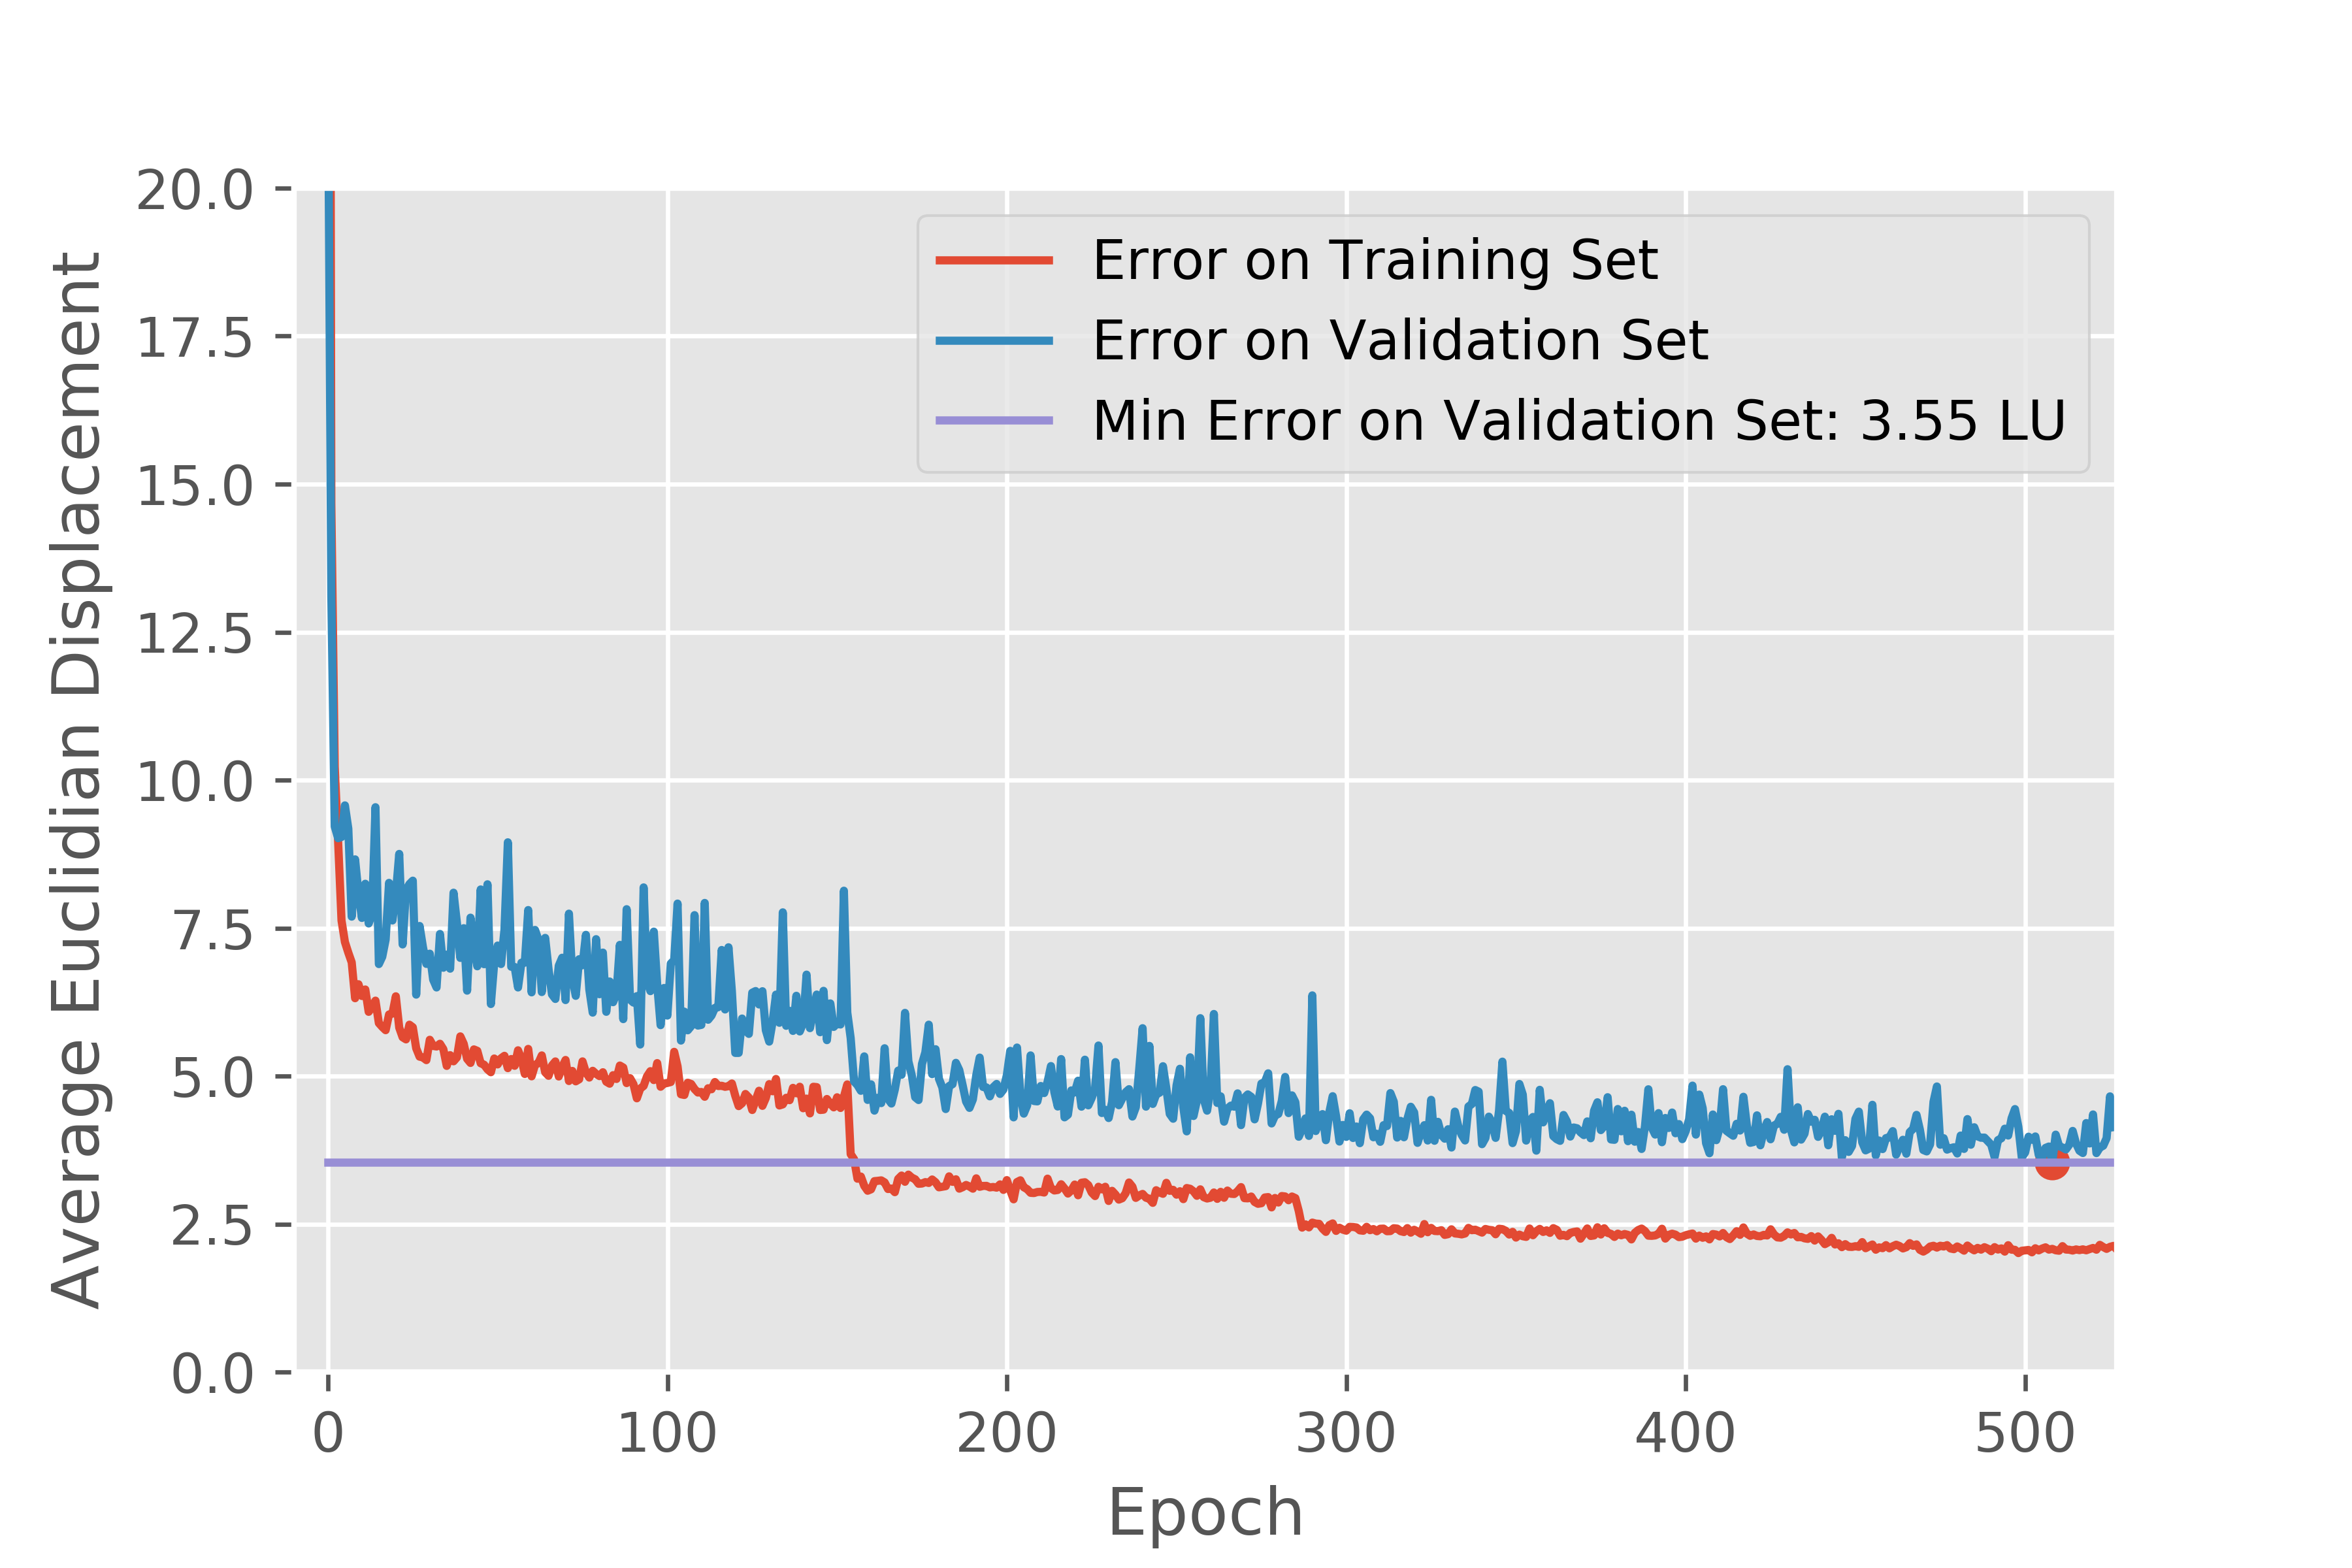
\includegraphics[width=0.99\textwidth]{figures/reg_plot1.pdf}
	\caption{Development of the average euclidean displacement by epoch on the training- and validation set.}
	\fontsize{3}{2}
	\label{fig:autoencoder_architecture}
\end{figure}

\subsubsection{Limitations of the Model}
This experiment is an attempt to show the principle ability to use convolutional neural network to solve a task with a time-series as input. This special posed task of the inverse problem of ECG gave comparably good results. This shows that the neural network is able to process through a temporally random selected section of fixed length, which makes it clear that it recognizes a pattern in the signals regardless of the phase of the concentric wave.
The simulated heart contains of around 10000 elements on the surface, which can represent an approximate source of the concentric wave. While having 1024 simulation, having unique starting conditions, around 10\% of the available sources are already covered. 
The properties of a simulation differ only in the location of the pacing events that cause the concentric wave. It is possible that some training and test simulations differ very little from each other, if the locations of the pacing events are very close to each other. In this case it may not be possible to speak of a truly unknown data set. The average minimal distance from a test-simulation to the next training-simulation is around 2.47 LU. It shows that the neural network is trained with pacing positions, which are not far distant from the test-simulations. Furthermore, the neural networks average displacement of the predictions on the test-dataset is bigger than the average distance to the next training simulation.
Nevertheless, the same CNN is able to handle a dataset with additional Gaussian noise. The training on the same dataset with this noise with $\sigma=0.05$ got displacements as shown in table \ref{tab:noise}:

\begin{table}[h]
    \centering
    \begin{tabular}{|c|c|}
    \hline
    training set & test set\\
    \hline
    1.69 & 3.15 \\
    \hline
    \end{tabular}
    \caption{Average displacement of the prediction from the CNN on the training- and test-dataset, additional Gaussian noise with $\sigma=0.05$ is added to the normalized data (this means that a 5\% error is included).}
    \label{tab:noise}
\end{table}

The average displacement on the test-dataset did not increase much (a difference of 0.04LU).
% Next:
    % more noise, geometrical noise
    % more complex simulations
    %


    \chapter{Under-surface prediction}
%The following experiment now considers a surface to predict the dynamic at hidden layer under the surface.
%The goal of the experiment is to have an idea about the limitations on this specific task. The following aspects are relevant in the research:
%\begin{itemize}
%    \item How does the length of the input affect the quality of the results in dependency of the depth.
%    \item Is it an advantage to consider the dynamic at the surface in the future to predict a hidden layer.
%    \item How much does random behaviour affect the quality of the prediction.
%    \item Does spatial correlation between two layer, correlate with the quality of the prediction.
%\end{itemize}

%Each of these questions aim to build a guideline for future work on a heart simulation, which obviously has a much more complicate structure. This experiment under thinkable simple conditions has the function as a playground to test which parameter are critical, and which configuration has the best compromise.

% What, in broad terms
This chapter is about the second numerical experiment. The basis for it is a 3D-simulation of the time evolution of an excitable medium. The question is to what extent a machine learning model respectively a neural network can predict a system quantity inside of the 3D structure which is not \textit{visible} from outside. The input to the neural network and its prediction are values of the same system quantity, where the input is recorded on the surface of the 3D structure over a period of time. Here, \textit{not visible} means that the neural network has no explicit information about the data inside the 3D structure that it is supposed to predict. Only on the basis of the surface it is to extrapolate these. The posing of this problem is motivated by a possible transfer to heart dynamics. It would be a matter of inferring the inner dynamics from the surface dynamics which results from the electrical activity of the heart muscle cells. 

In general, one wants to get as much information from the heart's activity as possible with minimally invasive or non-invasive measurement methods to make an intervention to obtain this information as low-risk and cost-effective as possible. While the first experiment was about drawing conclusions about the electrical activity at the surface of the heart from the ECG signals, one prospect of this experiment is to predict the interior electrical activity, based on the heart's surface.

% Storyline
%While the previous experiment was about information gain of the surface of the heart, based on an ECG-signal, this experiment now takes into account the surface to get information about the system under the surface.

% Previous work
Some experiments have been done by [xx] or [yy]. While these approaches are based on real data and , in this work I will go a step back and want to study the limits of machine learning models that faces up to the task mentioned above, while having \textit{perfect} surface information. \textit{Perfect} means here, unlike in real experiments, that the data does not have any noise\footnote{If we ignore the numerical error.}. Furthermore, with choosing a cube as comparatively simple geometry, I regard this as a base study about the limitations of machine learning models in this kind of problem. This numerical experiments tests two different sequence-to-sequence LSTM architectures on two different parameter sets within the model for excitable media where one builds \textit{concentric waves} and the other \textit{breaking spiral waves}, as visualized in figure [xx]. Details concerning the characteristics of these regimes are explained in section [yy]

How a possible transfer of this experiment to biological data can be realized and to what extent it would build on the results of this study is discussed in chapter xx.

% Exact input and output

% Excitable media model and hyperparamter
% Barkley, and two regimes, 

% Machine learning models
% LSTM and STLSTM

% Leserorientierung

% Simulation, (chaos, concentrisch)
% Training of neural network in general,
% Optimal parameter search (also with respect to graphics card, see appendix)
% Study: Varying time-span from input. The more time steps the better? (-->till certain point not better)
% Comparison between LSTM and STLSTM

% Zu erklären: Two regimes, 

\section{Methods}\label{cap:diver_methods}
Goal is to train a machine-learning model which takes into account the time evolution of the $u$-value of the Barkley model \cite{Barkley_2008} at the surface, to predict at a certain time point the $u$-value under the surface. In this chapter I introduce the process of generating training- and validation data and elaborate some characteristics of the simulations.

\subsection{Model}
There are various models to describe the heart dynamic but since this experiments goal is to reconstruct hidden regions under the surface qualitatively, the model does not have to describe the heart dynamic as accurate as possible. In this work the Barkley model is used, which is a system of two coupled differential equations which build a reaction-diffusion system. It is a comparably\footnote{Compared for example with the Hodgkin-Huxley model which consists of three coupled differential equations.} simple model and consists of two variables $u$ and $v$ which are dependent on the equations

\begin{align}
    \frac{\partial u}{\partial t}&=D\cdot \nabla^2u+\frac{1}{\varepsilon}(1-u)\left(u-\frac{v+b}{a}\right)\notag\\
    \frac{\partial v}{\partial t}&=u^{\alpha}-v.\notag\\
\end{align}

The parameter $\epsilon$ controls . A bigger value for $a$ increased the excitation duration while an increasing fraction between $b$ and $a$, $\frac{b}{a}$, results to a larger excitability threshold. In this work the value for $\alpha$ is set to 1. The exact values for both regimes are in table (\ref{tab:simulation_parameter}).

\subsubsection{Simulation}
The Barkley-model will be simulated in three dimensions in which the discretised diffusion operator $\nabla^2$ is here described through a 7-point stencil such that

\begin{align}
    \left(\nabla_7^2u\right)_{i,j,k}=\frac{u_{i-1,j,k}+u_{i+1,j,k}+u_{i,j-1,k}+u_{i,j+1,k}+u_{i,j,k-1}+u_{i,j,k+1}-6u_{i,j,k}}{\Delta s^2},
\end{align}

where the indices $i$,$j$ and $k$ stand for the discretised position within the $x$-$y$-$z$-cube and $\Delta s$ the spatial discretisation. A simulation step in time will be calculated through the explicit Euler method with

\begin{align}
    u(t+1)&=u(t)+\Delta t\frac{\partial u(t)}{\partial t}\notag\\
    v(t+1)&=v(t)+\Delta t\frac{\partial v(t)}{\partial t}.\notag\\
\end{align}

that a time-step within the Barkley model is described as 

\begin{align}
    u(t+1)_{i,j,k}&=u(t)_{i,j,k}+\Delta t\cdot\left(D\cdot \left(\nabla_7^2u\right)_{i,j,k}+\frac{1}{\varepsilon}(1-u(t)_{i,j,k})\left(u(t)_{i,j,k}-\frac{v(t)_{i,j,k}+b}{a}\right)\right)\notag\\
    v(t+1)_{i,j,k}&=v(t)_{i,j,k}+\Delta t\cdot\left(u(t)_{i,j,k}^{3}-v(t)_{i,j,k}\right)\notag\\
\end{align}

The hyperparameter $a$, $b$, $\varepsilon$, $\Delta t$ and $\Delta s$ are arbitrary chosen for two regimes, in which one builds concentric waves and the other shows a chaotic behaviour. The exact values are shown in table (\ref{tab:simulation_parameter}). The simulation is implemented in python with orientating on the code for a 2D Barkley simulation by Roland Zimmermann \cite{zimmermann}.
%\subsection{Data-assimilation}
\subsubsection{Hyperparameter and simulation size}

\begin{table}[h]
    \centering
    \begin{tabular}{|c|c|c|}
    \hline
    & Non-chaotic & chaotic\\
    \hline
    $a$ & 0.6 & 1.0 \\
    \hline
    $b$ & 0.01 & 0.15 \\
    \hline
    $\epsilon$ & 0.02 & 0.02 \\
    \hline
    $\Delta t$ & 0.01 & 0.01 \\
    \hline
    $\Delta s$ & 0.1 & 0.1 \\
    \hline
    $\alpha$ & 1 & 1\\
    \hline
    \end{tabular}
    \caption{Barkley simulation configurations.}
    \label{tab:simulation_parameter}
\end{table}

The parameter set for 'non-chaotic' is adjusted to build concentric waves (as visualized in figure xx), while the chaotic regime produces breaking spiral waves. The parameter adjustment for $a$ and $b$ is based on a paper by Alonso et al. \cite{alonso_taming_2003} in which they study the parameter-space of the Barkley model and their influence within a 3D-simulation.

These two parameter regimes 
The parameter are specifically chosen to generate
Both simulations are embedded on the cube with 120 unit in each dimension. 

\subsubsection{Characteristic units}

To have a more intuitive understanding about time- and spatial sized which are taken into account by the models I apply characteristic dimensions as following:

\begin{itemize}
    \item Length $L_c$: The characteristic length $L_c$ is defined by average thickness along the normal of a wave front. Here it is estimated manually by taking the average from 32 measurements $\iota=\overline{(\iota_1,...,\iota_{32})}$. The length follows to $L_c=\iota\cdot\Delta\text{s}$.
    \item Velocity $V_c$: The velocity is measured by counting the amount of discrete length units $\Delta s$ which are passed per discrete time step $\Delta t$. To minimize the error, the distance is measured after 64 time-steps, and the average of 32 of these measurements build the characteristic velocity as $V_c=\nu\cdot\Delta\text{s}/\Delta\text{t}$.
    
    \item Time $T_c$: The characteristic time is applied by the time a wave needs to travel the characteristic length. It follows the time according to $T_c=L_c/V_c\equiv\iota/\nu\cdot\Delta\text{t}=:\tau\cdot\Delta\text{t}$.
    %Why the connection of the length and time is motivated by the problem definition is explained in chapter (231).
\end{itemize}

The resulting values for $\iota$, $\nu$ and $\tau$ are shown in table (\ref{tab:characteristic}). 

\begin{table}[h]
    \centering
    \begin{tabular}{|c|c|c|}
    \hline
    & 1: Non-chaotic & 2: chaotic\\
    \hline
    $\iota$ & 10.50$\pm$1.45 & 3.15 \\
    \hline
    $\nu$ & 0.155$\pm$0.041 & 3.15 \\
    \hline
    $\tau$ & 67.74$\pm$20.24 & 3.15 \\ % 67.74
    \hline
    $L_c$ & 1.05$\pm$0.15 & 3.15 \\ % 67.74
    \hline
    $V_c$ & 1.55$\pm$0.41 & 3.15 \\ % 67.74
    \hline
    $T_c$ & 0.68$\pm$0.20 & 3.15 \\ % 67.74
    \hline
    \end{tabular}
    \caption{Characteristic dimensionless units for the two Barkley configurations.}
    \label{tab:characteristic}
\end{table}

Intuitively, a wave-front which propagates along the normal of the surface in a depth of $\iota\cdot\text{ds}$, needs in average $\tau$ discrete time steps to be recognisable at the surface. %The time a structure needs to be visible in future time step at surface is a considered quantity in the experiment. %In chapter (RESULTS) I will show that if the model takes into account future time steps, it is able to reconstruct non-surface structures at a given time point in the past.

\subsection{Generating data and preprocessing}
% Simulation output --> what to do for model
% float64 to int8
% - reshape to single datapoints, save as pytorch-dataset
%120x120x120 --> (X,y) == (B,T,D,H,W), 
%\section{Seq2Seq neural network for under-surface prediction}

The following described procedure of data generation and preprocessing is the same for both regimes. The only difference is the adjusting of hyperparameters according to table (\ref{tab:simulation_parameter}).

\subsubsection{Data generation}
As mentioned before, I consider in the experiment the $u$ value of the Barkley model. Since the cube has an expansion of 120 discretised units in each spatial dimension, a snapshot of the $u$ value is a tensor of order 3 with a dimensionality of (120,120,120)=(depth, height, width). 
In a single simulation each snapshot is recorded after 16 discrete time-steps from the previous snapshot over a span of 512 steps. Therefore, each simulation saves a tensor with the dimensionality of (32,120,120,120). The recording starts after an initial phase of 2048 time steps. Basis for the preprocessing step, which I explain in the following, are 256 of these simulations for each regime (concentric and chaotic). Here I use $X$ to describe the data the machine learning model gets as input to predict $y$.


\subsubsection{Preprocessing}
% X and y describing
Since a cube has 6 sides, here each simulation produces 6 time-series from the surface. The corresponding $y$-data is a tensor which saves the $u$-value for the next lower layers below the respective surface. The maximal depth is set at 32 discrete spatial units. Therefore, from 256 single simulations, one gets $256\cdot6=1536$ X-y-pairs with $X\in R^{32\times1\times120\times120}$ and $y\in R^{1\times32\times120\times120}$. It is divided into a training-set (1024 pairs) and validation set (512 pairs). Note that the dimensions stand for (time-steps$\times$depth$\times$height$\times$width). The $X$-data includes only the surface of the cube, therefore the depth is always 1, while $y$ is the prediction at a certain time-step till a maximal depth of 32.
The data within the simulations are computed as float64 (means each single value needs 64 bit of storage with the float data type). Nonetheless it is possible without a great loss on information to convert the data into one-byte-integers (int8) to save storage. Therefore, $X$ and $y$ are rescaled into the range of int8 (-127 to 128). 

Within the training process, the data again has to be rescaled into the range from 0 to 1. This is done with the help of a pytorch dataloader, whose functionality is explained in \ref{cap:pytorch}.

\subsection{C-LSTM and ST-LSTM}
In section (\ref{cap:seq2seq}) a general design of sequence-to-sequence models with recurrent neural networks was introduced. In this section, I present the exact composition of the models used in this experiment. The two models differ only in the implementation of their recurrent cells, which are the C-LSTM cell (see section \ref{cap:CLSTM}) and the ST-LSTM cell (see section \ref{cap:STLSTM}).

The models are based on the same architecture as visualized in figure (\ref{fig:seq2seq}). The encoder- (embedding) and decoder-networks (colored green in figure (\ref{fig:seq2seq})) are time distributed, which means that the same network is used separately for each time point of an input sequence. Encoder and decoder are convolutional neural networks whose architecture is visualized in figure (\ref{fig:encoder}) and (\ref{fig:decoder}). Some convolutional layers have a stride-parameter of 2, which reduces the spatial dimensionality by the factor of two. Therefore, with an input $X$ with $X\in R^{\text{batch}\times\text{time-steps}\times\text{depth}\times\text{height}\times\text{width}}$, the encoder reduces it to $X_{\text{out}}\in R^{\text{batch}\times\text{time-steps}\times\text{features}\times\text{height/2}\times\text{width/2}}$. Note, that instead of \textit{depth}, the third dimension represents now the number of channels, which is a hyperparameter of a convolutional layer as introduced in section (\ref{cap:multichannel}). The value is always set for all convolutional layers within the encoder and decoder to 64.

\begin{figure}[!tbp]
  \centering
  \begin{minipage}[b]{0.4\textwidth}
    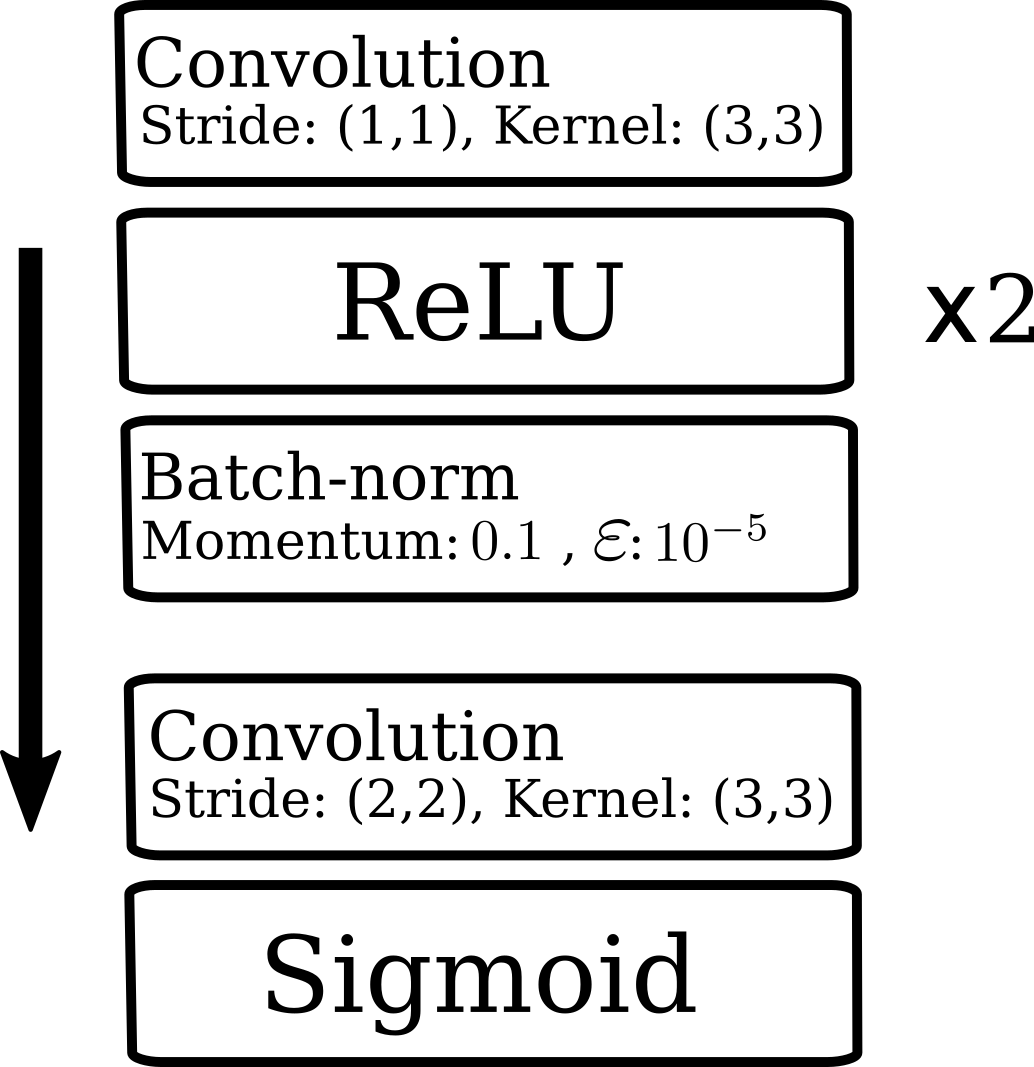
\includegraphics[width=\textwidth]{figures/encoder.png}
    \caption{Encoder}
    \label{fig:encoder}
  \end{minipage}
  \hfill
  \begin{minipage}[b]{0.4\textwidth}
    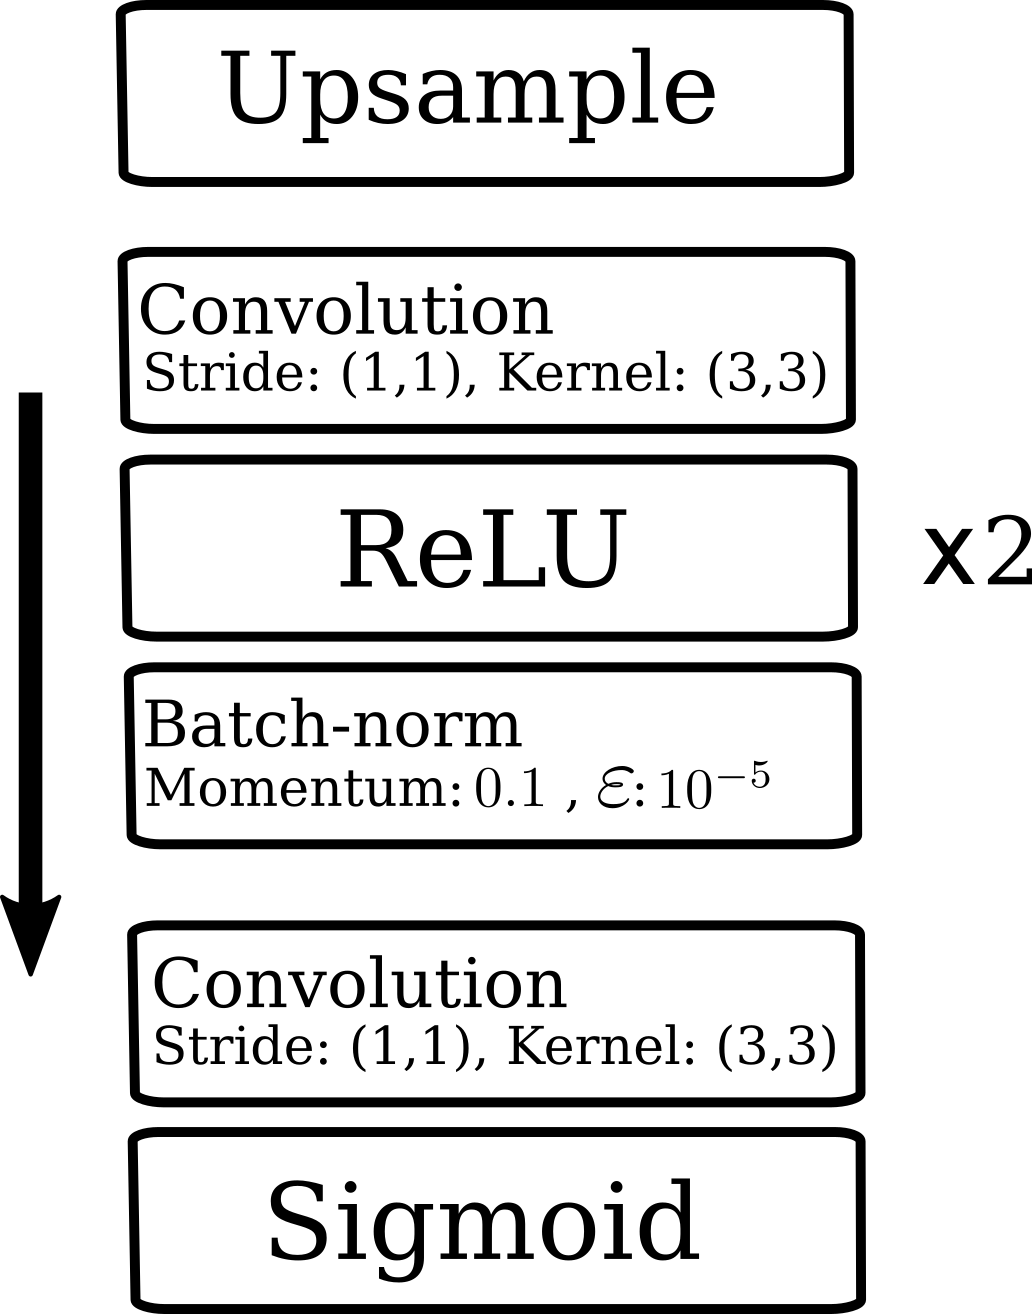
\includegraphics[width=\textwidth]{figures/decoder.png}
    \caption{Decoder}
    \label{fig:decoder}
  \end{minipage}
\end{figure}

\subsection{Optimal hyperparameter search}
While the architecture of the two approaches (C-LSTM and ST-LSTM) will be considered as given, I search for the optimal hyperparameter for the training process. These are the loss-function, learning rate, batch size and the optimizer. Table (\ref{tab:gridsearch}) shows the values of the hyperparameters that are varied, as well as the ideal parameter combination.

\begin{figure}[ht]
    \center
    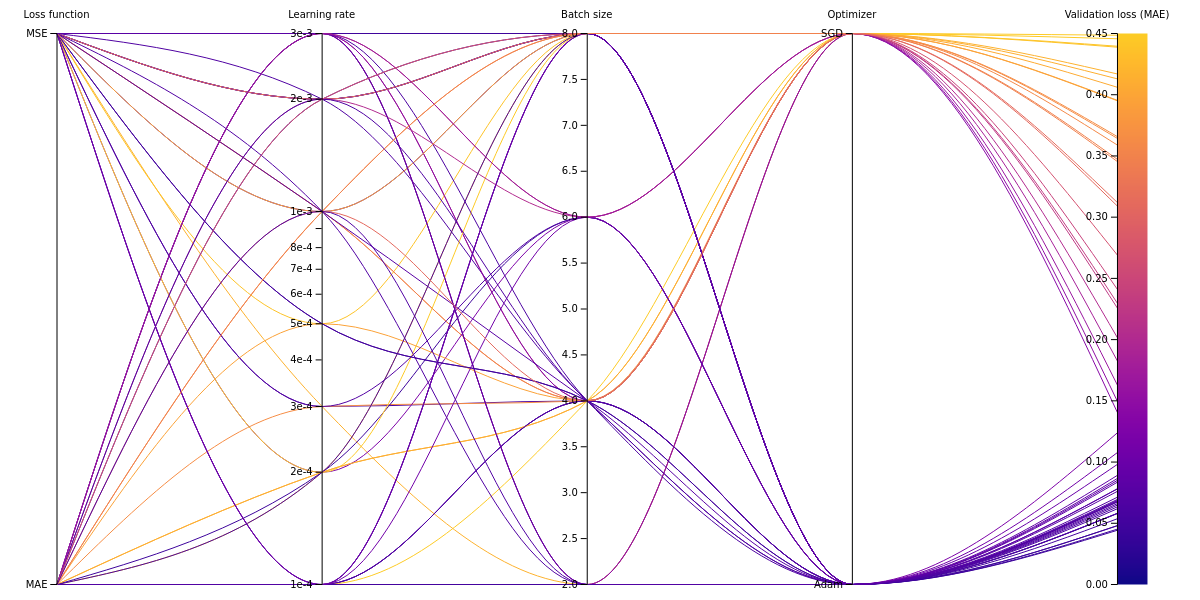
\includegraphics[width=0.99\textwidth]{figures/sweep_clstm.png}
	\caption{Results of a grid-search with 4 varying hyperparameter. The hyperparameter in this graphic are sorted by its influence to the loss from less important (left) to more important (right) (the importance is sorted by random forest feature importance to calculate how much a hyperparameter choice played a role in the result according to the metric). The parameter-variations and best combination are in table (\ref{tab:gridsearch}). The loss is calculated after one epoch with 1024 examples.}
	\label{fig:sweep_clstm}
\end{figure}

\begin{table}[h]
    \centering
    \begin{tabular}{|c|c|c|}
    \hline
    Parameter & Values & Best value\\
    \hline
    \hline
    Loss function & MSE, MAE & MSE\\
    \hline
    Learning rate & $\{1,2,3,5\}\cdot10^{-4}$, $\{1,2,3\}\cdot10^{-3}$ & $10^{-4}$\\
    \hline
    Batch-size & 2,4,6,8 & 4\\
    \hline
    Optimizer & SGD\footnote{Stochastic gradient descent}, Adam & Adam \\ % 67.74
    \hline
    \end{tabular}
    \caption{Characteristic dimensionless units for the two Barkley configurations.}
    \label{tab:gridsearch}
\end{table}

\section{Specific studies}
% Including varying time-steps, comparison.
% Qualitative results, can structures be detected?
% Performance on chaos regime, plus using ST-LSTM
In this work I consider four studies. Included are the two described models C-LSTM and ST-LSTM to perform tasks within two regimes. All studies have in common, that a machine learning model takes as input a temporal sequence of the $u$-value from the Barkley model, which is one side of the surface of the 3D simulation with the shape of a cube.

\subsection{Influence of the input-sequence length}
First, I vary the length of the temporal sequence as input. Goal of this study is to find in 

\subsection{Qualitative detection of hidden structures}
In the second study I figure out if hidden structures can be deteced by 
\subsection{Comparison C-LSTM, ST-LSTM}
\subsection{Performance of chaotic regime}

First, I vary the length of the time interval that the models use as a basis for their prediction. In excitable media, an excitation has an increasing global influence with time passed. This leads to the assumption that excitations below the surface have an influence on the surface dynamics after a certain time passed. The first study is about the question if or rather in which amount this influence can affect the prediction accuracy. The characteristic velocity, which I introduced in chapter 4, plays an important role in this process. Since in both regimes (see table xx) build wave-fronts, the average speed of these wave fronts is used as characteristic velocity. 

\section{Results and validation}
Influence of the input-sequence length

The results are separated into three parts. Firstly I show the general ability of detecting hidden structures with a surface-sequence. These results are based on experiments which are performed only with the C-LSTM in regime 1 (see table (\ref{tab:simulation_parameter}) at \textit{non-chaotic} for the exact Barkley-hyperparameter).

The in the second part, I compare the results of C-LSTMs and ST-LSTMs
% Plot example: Time-steps sättigung, depth of 5, + depth of 

The plot show curvature which are smoothed with the Savitzy-Golay filter \cite{Savitzky1964SmoothingAD} to increase the visibility of the curves. Without the filter they would be very noisy.

%\begin{figure}[ht]
%    \center
%    \includegraphics[width=0.99\textwidth]{figures/cubeplots1.png}
%	\caption{Hyperparameter search, sorted by importance. The validation loss is calculated after one epoch with 1024 examples. The model considers in the output a depth of 8 with having an input sequence of length 8.}
%	\label{fig:sweep_clstm}
%\end{figure}

\begin{figure}[!htb]
    \center
    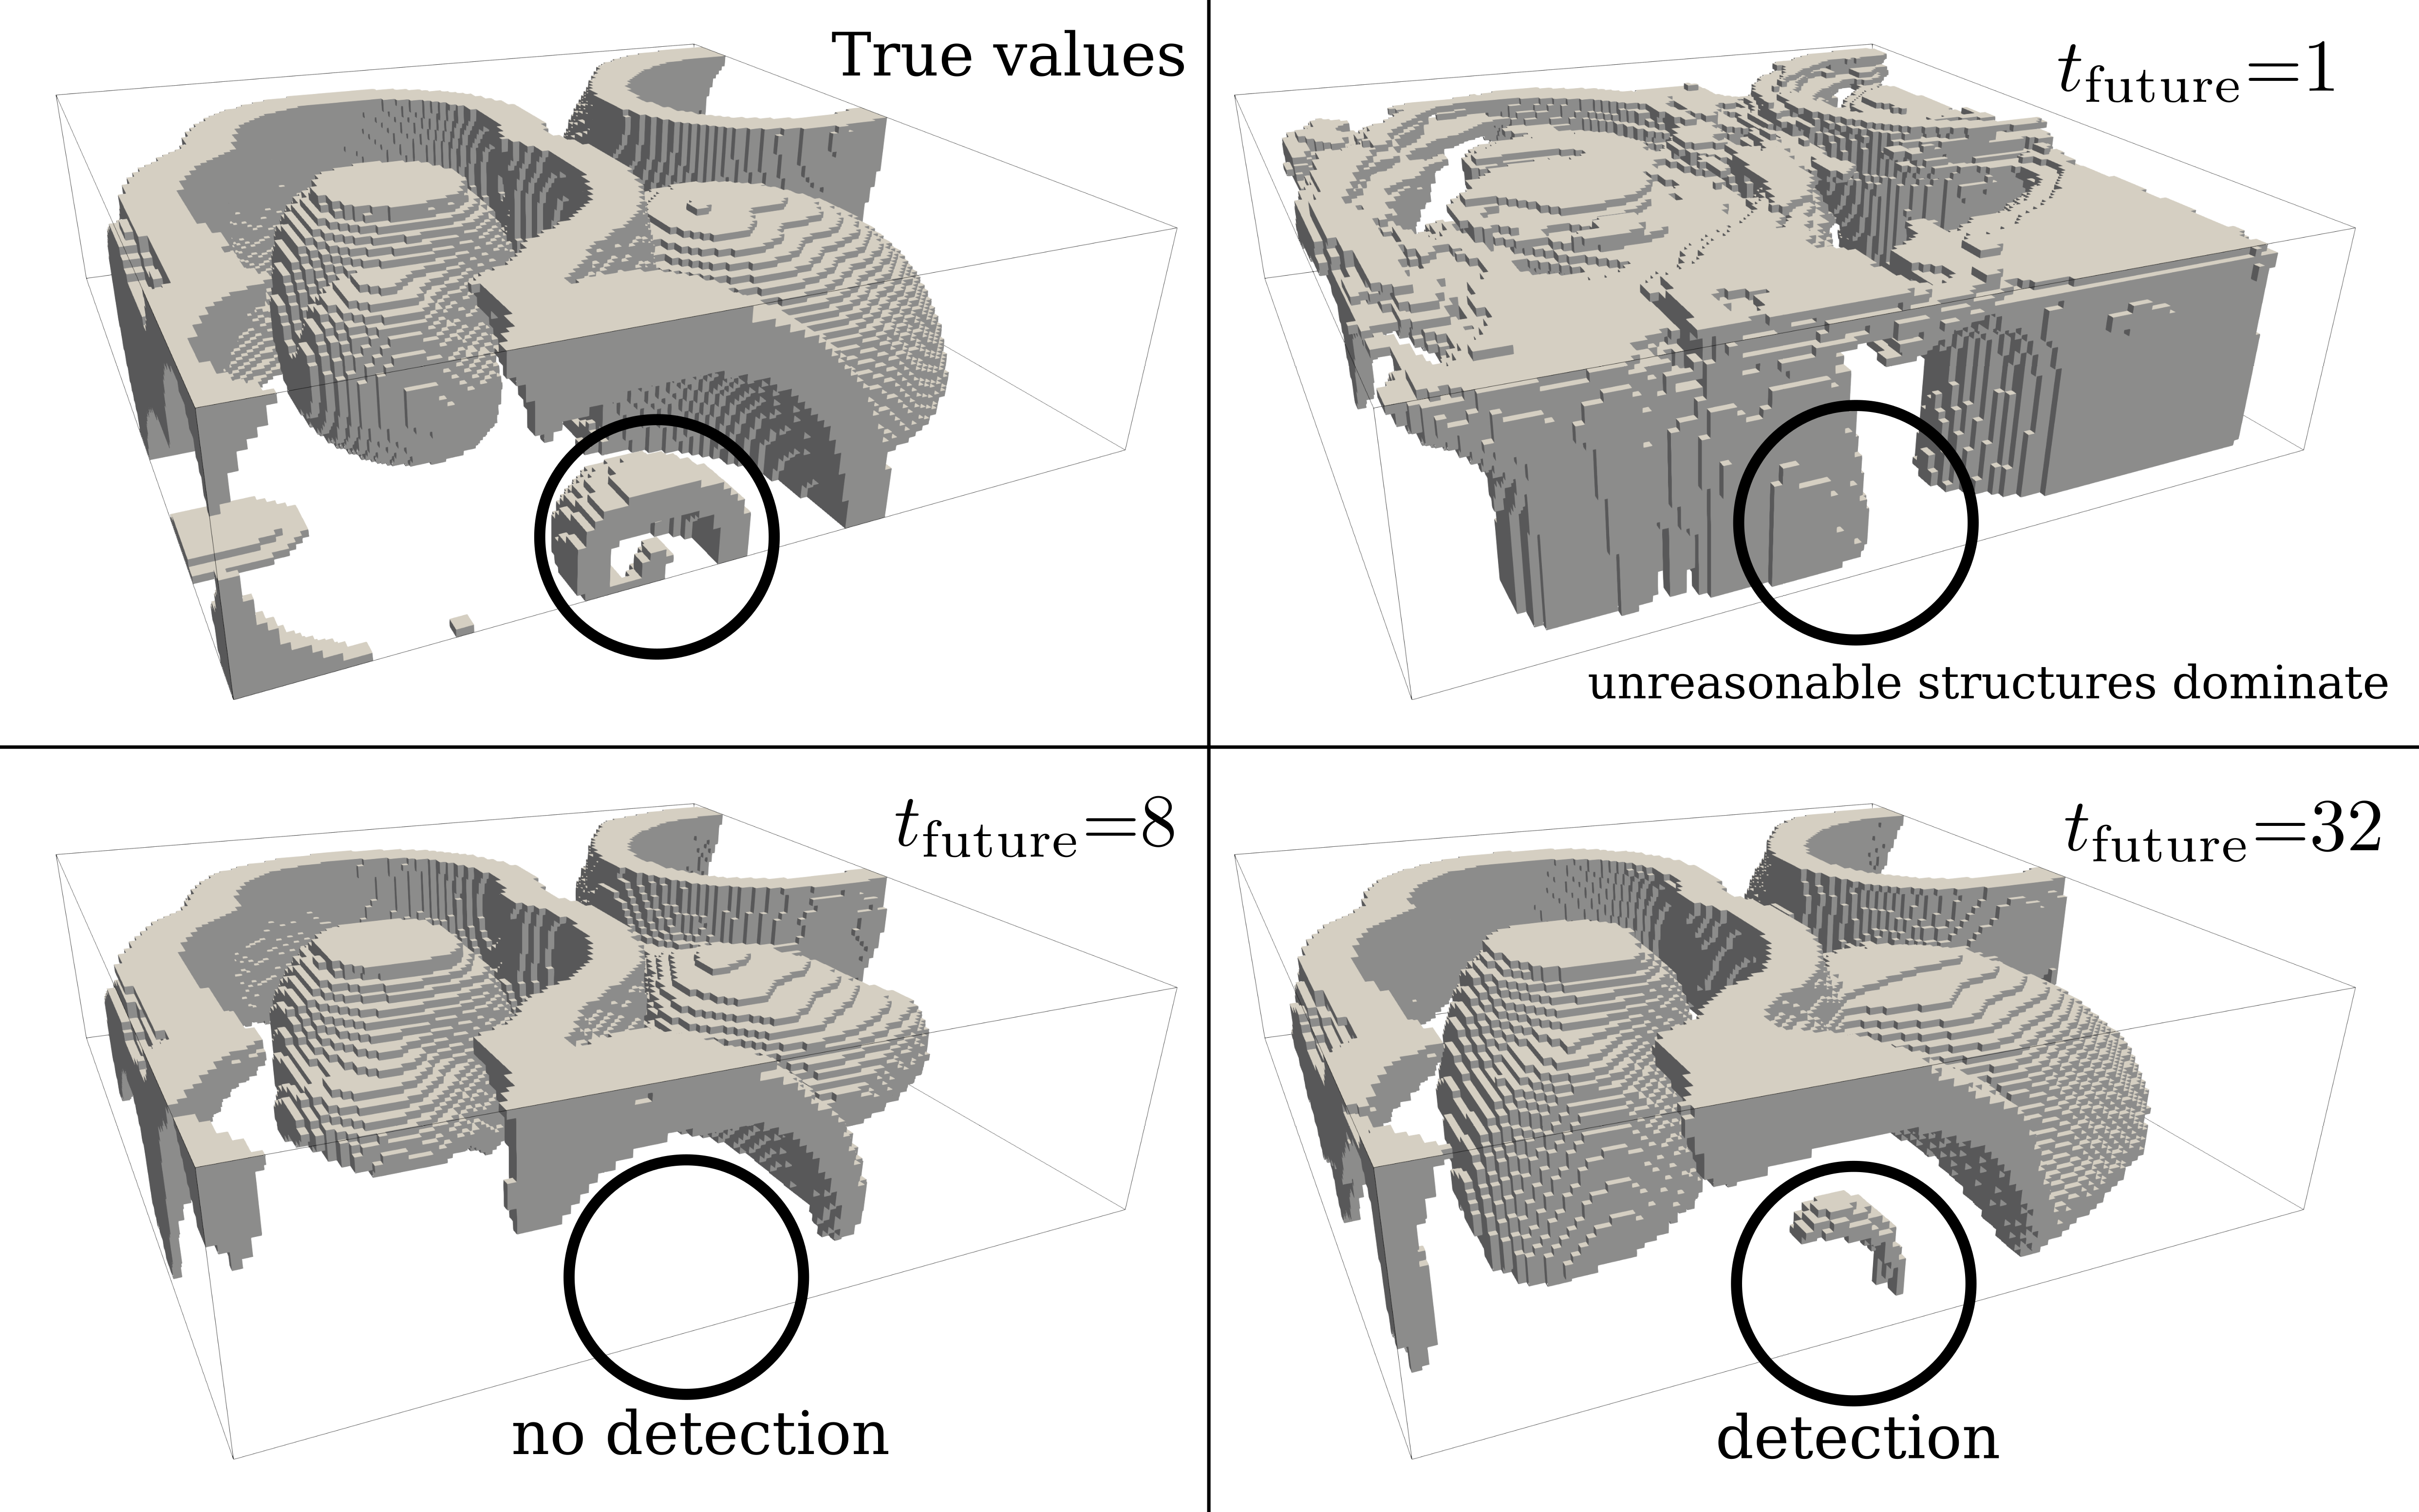
\includegraphics[width=0.95\textwidth]{figures/CLSTM_p361_d32_t_1_8_32.png}
	\caption{Comparison, a point is visualized as long its value is over 0.5.Comparison, a point is visualized as long its value is over 0.5.Comparison, a point is visualized as long its value is over 0.5.}
	\label{fig:clstm_3d_p361}
\end{figure}

\begin{figure}[!htb]
    \center
    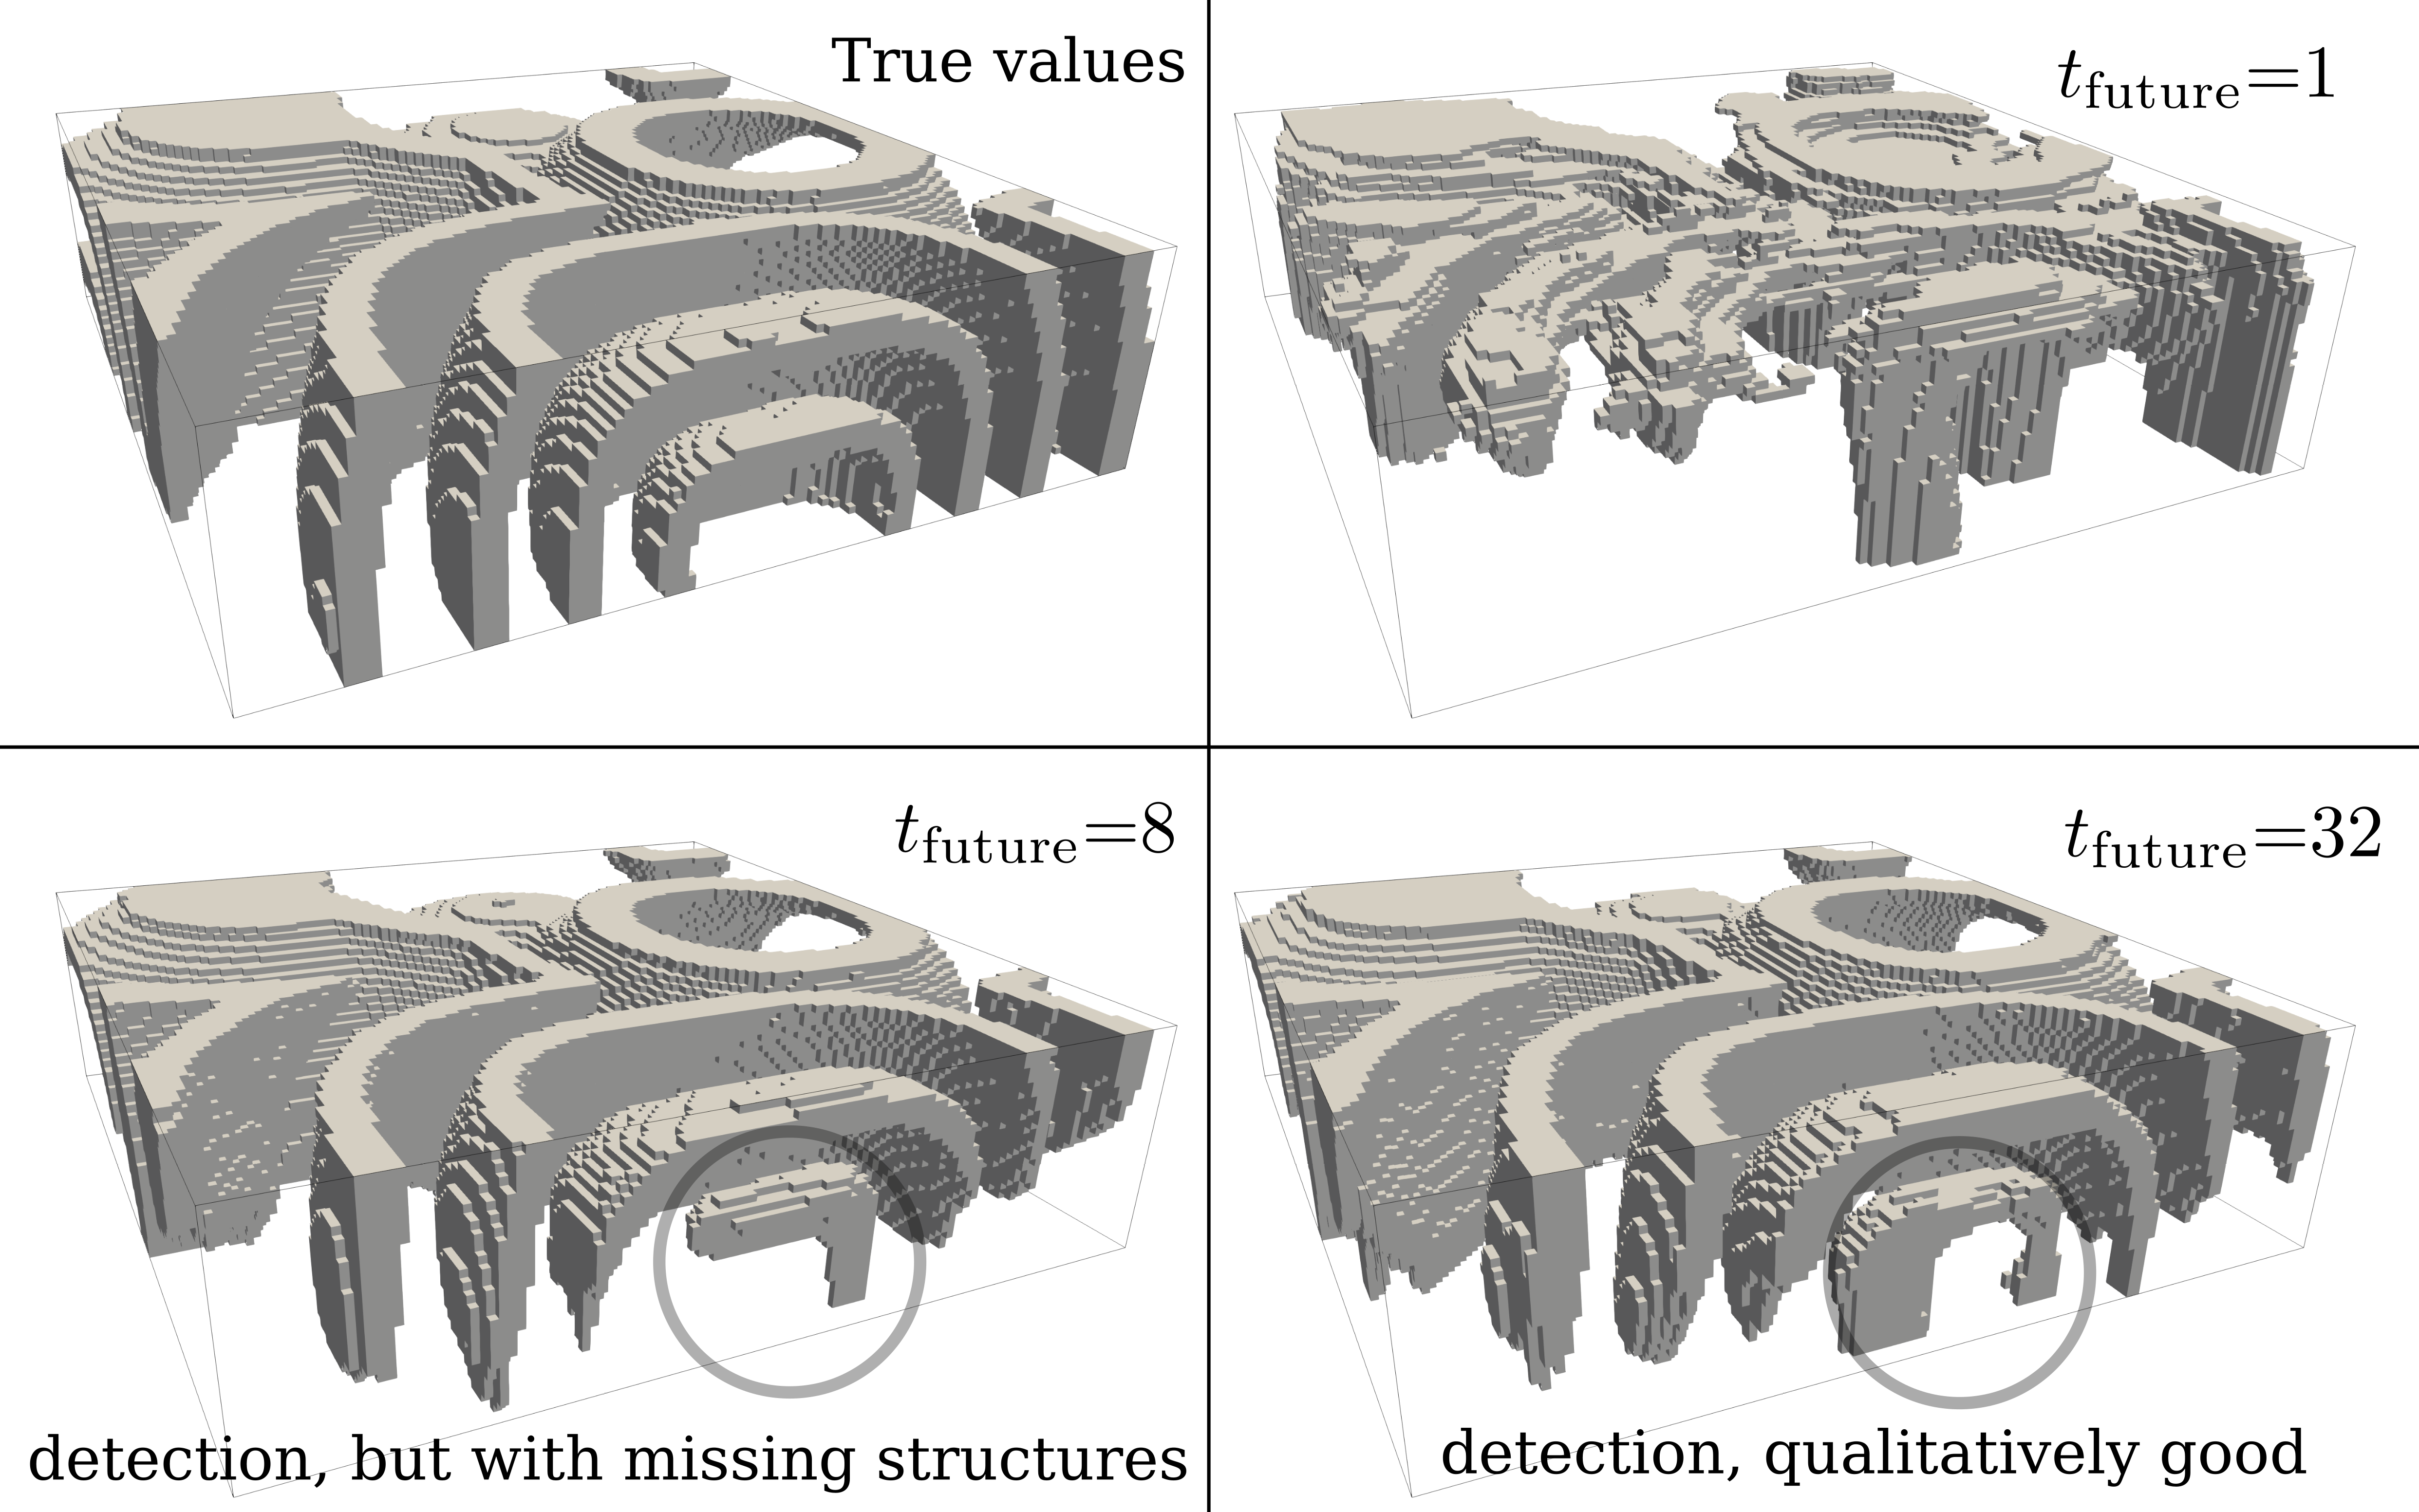
\includegraphics[width=0.95\textwidth]{figures/CLSTM_p26_d32_t_1_8_32.png}
	\caption{Comparison, a point is visualized as long its value is over 0.5.}
	\label{fig:clstm_3d_p26}
\end{figure}

%\section{Discussion}
%\subsection{iECG}
%\subsection{Under-surface predictor}
\textbf{What are the results}
What is the research usable for:
    - A study how good models work in this kind of problem, if it is even possible to detect hidden structures. And the work shows, it definitely is able to detect some of these structures under good circumstances and not in real time because it needs data from the future. Nonetheless some patterns can periodically. 

In a periodic dynamic, is it enough to have the surface-data? 
What is the core of the problem in terms of machine learning?
What is proven?
How can the results be useful for future work?
    - Can the models respectively the problem formulation be generalized, for example for a more complex geometry with the topological description of a doughnut.
How can approaches be embedded in the big field of machine learning 
    - shows one approach with is proven in a number of different fields to be able to build a state-of-the-art model or was state-of-the-art in a certain time.
    



    \chapter{Outlook}
Outlook and so
    \chapter{Summary}
    
    %\chapter{Outlook}
Outlook and so
    %\input{content/appendix}
    
    %\bibliographystyle{agsm}
    \bibliographystyle{unsrt}
    \begin{flushleft}
        \bibliography{references}
    \end{flushleft}
    \Declaration
\end{document}
